% Preambel mit Einstellungen importieren
% Document type and used packages
\documentclass[open=right, % Kapitel darf nur auf rechten Seite beginnen
    paper=A4,               % DIN-A4-Papier
    a4paper,                % DIN-A4-Papier
    12pt,                   % Schriftgöße
    headings=small,         % Kleine Überschriften
    headsepline=true,       % Trennlinie am Kopf der Seite
    footsepline=false,      % Keine Trennlinie am Fuß der Seite
    bibliography=totoc,     % Literaturverzeichnis in das Inhaltsverzeichnis aufnehmen
    twoside=on,             % Doppelseitiger Druck - auf off stellen für einseitig
    DIV=7,                  % Verhältnis der Ränder zum bedruckten Bereich
    chapterprefix=true,     % Kapitel x vor dem Kapitelnamen
    cleardoublepage=plain]{scrbook}

% Pakete einbinden, die benötigt werden
\usepackage{pdflscape}
\usepackage{scrpage2}
\usepackage[utf8]{inputenc}       % Dateien in UTF-8 benutzen
\usepackage[T1]{fontenc}          % Zeichenkodierung
\usepackage{graphicx}             % Bilder einbinden
\usepackage[main=ngerman, english]{babel}       % Deutsch und Englisch unterstützen
\usepackage{xcolor}               % Color support
\usepackage{amsmath}              % Matheamtische Formeln
\usepackage{amsfonts}             % Mathematische Zeichensätze
\usepackage{amssymb}              % Mathematische Symbole
\usepackage{float}                % Fließende Objekte (Tabellen, Grafiken etc.)
\usepackage{booktabs}             % Korrekter Tabellensatz
\usepackage{wrapfig,lipsum}		  % mit Text umflossene Tabellen
\usepackage[printonlyused]{acronym}  % Abkürzungsverzeichnis [nur verwendete Abkürzugen]
\usepackage{makeidx}              % Sachregister
\usepackage{listings}             % Source Code listings
\usepackage{listingsutf8}         % Listings in UTF8
\usepackage[hang,font={sf,footnotesize},labelfont={footnotesize,bf}]{caption} % Beschriftungen
\usepackage[scaled]{helvet}       % Schrift Helvetia laden
\usepackage[absolute]{textpos}	  % Absolute Textpositionen (für Deckblatt)
\usepackage{textcomp}			  % Für °-Symbol
\usepackage{gensymb}			  % Für °-Symbol
\usepackage{calc}                 % Berechnung von Positionen
\usepackage{blindtext}            % Blindtexte
\usepackage[bottom=40mm,left=35mm,right=35mm,top=30mm]{geometry} % Ränder ändern
\usepackage{setspace}             % Abstände korrigieren
\usepackage{ifthen}               % Logische Bedingungen mit ifthenelse
\usepackage{scrhack}              % Get rid of tocbasic warnings
\usepackage[pagebackref=false,german]{hyperref}  % Hyperlinks
\usepackage[all]{hypcap}          % Korrekte Verlinkung von Floats
\usepackage[autostyle=true,german=quotes]{csquotes}   % Zitate
\usepackage[backend=bibtex,
isbn=false,                     % ISBN nicht anzeigen, gleiches geht mit nahezu allen anderen Feldern
sortlocale=de_DE,               % Sortierung der Einträge für Deutsch
%sortlocale=en_US,              % Sortierung der Einträge für Englisch
autocite=inline,                % regelt Aussehen für \autocite (inline=\parancite)
hyperref=true,                  % Hyperlinks für Ziate
style=nature,				  		% Zitationsstil in Overleaf verfügbar
%style=numeric,                 % Zitate als Zahlen [1]
%style=alphabetic               % Zitate als Kürzel und Jahr [Ein05]
%style=authoryear               % Zitate Author und Jahr [Einstein (1905)]
]{biblatex}                     % Literaturverwaltung mit BibLaTeX
\usepackage{rotating}           % Seiten drehen
\usepackage{tabularx}			% Automatischer Zeilenumbruch in Tabellen mit \begin{tabularx} ... \end{tabularx}
\usepackage{array,multirow,graphicx} % Reihenweise zusammgnefügte Tabellenelemente und vertikale Textausrichtung 
% Farben für Codeexamples
\definecolor{mygreen}{RGB}{28,172,0} % color values Red, Green, Blue
\definecolor{mylilas}{RGB}{170,55,241}



%\usepackage{harveyballs}          % Harveyballs

\setlength{\bibitemsep}{1em}     % Abstand zwischen den Literaturangaben
\setlength{\bibhang}{2em}        % Einzug nach jeweils erster Zeile

% Trennung von URLs im Literaturverzeichnis (große Werte [> 10000] verhindern die Trennung)
\defcounter{biburlnumpenalty}{10} % Strafe für Trennung in URL nach Zahl
\defcounter{biburlucpenalty}{500}  % Strafe für Trennung in URL nach Großbuchstaben
\defcounter{biburllcpenalty}{500}  % Strafe für Trennung in URL nach Kleinbuchstaben

% Farben definieren
\definecolor{linkblue}{RGB}{0, 0, 100}
\definecolor{linkblack}{RGB}{0, 0, 0}
\definecolor{comment}{RGB}{63, 127, 95}
\definecolor{darkgreen}{RGB}{14, 144, 102}
\definecolor{darkblue}{RGB}{0,0,168}
\definecolor{darkred}{RGB}{128,0,0}
\definecolor{javadoccomment}{RGB}{0,0,240}

% Einstellungen für das Hyperlink-Paket
\hypersetup{
    colorlinks=true,      % Farbige links verwenden
%    allcolors=linkblue,
    linktoc=all,          % Links im Inhaltsverzeichnis
    linkcolor=linkblack,  % Querverweise
    citecolor=linkblack,  % Literaturangaben
	filecolor=linkblack,  % Dateilinks
	urlcolor=linkblack    % URLs
}

% Einstellungen für Quelltexte
\lstset{
      xleftmargin=0.2cm,
      basicstyle=\footnotesize\ttfamily,
      keywordstyle=\color{darkgreen},
      identifierstyle=\color{darkblue},
      commentstyle=\color{comment},
      stringstyle=\color{darkred},
      tabsize=2,
      lineskip={2pt},
      columns=flexible,
      inputencoding=utf8,
      captionpos=b,
      breakautoindent=true,
	  breakindent=2em,
	  breaklines=true,
	  prebreak=,
	  postbreak=,
      numbers=none,
      numberstyle=\tiny,
      showspaces=false,      % Keine Leerzeichensymbole
      showtabs=false,        % Keine Tabsymbole
      showstringspaces=false,% Leerzeichen in Strings
      morecomment=[s][\color{javadoccomment}]{/**}{*/},
      literate={Ö}{{\"O}}1 {Ä}{{\"A}}1 {Ü}{{\"U}}1 {ß}{{\ss}}2 {ü}{{\"u}}1 {ä}{{\"a}}1 {ö}{{\"o}}1
}

\lstset{language=Matlab,%
    %basicstyle=\color{red},
    breaklines=true,%
    morekeywords={matlab2tikz},
    keywordstyle=\color{blue},%
    morekeywords=[2]{1}, keywordstyle=[2]{\color{black}},
    identifierstyle=\color{black},%
    stringstyle=\color{mylilas},
    commentstyle=\color{mygreen},%
    showstringspaces=false,%without this there will be a symbol in the places where there is a space
    numbers=left,%
    numberstyle={\tiny \color{black}},% size of the numbers
    numbersep=9pt, % this defines how far the numbers are from the text
    emph=[1]{for,end,break},emphstyle=[1]\color{red}, %some words to emphasise
    %emph=[2]{word1,word2}, emphstyle=[2]{style},  
    title=\lstname,                   % show the filename of files included with \lstinputlisting; also try caption instead of title
   	frame=single,	                   % adds a frame around the code   
}


\urlstyle{same}

% Einstellungen für Überschriften
\renewcommand*{\chapterformat}{%
  \Large\chapapp~\thechapter   % Große Schrift
  \vspace{0.3cm}               % Abstand zum Titel des Kapitels
}

% Abstände für die Überschriften setzen
\renewcommand{\chapterheadstartvskip}{\vspace*{2.6cm}}
\renewcommand{\chapterheadendvskip}{\vspace*{1.5cm}}

\RedeclareSectionCommand[
  beforeskip=-1.8\baselineskip,
  afterskip=0.25\baselineskip]{section}

\RedeclareSectionCommand[
  beforeskip=-1.8\baselineskip,
  afterskip=0.15\baselineskip]{subsection}

\RedeclareSectionCommand[
  beforeskip=-1.8\baselineskip,
  afterskip=0.15\baselineskip]{subsubsection}


% In der Kopfzeile nur die kurze Kapitelbezeichnung (ohne Kapitel davor)
\renewcommand*\chaptermarkformat{\thechapter\autodot\enskip}
\automark[chapter]{chapter}

% Einstellungen für Schriftarten
\setkomafont{pagehead}{\normalfont\sffamily}
\setkomafont{pagenumber}{\normalfont\sffamily}
\setkomafont{paragraph}{\sffamily\bfseries\small}
\setkomafont{subsubsection}{\sffamily\itshape\bfseries\small}
\addtokomafont{footnote}{\footnotesize}
\setkomafont{chapter}{\LARGE\selectfont\bfseries}

% Wichtige Abstände
\setlength{\parskip}{0.2cm}  % 2mm Abstand zwischen zwei Absätzen
\setlength{\parindent}{0mm}  % Absätze nicht einziehen
\clubpenalty = 10000         % Keine "Schusterjungen"
\widowpenalty = 10000        % Keine "Hurenkinder"
\displaywidowpenalty = 10000 % Keine "Hurenkinder"
\renewcommand{\footnotesize}{\fontsize{9}{10}\selectfont} % Größe der Fußnoten
\setlength{\footnotesep}{8pt} % Abstand zwischen den Fußnoten

% Index erzeugen
\makeindex

% Einfacher Font-Wechsel über dieses Makro
\newcommand{\changefont}[3]{
\fontfamily{#1} \fontseries{#2} \fontshape{#3} \selectfont}

% Eigenes Makro für Bilder
\newcommand{\bild}[3]{
\begin{figure}[h]
  \centering
  \includegraphics[width=#2]{#1}
  \caption{#3}
  \label{#1}
\end{figure}}

% Wo liegt Sourcecode?
\newcommand{\srcloc}{src/}

% Wo sind die Bilder?
\graphicspath{{bilder/}}

% Makros für typographisch korrekte Abkürzungen
\newcommand{\zb}[0]{z.\,B.\ }
\newcommand{\dahe}[0]{d.\,h.\ }
\newcommand{\ua}[0]{u.\,a.\ }

% Flags für Veröffentlichung und Sperrvermerk
\newboolean{hsmapublizieren}
\newboolean{hsmasperrvermerk}


% Dokumenteninfos importieren
% -------------------------------------------------------
% Daten für die Arbeit
% Wenn hier alles korrekt eingetragen wurde, wird das Titelblatt
% automatisch generiert. D.h. die Datei titelblatt.tex muss nicht mehr
% angepasst werden.

\newcommand{\hsmasprache}{de} % de oder en für Deutsch oder Englisch
                              % Für korrekt sortierte Literatureinträge, noch preambel.tex anpassen

% Titel der Arbeit auf Deutsch
\newcommand{\hsmatitelde}{Konzepterstellung zur Optimierung der Energieflüsse innerhalb einer Energieverbundinsel mit teilautarker Ladeinfrastruktur für Elektrofahrzeuge}

% Titel der Arbeit auf Englisch
\newcommand{\hsmatitelen}{Concept developement to optimize the energyflows within an island mode energy network with partially self-sufficient charging infrastructure for electric vehicles}

% Weitere Informationen zur Arbeit
\newcommand{\hsmaort}{Mannheim}    % Ort
\newcommand{\hsmaautorvname}{Matthias} % Vorname(n)
\newcommand{\hsmaautornname}{Werle} % Nachname(n)
\newcommand{\hsmadatum}{18.06.2018} % Datum der Abgabe
\newcommand{\hsmajahr}{2018} % Jahr der Abgabe
\newcommand{\hsmafirma}{} % Firma bei der die Arbeit durchgeführt wurde
\newcommand{\hsmabetreuer}{Prof. Dipl.-Ing. T. Hansemann, Hochschule Mannheim} % Betreuer an der Hochschule
\newcommand{\hsmazweitkorrektor}{Prof. Dr.-Ing. W. Götzmann, Hochschule Mannheim} % Betreuer im Unternehmen oder Zweitkorrektor
\newcommand{\hsmafakultaet}{E} % I für Informatik
\newcommand{\hsmastudiengang}{EB} % IB IMB UIB IM MTB

% Zustimmung zur Veröffentlichung
\setboolean{hsmapublizieren}{true}   % Einer Veröffentlichung wird zugestimmt
\setboolean{hsmasperrvermerk}{false} % Die Arbeit hat keinen Sperrvermerk

% -------------------------------------------------------
% Abstract

% Kurze (maximal halbseitige) Beschreibung, worum es in der Arbeit geht auf Deutsch

\newcommand{\hsmaabstractde}{Im Zuge der Energiewende wandelt sich der grundlegende Aufbau moderner elektrischer Versorgungsnetze. Die Integration vieler kleiner, örtlich verteilter, gegebenenfalls nicht regelbarer Erzeugungsanlagen erfordert gegenüber der Nutzung weniger, konventioneller, thermischer Großkraftwerke neue Konzepte für das regionale und überregionale Energiemanagement. Ziel der Studie ist die Optimierung von Energieflüssen innerhalb einer Energieverbundinsel mit teilautarker Ladeinfrastruktur. Hierfür werden die folgenden Aufgaben bearbeitet.\\

Auf Basis einer Anwendungsfallanalyse ist ein Konzept für die Energieverbundinsel und deren Energiemanagementsystem mit Orientierung am Smart Grid Architecture Model (SGAM) entworfen worden. Das Konzept gliedert sich in eine Funktions-, Informations- und Komponentenebene. \\

Für die Optimierung der Energieflüsse, sind Rahmenbedingungen verschiedener Beispielszenarien definiert, an denen das erstellte Energiemanagementkonzept getestet wurde. Für die Berechnung der Energieflüsse der einzelnen Szenarien wurde ein Simulationstool in Matlab programmiert, welches für zukünftige Untersuchungen von Energieflüssen unter anderen Bedingungen genutzt werden kann. \\

Aus den Simulationsergebnissen sind Handlungsempfehlungen zur Dimensionierung und Betriebsweise der Energieverbundinsel abgeleitet worden. Ein Ausblick zeigt die Möglichkeiten zukünftiger Entwicklungen auf.
}

% Kurze (maximal halbseitige) Beschreibung, worum es in der Arbeit geht auf Englisch

\newcommand{\hsmaabstracten}{... englische Übersetzung... }


% Literatur-Datenbank
\addbibresource{literatur.bib}   % BibLaTeX-Datei mit Literaturquellen einbinden
% \bibliographystyle{IEEEtran} 
%\bibliographystyle{plain}
%\bibliography{../literatur.bib} 

\begin{document}
\frontmatter

% Römische Ziffern für die "Front-Matter"
\setcounter{page}{0}
\changefont{ptm}{m}{n}  % Times New Roman für den Fließtext
\renewcommand{\rmdefault}{ptm}

% Titelblatt und \Abstract
% -------------------------------------------------------
% In dieser Datei sollten eigentlich keine Veränderungen mehr
% notwendig sein.
% -------------------------------------------------------

\thispagestyle{empty}

% Fakultäten der HS-Mannheim
% -------------------------------------------------------
\ifthenelse{\equal{\hsmafakultaet}{I}}%
  {\newcommand{\hsmafakultaetlangde}{Fakultät für Informatik}%
   \newcommand{\hsmafakultaetlangen}{Department of Computer Science}}{}

\ifthenelse{\equal{\hsmafakultaet}{E}}%
  {\newcommand{\hsmafakultaetlangde}{Fakultät für Elektrotechnik}%
   \newcommand{\hsmafakultaetlangen}{Department of Electrical Engineering}}{}

\ifthenelse{\equal{\hsmafakultaet}{S}}%
  {\newcommand{\hsmafakultaetlangde}{Fakultät für Sozialwesen}%
   \newcommand{\hsmafakultaetlangen}{Department of Social Work}}{}
   
\ifthenelse{\equal{\hsmafakultaet}{B}}%
  {\newcommand{\hsmafakultaetlangde}{Fakultät für Biotechnologie}%
   \newcommand{\hsmafakultaetlangen}{Department of Biotechnology}}{}

\ifthenelse{\equal{\hsmafakultaet}{D}}%
  {\newcommand{\hsmafakultaetlangde}{Fakultät für Gestaltung}%
   \newcommand{\hsmafakultaetlangen}{Department of Design}}{}

\ifthenelse{\equal{\hsmafakultaet}{M}}%
  {\newcommand{\hsmafakultaetlangde}{Fakultät für Maschinenbau}%
   \newcommand{\hsmafakultaetlangen}{Department of Mechanical Engineering}}{}

\ifthenelse{\equal{\hsmafakultaet}{N}}%
  {\newcommand{\hsmafakultaetlangde}{Fakultät für Informationstechnik}%
   \newcommand{\hsmafakultaetlangen}{Department of Information Technology}}{}
   
\ifthenelse{\equal{\hsmafakultaet}{W}}%
  {\newcommand{\hsmafakultaetlangde}{Fakultät für Wirtschaftsingenieurwesen}%
   \newcommand{\hsmafakultaetlangen}{Department of Engineering and Management}}{}
   
\ifthenelse{\equal{\hsmafakultaet}{C}}%
  {\newcommand{\hsmafakultaetlangde}{Fakultät für Verfahrens- und Chemietechnik}%
   \newcommand{\hsmafakultaetlangen}{Department of Chemical Process Engineering}}{}
   

\ifthenelse{\equal{\hsmastudiengang}{IB}}%
  {\newcommand{\hsmastudienganglangde}{Informatik}%
  \newcommand{\hsmastudienganglangen}{Computer Science}%
  \newcommand{\hsmatypde}{Bachelor-Thesis}%
  \newcommand{\hsmatypen}{Bachelor Thesis}%
  \newcommand{\hsmagrad}{\hsmabsc}}{}

\ifthenelse{\equal{\hsmastudiengang}{IMB}}%
  {\newcommand{\hsmastudienganglangde}{Medizinische Informatik}%
  \newcommand{\hsmastudienganglangen}{Medical Informatics}%
  \newcommand{\hsmatypde}{Bachelor-Thesis}%
  \newcommand{\hsmatypen}{Bachelor Thesis}%
  \newcommand{\hsmagrad}{\hsmabsc}}{}
  
\ifthenelse{\equal{\hsmastudiengang}{UIB}}%
  {\newcommand{\hsmastudienganglangde}{Unternehmens- und Wirtschaftsinformatik}%
  \newcommand{\hsmastudienganglangen}{Enterprise Computing}%  
  \newcommand{\hsmatypde}{Bachelor-Thesis}%
  \newcommand{\hsmatypen}{Bachelor Thesis}%
  \newcommand{\hsmagrad}{\hsmabsc}}{}

\ifthenelse{\equal{\hsmastudiengang}{IM}}%
  {\newcommand{\hsmastudienganglangde}{Informatik}%
   \newcommand{\hsmastudienganglangen}{Computer Science}%
   \newcommand{\hsmatypde}{Master-Thesis}%
   \newcommand{\hsmatypen}{Master Thesis}%
   \newcommand{\hsmagrad}{\hsmamaster}}{}

\ifthenelse{\equal{\hsmastudiengang}{MEB}}%
  {\newcommand{\hsmastudienganglangde}{Mechatronik}%
   \newcommand{\hsmastudienganglangen}{Mechatronic}%
   \newcommand{\hsmatypde}{Bachelor-Thesis}%
   \newcommand{\hsmatypen}{Bachelor Thesis}%
   \newcommand{\hsmagrad}{\hsmabsc}}{}
   
\ifthenelse{\equal{\hsmastudiengang}{UB}}%
  {\newcommand{\hsmastudienganglangde}{Automatisierungstechnik}%
   \newcommand{\hsmastudienganglangen}{Automation Technology}%
   \newcommand{\hsmatypde}{Bachelor-Thesis}%
   \newcommand{\hsmatypen}{Bachelor Thesis}%
   \newcommand{\hsmagrad}{\hsmabsc}}{}
   
\ifthenelse{\equal{\hsmastudiengang}{ELB}}%
  {\newcommand{\hsmastudienganglangde}{Elektro- und Informationstechnik/Ingenieurpädagogik}%
   \newcommand{\hsmastudienganglangen}{Elektro- und Informationstechnik/Ingenieurpädagogik}%
   \newcommand{\hsmatypde}{Bachelor-Thesis}%
   \newcommand{\hsmatypen}{Bachelor Thesis}%
   \newcommand{\hsmagrad}{\hsmabsc}}{} 
   
\ifthenelse{\equal{\hsmastudiengang}{EB}}%
   {\newcommand{\hsmastudienganglangde}{Energietechnik und erneuerbare Energien}%
   	\newcommand{\hsmastudienganglangen}{Power Engineering ans Renewable Energies}%
   	\newcommand{\hsmatypde}{Bachelor-Thesis}%
   	\newcommand{\hsmatypen}{Bachelor Thesis}%
   	\newcommand{\hsmagrad}{\hsmabsc}}{}
   
\ifthenelse{\equal{\hsmastudiengang}{EBE}}%
  {\newcommand{\hsmastudienganglangde}{Energietechnik und erneuerbare Energien}%
   \newcommand{\hsmastudienganglangen}{Power Engineering ans Renewable Energies}%
   \newcommand{\hsmatypde}{Bachelor-Thesis}%
   \newcommand{\hsmatypen}{Bachelor Thesis}%
   \newcommand{\hsmagrad}{\hsmabsc}}{}

\ifthenelse{\equal{\hsmastudiengang}{TS}}%
  {\newcommand{\hsmastudienganglangde}{Translation Studies}%
   \newcommand{\hsmastudienganglangen}{Translation Studies}%
   \newcommand{\hsmatypde}{Bachelor-Thesis}%
   \newcommand{\hsmatypen}{Bachelor Thesis}%
   \newcommand{\hsmagrad}{\hsmabsc}}{}
  
\ifthenelse{\equal{\hsmastudiengang}{EM}}%
  {\newcommand{\hsmastudienganglangde}{Automatisierungs- und Energiesysteme}%
   \newcommand{\hsmastudienganglangen}{Automation and Energy Systems}%
   \newcommand{\hsmatypde}{Master-Thesis}%
   \newcommand{\hsmatypen}{Master Thesis}%
   \newcommand{\hsmagrad}{\hsmamaster}}{}
   
\ifthenelse{\equal{\hsmastudiengang}{ELM}}%
  {\newcommand{\hsmastudienganglangde}{Lehramt Ingenieurpädagogik}%
   \newcommand{\hsmastudienganglangen}{Lectureship Educational Engineering}%
   \newcommand{\hsmatypde}{Master-Thesis}%
   \newcommand{\hsmatypen}{Master Thesis}%
   \newcommand{\hsmagrad}{\hsmamaster}}{}
   
\ifthenelse{\equal{\hsmastudiengang}{SAB}}%
  {\newcommand{\hsmastudienganglangde}{Soziale Arbeit}%
   \newcommand{\hsmastudienganglangen}{Social Labour}%
   \newcommand{\hsmatypde}{Bachelor-Thesis}%
   \newcommand{\hsmatypen}{Bachelor Thesis}%
   \newcommand{\hsmagrad}{\hsmaba}}{}
   
\ifthenelse{\equal{\hsmastudiengang}{SAM}}%
  {\newcommand{\hsmastudienganglangde}{Soziale Arbeit}%
   \newcommand{\hsmastudienganglangen}{Social Labour}%
   \newcommand{\hsmatypde}{Master-Thesis}%
   \newcommand{\hsmatypen}{Master Thesis}%
   \newcommand{\hsmagrad}{\hsmamastera}}{}
   
\ifthenelse{\equal{\hsmastudiengang}{BB}}%
  {\newcommand{\hsmastudienganglangde}{Biotechnology}%
   \newcommand{\hsmastudienganglangen}{Biotechnology}%
   \newcommand{\hsmatypde}{Bachelor-Thesis}%
   \newcommand{\hsmatypen}{Bachelor Thesis}%
   \newcommand{\hsmagrad}{\hsmabsc}}{}
   
\ifthenelse{\equal{\hsmastudiengang}{BCB}}%
  {\newcommand{\hsmastudienganglangde}{Biologische Chemie}%
   \newcommand{\hsmastudienganglangen}{Biological Chemics}%
   \newcommand{\hsmatypde}{Bachelor-Thesis}%
   \newcommand{\hsmatypen}{Bachelor Thesis}%
   \newcommand{\hsmagrad}{\hsmabsc}}{}
   
\ifthenelse{\equal{\hsmastudiengang}{BMEBST}}%
  {\newcommand{\hsmastudienganglangde}{Biotechnology - Biomedical Science and Technology}%
   \newcommand{\hsmastudienganglangen}{Biotechnology - Biomedical Science and Technology}%
   \newcommand{\hsmatypde}{Master-Thesis}%
   \newcommand{\hsmatypen}{Master Thesis}%
   \newcommand{\hsmagrad}{\hsmamaster}}{}
   
\ifthenelse{\equal{\hsmastudiengang}{BMEBPD}}%
  {\newcommand{\hsmastudienganglangde}{Biotechnology - Bioprocess Development}%
   \newcommand{\hsmastudienganglangen}{Biotechnology - Bioprocess Development}%
   \newcommand{\hsmatypde}{Master-Thesis}%
   \newcommand{\hsmatypen}{Master Thesis}%
   \newcommand{\hsmagrad}{\hsmamaster}}{}
   
\ifthenelse{\equal{\hsmastudiengang}{BLSM}}%
  {\newcommand{\hsmastudienganglangde}{Life Science Management}%
   \newcommand{\hsmastudienganglangen}{Life Science Management}%
   \newcommand{\hsmatypde}{Master-Thesis}%
   \newcommand{\hsmatypen}{Master Thesis}%
   \newcommand{\hsmagrad}{\hsmamaster}}{}
   
\ifthenelse{\equal{\hsmastudiengang}{KDB}}%
  {\newcommand{\hsmastudienganglangde}{Kommunikationsdesign}%
   \newcommand{\hsmastudienganglangen}{Communication Design}%
   \newcommand{\hsmatypde}{Bachelor-Thesis}%
   \newcommand{\hsmatypen}{Bachelor Thesis}%
   \newcommand{\hsmagrad}{\hsmaba}}{}
   
\ifthenelse{\equal{\hsmastudiengang}{KDM}}%
  {\newcommand{\hsmastudienganglangde}{Kommunikationsdesign}%
   \newcommand{\hsmastudienganglangen}{Communication Design}%
   \newcommand{\hsmatypde}{Master-Thesis}%
   \newcommand{\hsmatypen}{Master Thesis}%
   \newcommand{\hsmagrad}{\hsmamastera}}{}
   
\ifthenelse{\equal{\hsmastudiengang}{MB}}%
  {\newcommand{\hsmastudienganglangde}{Maschinenbau}%
   \newcommand{\hsmastudienganglangen}{Mechanical Engineering}%
   \newcommand{\hsmatypde}{Bachelor-Thesis}%
   \newcommand{\hsmatypen}{Bachelor Thesis}%
   \newcommand{\hsmagrad}{\hsmabsc}}{}
   
\ifthenelse{\equal{\hsmastudiengang}{MM}}%
  {\newcommand{\hsmastudienganglangde}{Maschinenbau}%
   \newcommand{\hsmastudienganglangen}{Mechanical Engineering}%
   \newcommand{\hsmatypde}{Master-Thesis}%
   \newcommand{\hsmatypen}{Master Thesis}%
   \newcommand{\hsmagrad}{\hsmamaster}}{}
   
\ifthenelse{\equal{\hsmastudiengang}{NEB}}%
  {\newcommand{\hsmastudienganglangde}{Elektronik}%
   \newcommand{\hsmastudienganglangen}{Electronics}%
   \newcommand{\hsmatypde}{Bachelor-Thesis}%
   \newcommand{\hsmatypen}{Bachelor Thesis}%
   \newcommand{\hsmagrad}{\hsmabsc}}{}
   
\ifthenelse{\equal{\hsmastudiengang}{TIB}}%
  {\newcommand{\hsmastudienganglangde}{Technische Informatik}%
   \newcommand{\hsmastudienganglangen}{Technical Information Technology}%
   \newcommand{\hsmatypde}{Bachelor-Thesis}%
   \newcommand{\hsmatypen}{Bachelor Thesis}%
   \newcommand{\hsmagrad}{\hsmabsc}}{}
   
\ifthenelse{\equal{\hsmastudiengang}{MTB}}%
  {\newcommand{\hsmastudienganglangde}{Medizintechnik}%
   \newcommand{\hsmastudienganglangen}{Medical Technology}%
   \newcommand{\hsmatypde}{Bachelor-Thesis}%
   \newcommand{\hsmatypen}{Bachelor Thesis}%
   \newcommand{\hsmagrad}{\hsmabsc}}{}
   
\ifthenelse{\equal{\hsmastudiengang}{MTM}}%
  {\newcommand{\hsmastudienganglangde}{Medizintechnik}%
   \newcommand{\hsmastudienganglangen}{Medical Technology}%
   \newcommand{\hsmatypde}{Master-Thesis}%
   \newcommand{\hsmatypen}{Master Thesis}%
   \newcommand{\hsmagrad}{\hsmamaster}}{}
   
\ifthenelse{\equal{\hsmastudiengang}{NM}}%
  {\newcommand{\hsmastudienganglangde}{Informationstechnik}%
   \newcommand{\hsmastudienganglangen}{Informationstechnik}%
   \newcommand{\hsmatypde}{Master-Thesis}%
   \newcommand{\hsmatypen}{Master Thesis}%
   \newcommand{\hsmagrad}{\hsmamaster}}{}
   
\ifthenelse{\equal{\hsmastudiengang}{WB}}%
  {\newcommand{\hsmastudienganglangde}{Wirtschaftsingenieurwesen}%
   \newcommand{\hsmastudienganglangen}{Business Administration and Engineering}%
   \newcommand{\hsmatypde}{Bachelor-Thesis}%
   \newcommand{\hsmatypen}{Bachelor Thesis}%
   \newcommand{\hsmagrad}{\hsmabsc}}{}
   
\ifthenelse{\equal{\hsmastudiengang}{WM}}%
  {\newcommand{\hsmastudienganglangde}{Wirtschaftsingenieurwesen}%
   \newcommand{\hsmastudienganglangen}{Business Administration and Engineering}%
   \newcommand{\hsmatypde}{Master-Thesis}%
   \newcommand{\hsmatypen}{Master Thesis}%
   \newcommand{\hsmagrad}{\hsmamaster}}{}
   
\ifthenelse{\equal{\hsmastudiengang}{VB}}%
  {\newcommand{\hsmastudienganglangde}{Verfahrenstechnik}%
   \newcommand{\hsmastudienganglangen}{Process Engineering}%
   \newcommand{\hsmatypde}{Bachelor-Thesis}%
   \newcommand{\hsmatypen}{Bachelor Thesis}%
   \newcommand{\hsmagrad}{\hsmabsc}}{}
   
\ifthenelse{\equal{\hsmastudiengang}{CB}}%
  {\newcommand{\hsmastudienganglangde}{Chemische Technik}%
   \newcommand{\hsmastudienganglangen}{Chemical Engineering}%
   \newcommand{\hsmatypde}{Bachelor-Thesis}%
   \newcommand{\hsmatypen}{Bachelor Thesis}%
   \newcommand{\hsmagrad}{\hsmabsc}}{}
   
\ifthenelse{\equal{\hsmastudiengang}{CM}}%
  {\newcommand{\hsmastudienganglangde}{Chemieingenieurwesen}%
   \newcommand{\hsmastudienganglangen}{Chemical Engineering}%
   \newcommand{\hsmatypde}{Master-Thesis}%
   \newcommand{\hsmatypen}{Master Thesis}%
   \newcommand{\hsmagrad}{\hsmamaster}}{}

\newcommand{\hsmabsc}{Bachelor of Science (B.Sc.)}
\newcommand{\hsmaba}{Bachelor of Arts (B.A.)}
\newcommand{\hsmamaster}{Master of Science (M.Sc.)}
\newcommand{\hsmamastera}{Master of Arts (M.A.)}
\newcommand{\hsmamasterba}{Master of Business Administration (MBA)}

\newcommand{\hsmakoerperschaftde}{Hochschule Mannheim}
\newcommand{\hsmakoerperschaften}{University of Applied Sciences Mannheim}

\newcommand{\hsmaautorbib}{\hsmaautornname, \hsmaautorvname} % Autor Nachname, Vorname
\newcommand{\hsmaautor}{\hsmaautorvname \ \hsmaautornname} % Autor Vorname Nachname

\ifthenelse{\equal{\hsmasprache}{de}}%
  {\newcommand{\hsmatyp}{\hsmatypde}%
   \newcommand{\hsmathesistype}{zur Erlangung des akademischen Grades \hsmagrad}%
   \newcommand{\hsmakoerperschaft}{\hsmakoerperschaftde}%
   \newcommand{\hsmastudiengangname}{Studiengang \hsmastudienganglangde}%
   \newcommand{\hsmastudienganglang}{\hsmastudienganglangde}%
   \newcommand{\hsmatitel}{\hsmatitelde}%
   \newcommand{\hsmatutor}{Betreuer}%
   \newcommand{\hsmafakultaetlang}{\hsmafakultaetlangde}%
   \newcommand{\hsmalistoftables}{Tabellenverzeichnis}%
   \newcommand{\hsmalistoffigures}{Abbildungsverzeichnis}%
   \newcommand{\hsmalistings}{Quellcodeverzeichnis}%
   \newcommand{\hsmaindex}{Index}%
   \newcommand{\hsmaabbreviations}{Abkürzungsverzeichnis}%   
   \selectlanguage{ngerman}}%
  {\newcommand{\hsmatyp}{\hsmatypen}%
   \newcommand{\hsmathesistype}{for the acquisition of the academic degree \hsmagrad}%
   \newcommand{\hsmakoerperschaft}{\hsmakoerperschaften}%
   \newcommand{\hsmastudiengangname}{Course of Studies: \hsmastudienganglang}%
   \newcommand{\hsmastudienganglang}{\hsmastudienganglangen}%
   \newcommand{\hsmatitel}{\hsmatitelen}%
   \newcommand{\hsmatutor}{Tutors}
   \newcommand{\hsmafakultaetlang}{\hsmafakultaetlangen}%
   \newcommand{\hsmalistoftables}{List of Tables}%
   \newcommand{\hsmalistoffigures}{List of Figures}%
   \newcommand{\hsmalistings}{Listings}%
   \newcommand{\hsmaindex}{Index}%
   \newcommand{\hsmaabbreviations}{List of Abbreviations}%
   \selectlanguage{english}}%


% Daten in die Standard-Felder von KOMA-Script eintragen
\titlehead{\hsmatyp\ in\  \hsmastudienganglang}
\subject{}
\title{\hsmatitel}
\author{\hsmaauthor}
\date{\small{\hsmadatum}}

% Daten für das fertige PDF-Dokument
\hypersetup{
  pdftitle={\hsmatitel},  % Titel des Dokuments
  pdfauthor={\hsmaautor},              % Autor
  pdfsubject={\hsmatyp\ in\ \hsmastudienganglang},                % Thema
  pdfkeywords={\hsmatitel}         % Schlüsselworte
}

\newlength{\bindekorrektur}
\newlength{\seitenanfang}
\newlength{\seitenbreite}
  
\setlength{\bindekorrektur}{-46mm}   % Korrektur der horizontalen Position
\setlength{\seitenanfang}{0mm}       % Korrektur der vertikalen Position
\setlength{\seitenbreite}{297mm}

\noindent
\includegraphics[width=7cm]{hsma-logo.pdf}\\

% Titel der Arbeit
\begin{textblock*}{128mm}(45mm,\seitenanfang + 62mm) % 4,5cm vom linken Rand und 6,0cm vom oberen Rand
  \centering\Large\sffamily
  \vspace{4mm} % Kleiner zusätzlicher Abstand oben für bessere Optik
  \textbf{\hsmatitel}
\end{textblock*}%

% Name
\begin{textblock*}{128mm}(45mm,\seitenanfang + 103mm)
  \centering\large\sffamily
  \hsmaautor
\end{textblock*}

% Thesis
\begin{textblock*}{\seitenbreite}(\bindekorrektur,\seitenanfang + 130mm)
  \centering\large\sffamily
  \hsmatyp\\
  \begin{small}\hsmathesistype \end{small}\\
  \vspace{2mm}
  \hsmastudiengangname
\end{textblock*}

% Fakultät
\begin{textblock*}{\seitenbreite}(\bindekorrektur,\seitenanfang + 165mm)
  \centering\large\sffamily
  \hsmafakultaetlang\\
  \vspace{2mm}
  \hsmakoerperschaft
\end{textblock*}

% Datum
\begin{textblock*}{\seitenbreite}(\bindekorrektur,\seitenanfang + 190mm)
  \centering\large 
  \textsf{\hsmadatum}
\end{textblock*}

% Firma
\begin{textblock*}{\seitenbreite}(\bindekorrektur,\seitenanfang + 215mm)
  \centering\large 
  %\textsf{Durchgeführt bei der Firma \hsmafirma}
\end{textblock*}

% Betreuer
\begin{textblock*}{\seitenbreite}(\bindekorrektur,\seitenanfang + 240mm)
  \centering\large\sffamily
  \hsmatutor \\
  \vspace{2mm}
  \hsmabetreuer\\
  \vspace{2mm}
  \hsmazweitkorrektor
\end{textblock*}

% Bibliographische Informationen
\null\newpage
\thispagestyle{empty}
  
\newcommand{\hsmabibde}{\begin{small}\textbf{\hsmaautorbib}: \\ \hsmatitelde \ / \hsmaautor. \ -- \\ \hsmatypde, \hsmaort : \hsmakoerperschaftde, \hsmajahr. \pageref{lastpage} Seiten.\end{small}}

\newcommand{\hsmabiben}{\begin{small}\textbf{\hsmaautorbib}: \\ \hsmatitelen \ / \hsmaautor. \ -- \\ \hsmatypen, \hsmaort : \hsmakoerperschaften, \hsmajahr. \pageref{lastpage} pages. \end{small}}

\ifthenelse{\equal{\hsmasprache}{de}}%
  {\hsmabibde \\ \vspace{0.5cm} \\ \hsmabiben}
  {\hsmabiben \\ \vspace{0.5cm} \\ \hsmabibde}


% Abstract
\phantomsection
\addchap{Abstract}  % Abstract and \newcommand for abstract in docinfo.tex
\hsmaabstractde

% Erklärung
\clearpage\setcounter{page}{1}
\thispagestyle{empty}
\addchap{Erklärung}

\includegraphics[width=3cm]{CC}		%(CC BY-NC-SA 4.0)-Symbol
\vspace{1cm}

\textsf{\large\textbf{Erklärung}}

Hiermit erkläre ich, dass ich die vorliegende Arbeit selbstständig verfasst und keine anderen als die angegebenen Quellen und Hilfsmittel benutzt habe.

\ifthenelse{\boolean{hsmapublizieren} \and \not\boolean{hsmasperrvermerk}}%
{
\vspace{0.5cm}
Ich bin damit einverstanden, dass meine Arbeit unter einer Creative Commons Attribution-NonCommercial-ShareAlike 4.0 International License (CC BY-NC-SA 4.0) lizensiert veröffentlicht wird. Unter Einhaltung der Lizenzgebühren, kann diese Arbeit unter gleichen Bedingungen geteilt und verändert werden. Die Arbeit darf somit elektronisch gespeichert, in andere Formate konvertiert, auf den Servern der Hochschule Mannheim öffentlich zugänglich gemacht und über das Internet verbreitet werden. 
}{}%

% (CC BY-NC-SA 4.0)-Lizenz 
% https://creativecommons.org/licenses/by-nc-sa/4.0/
% zuletzt aufgerufen 01.02.18

\vspace{1cm}
\hsmaort, \hsmadatum \\

\vspace{1.2cm}						                                      
\hsmaautor

% Sperrvermerk
\ifthenelse{\boolean{hsmasperrvermerk}}%
{%
\vspace{11cm}
\color{red}\textsf{\large\textbf{Sperrvermerk}}

Diese Arbeit basiert auf internen und vertraulichen Daten des Unternehmens \hsmafirma.

Diese Arbeit darf Dritten, mit Ausnahme der betreuenden Dozenten und befugten Mitglieder des Prüfungsausschusses, ohne ausdrückliche Zustimmung des Unternehmens und des Verfassers nicht zugänglich gemacht werden.

Eine Vervielfältigung und Veröffentlichung der Arbeit ohne ausdrückliche Genehmigung -- auch in Auszügen -- ist nicht erlaubt.
\color{black}
}{}

%\cleardoublepage
%
%% Abstract
%\chapter*{Abstract}
%
%\ifthenelse{\equal{\hsmasprache}{de}}%
%  {\subsubsection*{\hsmatitelde}\hsmaabstractde\subsubsection*{\hsmatitelen}\hsmaabstracten}
%  {\subsubsection*{\hsmatitelen}\hsmaabstracten\subsubsection*{\hsmatitelde}\hsmaabstractde}


% Inhaltsverzeichnis erzeugen
\cleardoublepage
\pdfbookmark{\contentsname}{Contents}
\tableofcontents

% Korrigiert Nummerierung bei mehrseitigem Inhaltsverzeichnis
\cleardoublepage
\newcounter{frontmatterpage}
\setcounter{frontmatterpage}{\value{page}}

% Abkürzungsverzeichnis
\addchap{\hsmaabbreviations}
% Die längste Abkürzung kann in die eckigen Klammern
% bei \begin{acronym} geschrieben, um einen häßlichen
% Umbruch zu verhindern
\begin{acronym}[IEEE]
\acro{ACM}{Association of Computing Machinery}
\acro{AEE}{Agentur für Erneuerbare Energien e.V.}
\acro{BC}{Best Case}
\acro{BMS}{Batteriemanagementsystem}
\acro{CCS}{Combined Charging System}
\acro{CENELEC}{Comité Européen de Normalisation Électrotechnique, zu deutsch Europäische Komitee für elektrotechnische Normung}
\acro{CPS}{Consumer Producer Storage}
\acro{DER}{Distributed Energy Resource}
\acro{DKE}{Deutsche Kommission Elektrotechnik Elektronik Informationstechnik in DIN und VDE}
\acro{DOD}{Depth of Discharge (deutsch: Entladetiefe)}
\acro{DSM}{Demand Side Management, zu deutsch Laststeuerung}
\acro{DWD}{Deutscher Wetter Dienst}
\acro{EMS}{Energiemanagementsystem}
\acro{GFA}{Grid Friendly Appliance}
\acro{GHE}{Greenhouse emissions}
\acro{HBAM}{Home \& Building Architecture Model HBAM des DKE}
\acro{HOAI}{Honorarordnung für Architekten und Ingenieure}
\acro{ICCB}{In-Cable Control Box}
\acro{IEEE}{Institute of Electrical and Electronics Engineers}
\acro{IoT}{Internet of Things (deutsch: Internet der Dinge)}
\acro{IPCC}{Intergovernmental Panel on Climate Change}
\acro{ISO}{International Organization for Standardization}
\acro{KBA}{Kraftfahrt-Bundesamt}
\acro{LE}{Leistungselektronik}
\acro{LP}{Leistungsphase (nach HOAI)}
\acro{NC}{Normal Case}
\acro{NEP}{Nationaler Entwicklungsplan}
\acro{NIST EA Model}{Enterprise Architecture Model des National Institute of Standards and Technology}
\acro{OCPP}{Open Charge Point Protocoll}
\acro{OGEMA}{Open Gateway Energy MAnagement}
\acro{OOP}{Objektorientiertes Programmieren}
\acro{OSI-Modell}{Open Systems Interconnection Model}
\acro{SGAM}{Smart Grid Architecture Model}
\acro{SoC}{State of Charge (deutsch: Ladezustand einer Batterie)}
\acro{SoH}{State of Health (deutsch: Alterungszustand einer Batterie in Relation zum Idealzustand)}
\acro{SPINE}{Smart Premises Interoperable Neutral-message Exchange}
\acro{STC}{Standard Testing Conditions}
\acro{USV}{Unterbrechungsfreie Stromversorgung}
\acro{VDE}{Verband der Elektrotechnik Elektronik Informationstechnik e.V.}
\acro{V2G}{Vehicle to Grid}
\acro{WC}{Worst Case}
\end{acronym}


% Arabische Zahlen für den Hauptteil
\mainmatter

% Den Hauptteil mit vergrößertem Zeilenabstand setzen
\onehalfspacing

% ------------------------------------------------------------------
% Hauptteil der Arbeit
\chapter{Einleitung}
	\label{Kap1}
Die Einleitung gibt Lesenden eine Übersicht über den Inhalt, anfangend mit einer Beschreibung des technischen Problemfelds und dessen Einordnung im globalen Kontext, über die Feststellung der Ausgangssituation, hin zur Ausformulierung der Aufgaben und Zielen und endend mit der Erklärung des Aufbaus der Arbeit.

\section{Problemumfeld}		% (Einführung in den übergeordneten Themenbereich, damit z.B. Studierende verstehen, 	worum es geht. Was ist das Problem, das Sie lösen sollen? Was ist daran neu?)
	Anthropogene Treibhausgasemissionen (\ac{GHE}) weltweit führen laut Expertise der Mehrheit aller Klimaforscher*innen zu einem globalen Klimawandel mit Konsequenzen für alle. \cite{IPCC_Climate_Change_2007} Die verheerendsten Folgen treffen jedoch überwiegend Länder, die den Klimawandel am wenigsten verursachen. Eine Lösung mit holistischem Ansatz ist eine radikale Energiewende, mit dem Ziel den gesamten Energiesektor möglichst bedarfsorientiert, emissionsfrei und nachhaltig erneuerbar zu gestalten. Die Energiewende vollzieht sich in einem gesellschaftlichen Wandel und einem grundlegenden Strukturwandel des Energiesektors in den Teilsektoren Mobilität, Strom und Wärme. \\

	Als Teil der Energiewende wachsen die technischen Anforderungen an das elektrische Netz, um die Versorgungssicherheit und Spannungsqualität zu gewährleisten, wie zum Beispiel die Menge bereitstellbarer Regelleistung, Energiespeicherkapazitäten, Übertragungskapazitäten und Kommunikationsmöglichkeiten von Erzeugungs- und Verbrauchseinheiten für intelligente Energiemanagementsysteme. \\
    
    Die genannten Anforderungen wachsen zum Einen durch den sukzessiven Ausbau  fluktuierender, dezentraler Erzeugungsanlagen elektrischer Energie wie Windräder und Photovoltaikanlagen, welche konventionelle, thermische Großkraftwerke ersetzen. Zum Anderen begründen sie sich im zu erwartenden Wachstum des Stromsektors durch den stattfindenden Wandel hin zur Elektrifizierung des Mobilitätssektors, was neben dem Ausbau des öffentlichen Personen-(Nah-)Verkehrs und weniger, besser ausgelasteter Automobilnutzung wegweisend für eine sozialere, nachhaltigere Wirtschaftsweise ist. \cite{FraunhoferISI_Emobility_2011} Im Mobilitätssektor wurden 2015 durch mehrheitlichen Einsatz von Verbrennungsmotoren ca. 14 \% der \ac{GHE} und die Hälfte der gesundheitsschädlichen Stickstoffoxid-Emissionen in Deutschland emittiert. \cite{UBA_GHE} \cite{UBA_NOx} \cite{FraunhoferISI_Emobility_2011}\\ 






%  Der Stromsektor wird derzeit zu etwa 2/3 von konventionellen, thermischen Großkraftwerken versorgt, welche durch den Ausbau vieler, kleinerer, dezentraler Erzeugungsanlagen wie Windräder und Solaranlagen ersetzt werden können. Diese sind nachhaltig ressourcenschonender, fluktuieren allerdings in der Erzeugung, womit die Anforderungen für bereitstellbare Regelleistung, Energiespeicher, Übertragungskapazitäten und Kommunikationsmöglichkeiten von Erzeugungs- und Verbrauchseinheiten für intelligente Energiemanagementsysteme wachsen

  

% Klimawandel und Energiewende
%	Um die verheerendsten Folgen des anthropogenen Klimawandels zu verhindern, ist die Reduktion von Treibhausgasemissionen (\ac{GHE}) notwendig. Dies kann durch geringere Verbräuche, nachhaltigere Technologien, wie beim Umstieg auf erneuerbare Energien, und gesteigerte Effizienz erreicht werden, wobei letzteres einen Rebound-Effekt erzeugt. Klimaforscher*innen und -schützer*innen raten zu einer radikalen Energiewende, um den gesamten Energiesektor emissionsfrei(er) zu gestalten.\\
	
% Mobilitätssektor
%	Der Mobilitätssektor verursachte überwiegend durch Verbrennungsmotoren 2015 ca. 14 \% der \ac{GHE} und die Hälfte der gesundheitsschädlichen Stickstoffoxid-Emissionen in Deutschland. Diese können durch den Ausbau des öffentlichen Personen-(Nah-)Verkehrs, weniger und besser ausgelastete Automobilnutzung und den Umstieg auf Elektro-Motoren reduziert werden, was einen erhöhten Strombedarf mit sich bringt.\cite{UBA_GHE} \cite{UBA_NOx} \cite{FraunhoferISI_Emobility_2011}\\ 

% Stromsektor
%	Der Stromsektor wird noch von konventionellen, thermischen Großkraftwerken dominiert, welche durch den Ausbau vieler, kleinerer, dezentraler Erzeugungsanlagen wie Windräder und Solaranlagen ersetzt werden können. Diese sind nachhaltig ressourcenschonender, fluktuieren allerdings in der Erzeugung und sind somit nicht regelbar.\\
   %Momo: nicht regelbar ist doch bullshit - die Erzeugung selbst kann (meistens) nicht gescheit geregelt werden

% Netzanforderungen
%	Mit diesem grundlegenden Strukturwandel wachsen die Anforderungen an Energiespeicher, Transportkapazitäten des elektrischen Netzes und Kommunikationsmöglichkeiten von Erzeugungs- und Verbrauchseinheiten. Ein überregionales Energiemanagement durch Laststeuerung in einem intelligenten Stromnetz wird somit zunehmend wichtiger. \\
%Momo: dem grundlegend notwendigen Strukturwandel (also der passiert zwar grade aber ich finde den Satz zu schwammig)



%	Die Nutzung von Verbrennungsmotoren hat die folgenden Auswirkungen auf Mensch und Umwelt:
%	\begin{itemize}
%		\item Mehr Arbeit(splätze) aufgrund der höheren Kompexizität eines V-Motors gegenüber eines E-Motors
%		\item Resourcenabhängigkeit von fossilem, endlichem Brennstoff Erdöl oder genug verfügbarer fruchtbar Ackerfläche für Bio-Treibstoff
%		\item Resourcenkonflikte in einer konkurrenzbasierten Marktwirtschaft wie Landgrabbing und Kriege
%		\item Gesundheitliche Folgeschäden, unter anderem durch Feinstaub und Stickoxyde [Quelle XYZ]
%		\item Kurzfristig weniger Ausbau des elektrischen Netzes und der Ladeinfrastruktur für E-Autos nötig
%		\item Aktuell gute Tankstelleninfrastruktur verfügbar ohne Berücksichtigung der Produktionsbedingungen
%		\item Langfristig eventuell mehr Aufwand für Erhaltung der Netzstabilität mangels Regelleistung aus leistungsstarken, intelligent vernetzten Fahrzeugbatterien
%	\end{itemize}
%
%	Für eine sozialere und nachhaltigere Wirtschaftsweise ist zum einen die Umstellung von Fahrzeugen hin zu elektrischen Antrieben wegweisend, da sie kurz- bis mittelfristig die Technologie mit dem größten Umsetzungspotential im Mobilitätssektor ist, zum anderen ein zunehmend wachsender Anteil erneuerbarer Energien im gesamten Energiesektor.\cite{FraunhoferISI_Emobility_2011} \\



\section{Ausgangssituation}
	%Stand der Technik (Überblick über aktuelle Literatur zu Ihrem Thema, d.h. Bücher, Fachartikel in Zeitschriften wie "atp", "at" o.a. Dabei sollen Ideen, Konzepte, Algorithmen o.ä. aus anderen wissenschaftlichen Arbeiten zusammengefasst werden, die für Ihre Arbeit interessant sein sind oder von denen sich Ihre Arbeit abgrenzt, keine pure Marktübersicht)

% Nationale Enwicklungsplan E-Mobilität\\	
	Der Nationale Entwicklungsplan (NEP) der Bundesregierung sieht vor, 1 Mio. E-Autos bis 2020 und 6 Mio. E-Autos bis 2030 auf deutsche Straßen zu bringen. Anhand der vom \ac{KBA} veröffentlichen Zahlen über zugelassene Elektrofahrzeuge in Deutschland, dargestellt in Abb. \ref{Abb:Efahrzeuge_Deutschland_2004_2017}, ist absehbar, dass das Ziel des NEP bis 2020 wahrscheinlich verfehlt wird. Unter Annahme eines näherungsweise konstanten Zuwaches bis 2020 wie im Zeitraum seit 2013 bis 2017, wären 2020 ca. 55.000 bis 60.000 E-Fahrzeuge statt der nach NEP vorgesehenen 1.000.000 Elektrofahrzeuge zugelassen. \cite{NEP_2009}\\
	
	\begin{figure}[h]
		\centering
		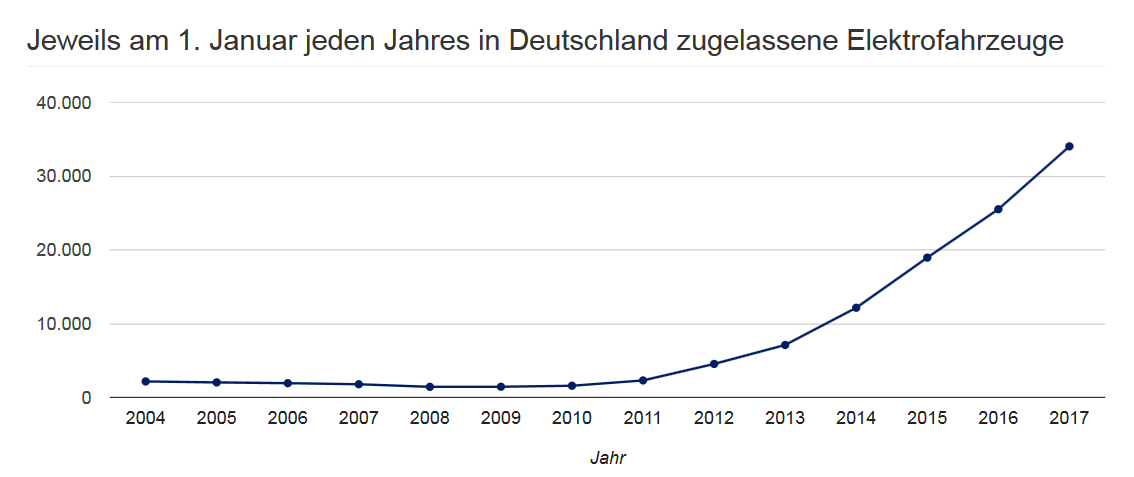
\includegraphics[width=14cm]{Efahrzeuge_Deutschland_2004_2017}
		\caption{Zugelassene E-Fahrzeuge in Deutschland von 2004 bis 2017 \cite{KBA_EAutos_Zulassungen} }
		\label{Abb:Efahrzeuge_Deutschland_2004_2017}
	\end{figure}
	
% Fördermittel
	Ein Flaschenhals bei der Elektrifizierung des automobilen Individualverkehrs ist die geringe Verfügbarkeit von Ladepunkten, weshalb der Ausbau der Ladeinfrastruktur durch Fördermittel des Bundesministeriums für Umwelt, Naturschutz, Bau und Reaktorsicherheit (BMUB) und des Bundesministeriums für Verkehr und digitale Infrastruktur (BMVI) begünstigt wird.\cite{BMVI_Frderrichtlinie_Ladeinfra}\\
% Momo: man braucht Ladepunkte um die Versorgung für die Autos zu gewährleisten - da könnts hacken bei laien

	\subsection{Projekt Energieverbundinsel}
		Auf Gebäude C der Hochschule Mannheim ist eine PV-Anlage mit einer Peakleistung von 20,145 kWp installiert mit einem durschnittlichen Jahresertrag von ca. 20.000 kWh. \\  %NOTE REF CITE XYZ
        % Der elektrische Verbrauch der gesamten Hochschule liegt bei ca. XYZ kWh pro Jahr.\\
		
		Im Sommersemester 2015 wurde im Rahmen einer Studienarbeit an der Hochschule Mannheim erstmalig ein Konzept für das Projekt Energieverbundsystem \glqq Energieinsel Mannheim\grqq \space erstellt. Mit beispielhaften Erzeuger- und Verbrauchersystemkomponenten wird eine Energieflussberechnung durchgeführt. Die betrachteten Systemkomponenten sind ein PV-System mit 25 kW Peakleistung, eine Lithium-Batterie mit ca. 27,5 kWh Speicherkapazität und 80\% \ac{DOD} mit zwei parallelen bidirektionalen Wechselrichtern mit einer Gesamtleistung von ca. 10 kW, Ladeinfrastruktur für Elektrofahrzeuge mit ca. 10,3 kW maximaler Ladeleistung, ein Elektrolyseur zur Wasserstoffgewinnung und eine Brennstoffzelle.\cite{STA_Oliver_Kersten_2015}\\
%Momo: -STC ne erklärung oder ne cite zu welche conditionas das sind

		Im Wintersemester 2017/18 wurde im Rahmen einer Bachelorthesis angelehnt an die \ac{HOAI}, eine Grundlagenermittlung, Vorplanung und Entwurfsplanung für die \glqq Errichtung einer Energieverbundinsel mit teilautarker Ladeinfrastruktur für Elektrofahrzeuge\grqq \space  erstellt. Die maximal angenommene Ladeleistung für E-Fahrzeuge beträgt 50 kW. Das angesetzte Budget von 50.000 EUR wurde leicht überschritten.\cite{BA_Chris_Ong_2017}\\
		
		Die geplante Energieverbundinsel mit PV-Speicher und Pufferbatterie besitzt die Grundvoraussetzungen für eine smarte teilautarke Betriebsweise mit implementiertem \ac{EMS} für experimentelle Tests in der Praxis.
% Momo: Normalmensch könnte bei den Worten smart und micogrid hängen


\section{Aufgaben und Ziele}
	% (Was ist das Ziel Ihrer Arbeit? Welche Aufgaben sind im Einzelnen zum Erreichen dieses Ziels zu bearbeiten?)
	%Zum Besseren Verständnis sollte bereits hier eine grafische Darstellung des zu automatisierenden Systems bereitgestellt werden. 
	Mit dieser Thesis wird das Ziel verfolgt die Planung der Errichtung einer Energieverbundinsel mit teilautarker Ladeinfrastrukur weiter zu entwickeln. Dafür wird ein Konzept für ein Energiemanagementsystem erstellt mit einer Übersicht der notwendigen Systemanforderungen zur intelligenten Steuerung und Überwachung der Ladetechnik für E-Fahrzeuge und Pufferbatterien.\\
	
	Mithilfe simulierter Energieflussberechnungen für verschiedene Szenarien sollen Handlungsempfehlungen für die Dimensionierung und Betriebsweise der Energieverbundinsel gegeben werden. Hierzu werden theoretisch erreichbare Autarkiegrade für die Ladeinfrastruktur in Abhängigkeit von Ladeleistung, PV-Leistung und Kapazität der Pufferbatterie ermittelt. Für die Simulationen wird eine Testumgebung in Matlab-Code geschrieben, um die Untersuchung weiterer Szenarien zu erleichtern. \\
	
%	Für eine Optimierung von Kosten, Aufwand und/oder Umweltschäden werden verschiedene Alternativoptionen zu der in \cite{BA_Chris_Ong_2017} aufgestellten Entwurfsplanung vorgestellt. Hierfür werden u.A. verschiedene verfügbare Batterietechnologien für den Einsatz als stationäre Pufferbatterien verglichen. \\
	
%	Pflichtenheft:
%	\begin{itemize}
%		\item Vorgaben: Ladeleistung * 120 \% Reserve < 50 kW 
%		\item Vorgaben: 3 Autos, 2 Roller/Motorräder, 5 Bikes
%		\item Konzept Energiemanagement
%		\item Zentrale Monitoring- und Steuerungseinheit entwerfen (Welche Daten werden geloggt, wie aufbereitet, wie angezeigt, was kann gesteuert werden, welche Kommunikationstechnik wird verwendet)
%		\item Überblick Systemkomponenten
%		\item Energieflussberechnung, Prognose
%		\item Mögliche Abrechnungssysteme bewerten ???
%		\item Kostenreduktion, Alternativoptionen ???
%	\end{itemize}

% Weitere Möglichkeiten:
%		Teststation für Energie-/Lastenmanagement und Kommunikation im IoT mit Option zur Fahrbatterieentladung
%		Ladeanschlusstechnik in open source (Anwendung des XYZ Protokolls, s. Signalisierung Typ 2 bzw. „Configuration FF“ - PLC-basiertes Layer-1-Kommunikationsprotokoll über Combo Typ-2-Stecker )
%		ev. selbstgebautes Batterypack https://batterybro.com/pages/18650-battery-pack

	

%	Energieverbundinsel
%		Energieflüsse\\
%			- Bilanzierung, geschätzte/r Erzeugung/Verbrauch
%			- Monitoring (Momentanwerte, Tagesverläufe, Wochen-/Monats-/Jahreswerte)\\
%				- - PV-Anlage\\
%				- - Akkus\\
%				- - Temperatur \\
%				- - Ladeverbrauch\\
%				- - Restliche Hochschule\\
%			- Controlling\\
%				- - Akkus\\
%				- - Heizsystem für Akkus- und Ladegeräte\\		


%		Kostensenkung\\
%			Holz-/Metallcontainer\\
%			PV-Anlage statt hoher Stromrechnung\\
%			Größer angelegte Batterie\\
%			Heizsystem für Batterie \\
%			Abrechnungssystem basierend auf OCPP\\


			

\section{Aufbau der Arbeit}
%	Orientierung an HOAI Leistungsphasen(LP) 1 bis 3.
%	
%	LP1: \\
%		- Technische Grundlagen zu bestehenden Ladesystemen verschiedener Fahrzeugtypen, Batterietypen, PV-Anlagen.\\
%		- Bestandsaufnahme Fahrzeuge, Standortanalyse, Zielvorgaben, Definition Workflow\\
%	LP2:\\
%		- Auslegung der Anlage (Ladeleistung, Batteriekapazität/-leistung, etc.)\\
%	LP3:\\
%		- Entwurfsplanung, Modelle erstellen, mit Anbietern/Herstellern beraten, Kostenrechnung\\
	Der Arbeit vorangestellt sind ein Abstract, das Ziele und Ergebnisse der Arbeit zusammenfasst und ein Abkürzungsverzeichnis.\\
    
	Die eigentliche Thesis beginnt mit einer Einleitung in Kapitel \ref{Kap1}, in der das Problemumfeld, die Ausgangssituation, die Aufgaben und Ziele und der Aufbau der Arbeit beschrieben werden. In Kapitel \ref{Kap2} wird die Basis für den Hauptteil der Arbeit geschaffen. Neben den technischen Grundlagen und Rahmenbedingungen wird dort das methodische Vorgehen beschrieben.\\
	
	In der ersten Hälfte des Hauptteils, Kapitel \ref{Kap3}, wird das Konzept der Energieverbundinsel und ein zugehöriges Energymanagementsystem entworfen.	In der zweiten Hälfte des Hauptteils, Kapitel \ref{Kap4}, werden Randbedingungen für verschiedene Szenarien für Energieflussberechnungen der Energieverbundinsel festgelegt, die Funktionsweise eines programmierten Simulationstools vorgestellt und die Ergebnisse der simulierten Energieflüsse wiedergegeben.\\
	
    In Kapitel \ref{Kap5} werden die Simulationsergebnisse zusammengefasst, bewertet und Handlungsempfehlungen für die Dimensionierung und Betriebsweise daraus abgeleitet sowie ein Ausblick auf zukünftige Entwicklungen geschaffen. Die Ergebnisse der Arbeit und eine kritische Schlussbetrachtung werden in einem Fazit in Kapitel \ref{Kap6} zusammengefasst. \\
    
    Im Anschluss an die Kapitel finden sich Verzeichnisse für Literaturquellen, Tabellen, Abbildungen und Quellcodes. \\
	
    Im Anhang finden sich technische Spezifikationen wie z.B. Datenblätter, Rechenmethoden zur Ermittlung von PV-Ertragsleistungen anhand waagrecht auf den Grund treffender Globalstrahlungsdaten, eine Beschreibung des Smart Grid Architecture Model (SGAM) Frameworks und Codebeispiele der entwickelten Programme.
    
     % ... Mit Orientierumg am Smart Grid Architecture Model, welches in Anhang \ref{Kap:SGAM_aufbau} näher beschrieben wird
     %  ...wird eine Use Case Analysis für die Anwendung der Energieverbundinsel durchgeführt. Aufbauend auf der Usecase Analysis werden die für die Simulation notwendigen Funktionalitäten, Datenmodelle und Komponenten beschrieben. 
    
     % Externe Datei einbinden
\chapter{Grundlagen, Bestandsaufnahme und Vorgehen}
	\label{Kap2}
    Dieses Kapitel umfasst technische Grundlagen zu physischen Komponenten einer Energieverbundinsel mit PV-Anlage, Pufferbatterie und Ladeinfrastruktur sowie zu Standards des Energiemanagement in intelligenten Netzen. Zudem werden die Rahmenbedingungen der Hochschule für die Energieverbundinsel vorgestellt und zuletzt eine Beschreibung des methodischen Vorgehens gegeben.
%\section{Definitionen}
%	Globalstrahlung
%	diffuse Strahlung
%	Direktstrahlung


%\begin{tabular}{|c|c|c|}
%	\hline 
%	Symbol & Beschreibung & Einheit  \\ 
%	\hline 
%	 & Globalstrahlung & $\frac{kW}{m^2}$ \\ 
%	\hline 
%	 & diffuse Strahlung & $\frac{kW}{m^2}$ \\ 
%	\hline 
%	 & Direktstrahlung & $\frac{kW}{m^2}$ \\ 
%	\hline 
%	 & Test für die Autoskalierung der Tabelle ................... &  \\ 
%	\hline 
%	&  &  \\ 
%	\hline 
%\end{tabular} 

	
\section{Technische Grundlagen}
	\subsection{Photovoltaik}
		\label{Kap:PV}
		Photovoltaikmodule, auch Solarmodule genannt, sind elektrisch in Reihe geschaltete Photovoltaikzellen, auch Solarzellen genannt, und meist zusätzlich mit Rahmen und Verglasung ausgestattet. Die Zellen bestehen aus einem Halbleitermaterial und wandeln durch den Photoelektrischen Effekt kurzwellige Strahlungsenergie in elektrische Energie um. An den PV-Zellen liegt unter Bestrahlung Gleichspannung an.\\
		
		PV-Zellen werden in der Regel nach Materialart und -stärke kategorisiert. Am häufigsten sind Siliziumzellen, welche es in monokristalliner, polykristalliner, mikrokristalliner oder amorpher Ausführung gibt. Selten gibt es auch mehrschichtige Ausführungen als Tandem-Solarzelle. Abb. \ref{Abb:Vgl_PV_eta} im Anhang stellt die Entwicklung der Wirkungsgrade verschiedener Arten von PV-Zellen von 1975 bis 2017 dar.\\
		
		Die Peakleistung $P_p$, mit der Einheit $Wp$, gibt die Ausgangsleistung der PV-Anlage in $W$ bezogen auf normierte Bedingungen, den \ac{STC}, an. Die STC sind wie folgt definiert:
		\begin{itemize}
			\item Einstrahlungsstärke $G_{STC}$ von $1000 \frac{W}{m^2}$ in Modulebene
			\item Temperatur der Solarzelle $25 ^{\circ} C$ konstant
			\item Strahlungsspektrum AM 1,5 global; DIN EN 61215, IEC 1215, DIN EN 60904, IEC 904 
		\end{itemize}
		AM steht für den Begriff Air Mass, wobei die Zahl für den Faktor an Wegstrecke durch die Atmosphäre in Relation zur Atmosphärenhöhe bezeichnet. Im Winter ist dieser Wert aufgrund eines niedrigeren Einstrahlungswinkels höher. Der Weg durch die Atmosphäre verändert das Spektrum der Globalstrahlung, daher die Bezeichnung \glqq global \grqq. In Anhang \ref{Kap:PV_global} ist eine Methode zur Ermittlung des PV-Ertrags anhand der GLobalstrahlung für ebene und geneigte Flächen beschrieben.\\
		
		PV-Anlagen werden über einen Wechselrichter mit dem Wirkungsgrad $\eta_{WR}$ ans elektrische Netz angeschlossen, der den DC-Strom in 230 V, 50 Hz AC-Strom umwandelt. Mithilfe eines Smartmeters kann die Energieerzeugung gemessen und mit zeitlicher Zuordnung gespeichert werden.


		
	\subsection{Akkumulatoren}
   	\label{Kap:Akkus}
		Akkumulatoren, auch Akkus genannt, sind elektrochemische, wiederaufladbare Energiespeicher, die vor allem in mobilen Geräten als Energiequelle dienen und in der Regel aus mehreren zusammengeschalteten Akku-Zellen bestehen. Je nach Einsatzbereich wird zwischen den folgenden zwei Typen von Akkus unterschieden: \\

		\textbf{Pufferbatterien} dienen der Versorgung elektrischer Schaltungen. Sie können zum Beispiel eine \ac{USV} gewährleisten und Regelleistung bereitstellen, um fluktuierende Erzeugung und Verbrauch insbesondere bei Inselanlagen auszugleichen. \\
		
		\textbf{Traktionsbatterien} dienen dem Antrieb von Elektrofahrzeugen.
		
	\subsubsection{Speicherkapazität, State of Charge (SoC) und Ladeleistung eines Akkus}
		Bei der Speicherkapazität eines Akkus muss zwischen verschiedenen Kapazitäten differenziert werden, der theoretisch verfügbaren, brutto und netto Kapazität $W_{theo}$, $W_{brutto}$ und $W_{netto}$. Zwischen der theoretisch verfügbaren und der praktisch genutzten Kapazität gibt es, wie in Abb. \ref{Abb:kap_theo_brutto_netto} dargestellt, zwei Sicherheitsbuffer, wobei diese nicht unbedingt symetrisch vom Minimum und Maximum her angelegt sein müssen. Der erste Buffer $W_{b1}$ dient der Betriebssicherheit, damit keine zu niedrigen Zellspannungen und durch Tiefenentladung bedingte Kurzschlussbrände sowie keine zu hohen Zellspannungen, wegen Überladung auftreten. Der zweite Buffer $W_{b2}$ dient der Optimierung der Akkulebensdauer.\\
		
					\begin{figure}[h]
						\centering
						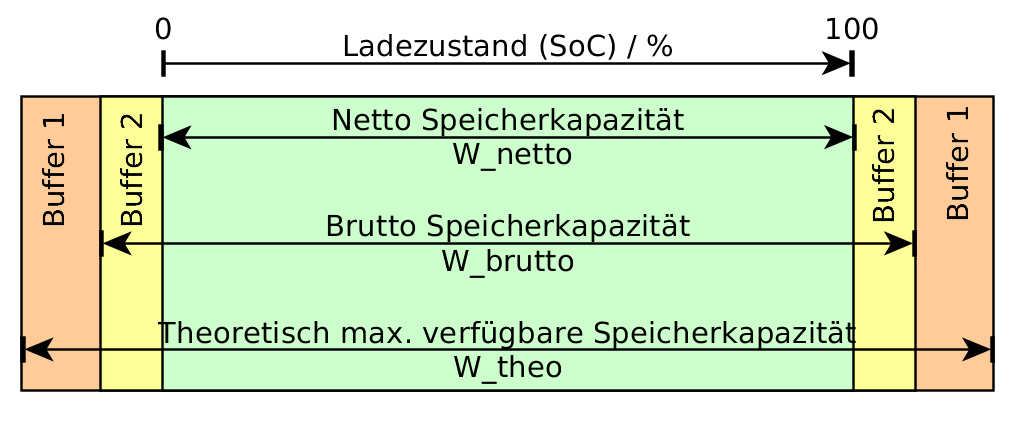
\includegraphics[width=14cm,height=5cm]{Speicherkap_theo_brutto_netto1}
						\caption{Speicherkapazitäten eines Akkus: \\
								Netto Speicherkapazität $W_{netto}$ (grün)\\
								Brutto Speicherkapazität $W_{brutto}$ (grün + gelb) \\
								Theoretisch max. verfügbare Speicherkapazität  $W_{theo}$ (grün + gelb + orange)}
						\label{Abb:kap_theo_brutto_netto}
					\end{figure}
		
		$W_{theo}$ ist die elektrochemisch, theoretisch verfügbare Kapazität eines Akkus.\\
		
		$W_{brutto}$, die brutto Speicherkapazität, ist die vom Zellhersteller freigegebene Kapazität und entspricht: $W_{brutto} = W_{theo} - W_{b1} $ \\
		
		$W_{netto}$, die netto Speicherkapazität, ist die vom Endprodukthersteller freigegebene Kapazität und entspricht: $W_{netto} = W_{brutto} - W_{b2} = W_{theo} - (W_{b1}+W_{b2})$ \\
		
		Der \ac{SoC} gibt an, wie viel Energie im Akku $W_{akku}$ bezogen auf seine netto Kapazität geladen ist: \\ $ SoC = \frac{W_{akku}}{W_{netto}}$ \\
		
		Die von einem Ladeanschluss maximal angegebene Leistung entspricht der maximalen brutto Ladeleistung $P_{brutto}$, die für den Ladevorgang maximal verbraucht werden kann. Der Akku wird dabei effektiv nur mit $P_{netto} = P_{brutto} * \eta_{charge}$ geladen, wobei $\eta_{charge}$ der Ladewirkungsgrad ist. Dieser ist das Produkt aus Wirkungsgrad des Akkus beim (Ent-)Laden und dem Wirkungsgrad des verwendeten Ladereglers. Es ist anzumerken, dass sich der Wirkungsgrad von Ladevorgängen zu dem von Entladevorgängen unterscheiden kann.\\
		
		 
%		Wichtige Kenngrößen von Akkus sind unter Anderem der \ac{SoC}, welcher den Ladezustand in Relation zum vollgeladenen Zustand angibt und der \ac{SoH}, welcher den maximal erreichbaren \ac{SoC} einer Batterie relativ zum maximal erreichbaren \ac{SoC} unter idealen Konditionen ohne Alterung angibt.  \\		
		

			
					
	\subsubsection{Batterieeigenschaften und Anforderungen}
		Akkus unterscheiden sich unter anderem durch die folgenden Merkmale von einander: Speicherkapazität, Energiedichte, Ladeleistung, Ladewirkungsgrade, ideale Temperaturbereiche für Be-/Entladung bzw. Lagerung, Zyklenfestigkeit (Lebensdauer) in Abhängigkeit der Entladetiefe (\ac{DOD}), Arbeits- und Transportsicherheit, Produktions- und Entsorgungsbedingungen, Ressourcenverfügbarkeit, mögliche Recyclinggrade, Umweltverträglichkeit sowie die Kosten für Anschaffung und Installation. \\
		
		

			
		
		\subsubsection{Batterietechnologien im Vergleich}
		%			\begin{figure}[h]
		%				\centering
		%				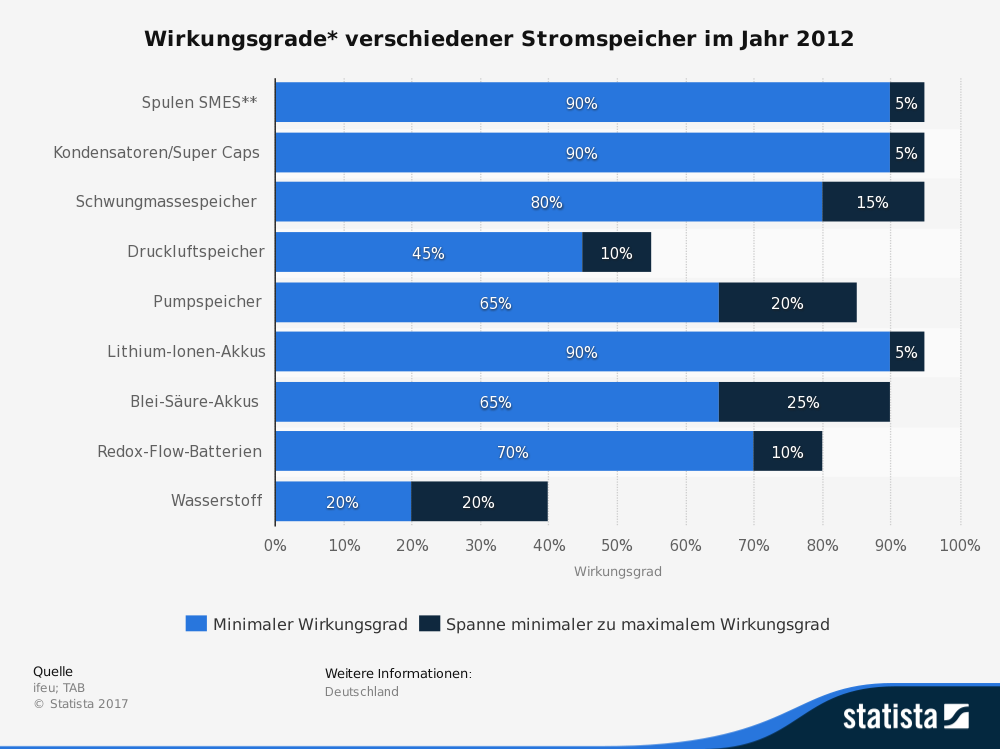
\includegraphics[width=14cm]{Batterietypen_Wirkungsgrade}
		%				\caption{Vergleich der Wirkungsgradspannbreite verschiedener Batterietechnologien im Jahr 2012 \cite[S.7]{AEE_ReNews_Strompseicher_2012} [Quelle XYZ iFEU, TAB, 2009] bzw. Renews AEE S.7}
		%				\label{Abb:Vgl_Batterien_eta}
		%			\end{figure}			
			In diesem Kapitel werden drei Speichertechnologien näher betrachtet.
			\begin{itemize}
				\item Bleisäureakkus, aufgrund dem weit verbreiteten Einsatz als Starterbatterien, Heimspeicher und für die \ac{USV}
				\item Lithiumakkus, aufgrund dem weit verbreiteten Einsatz in E-Fahrzeugen, mobilen Geräten und steigendem Gebrauch als Heimspeicher
				\item Bleikristallakkus, aufgrund der Temperaturfestigkeit, Langlebigkeit und Umweltverträglichkeit bei ähnlichem Preis wie Lithiumakkus
			\end{itemize}
			
			In Tabelle \ref{Tab:Vgl_Batterietechnologien} werden die Daten aus \cite{Comparison_Batteries_2015} zusammengefasst und um die Angaben der Wirkungsgrade und der geschätzten Kosten ergänzt. Die Kosten berücksichtigen nur die Batteriepreise ohne Ladetechnik. Zudem wurde die Zyklenfestigkeit von Bleikristallakkus, um die Herstellerangaben ergänzt, sowie die fehlenden Vorzeichen bei den Temperaturangaben in \cite{Comparison_Batteries_2015} korrigiert. Die Primärquelle ist nicht mehr verfügbar. Der angegebene Temperaturbereich entspricht mit korrigierten Vorzeichen den Entladetemperaturen anderer Quellen wie \cite{BATTUni_Temperatur}.\\ 
			
			Vertraut man den wenigen Herstellerangaben, so bieten Bleikristallakkus im stationären Einsatz als Pufferbatterie einen deutlichen Vorteil gegenüber Lithiumakkus oder herkömmlichen Bleisäureakkus. Es findet sich frappierender weise nur ein einziger Hersteller namens Betta Batteries, der seit 2009 die patentierte Lead Crystal(R) Technologie einsetzt, obwohl es bereits seit 1979 Patente für den Einsatz von Bleikristallakkus gibt. \cite{patent1}\cite{patent2} 
			
			%			Patente von 1977:
			%				http://www.freepatentsonline.com/4143216.html
			%				https://www.google.com/patents/US4140589
			
			\begin{table}[h]
				\centering
				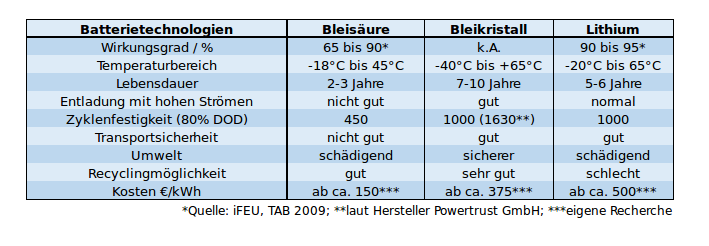
\includegraphics[width=14cm]{Vgl_Batterietechnologien}
				\caption{Vergleich von Batterien auf Basis von Bleisäure, Bleikristall und Lithium; \cite{Comparison_Batteries_2015}, *\cite[S.7]{AEE_ReNews_Strompseicher_2012}}
				\label{Tab:Vgl_Batterietechnologien}
			\end{table}

% Logisch:
%		\textbf{Sicherheitshinweis:} \\ 
%		Bei Intebetriebnahme von Pufferakkus sind ... Um die Betriebssicherheit zu gewährleisten müssen notwendige Brandschutzbedingungen beachtet werden. Je nach Akkutyp können sonst Kurzschlussbrände und Ausgasung von explosivem Wasserstoff aufgrund von Hydrolyse vorkommen. \\
	
	\subsection{Ladesysteme für E-Fahrzeuge}
		\label{Kap:Ladesysteme}
		Die internationale Norm IEC 61851 spezifiziert die elektrische Ausrüstung von Elektro-Straßenfahrzeugen u.A. konduktive Ladesysteme. 
		
		\subsubsection{E-Autos}
			\paragraph{Lademodi}
				Traktionsbatterien können sowohl mit Wechsel- als auch Gleichstrom beladen werden. In Tabelle \ref{Tab:Vgl_Ladesysteme_EAuto} werden verschiedene Lademodi für Elektro-Autos gezeigt. Die Lademodi eins bis vier für kabelgebundene Ladungen sind in der internationalen Norm IEC 62196 (in Deutschland als DIN EN 62196 gültig) zusammen mit den dazugehörigen Steckertypen spezifiziert. Für den Lademodus 5 mit kabelloser induktiver Ladung gibt es derzeit noch keine einheitliche Norm.


			\paragraph{Steckertypen}
				In Tabelle \ref{Tab:Vgl_Steckervorrichtungen} sind die üblichen Steckertypen zum Laden von E-Fahrzeugen mit Grafiken zur Bauform, Übertragungsart, mögliche Ladeleistungen und -ströme aufgelistet.
				
				\textbf{Steckertypen für AC-Ladungen} In der Norm IEC 62196-2 werden die folgenden drei verschiedene AC-Stecker normiert und mit "Typ 1" bis "Typ 3" bezeichnet. 
				
				\begin{itemize}
					\item Typ 1: SAE-J1772-2009
					\item Typ 2: Mennekes Stecker, deutscher Standard
					\item Typ 3: EV-Plug-Alliance Stecker, Erweiterung von Typ 2 mit Shuttern; findet keine Verwendung
				\end{itemize}
				
				\textbf{Steckertypen für DC-Ladungen} sind derzeit meistens eines der folgenden weltweit vorherrschenden Systeme.
				
				\begin{itemize}
					\item Combo 1, CCS (USA), basierend auf Typ 1
					\item Combo 2, CCS (Europa), basierend auf Typ 2, deutscher Standard
					\item CHAdeMO in Japan und weltweit \cite{IEC_CHAdeMO}
					\item Tesla Supercharger (exklusiv für Fahrzeuge der Marke Tesla Motors), Typ 2 modifiziert
				\end{itemize}
				
				Combo 1, Combo 2 und CHAdeMO sind durch die internationale Normen der IEC spezifiziert. \\
				
				Die beiden DC-Steckertypen \ac{CCS} Combo 1 und Combo 2 kommunizieren über Powerline Connectors und basieren wie in der Tabelle \ref{Tab:Vgl_Steckervorrichtungen} im Anhang zu erkennen auf den AC-Steckern vom Typ 1 und Typ 2. Dadurch sind Autos mit CCS-Anschluss für die AC-Stecker kompatibel. Die Kommunikation bei CHAdeMO funktioniert über einen seperaten CAN-Bus. \cite{Emobility_StatusQuo_2016} \\ 
				
				Durch die EU-Richtlinie für den Aufbau der Infrastruktur für alternative Kraftstoffe gilt europaweit Typ 2 als Standard für AC-Ladungen über 3,6 kW und Combo 2 für DC-Ladungen über 22 kW. \cite{EU_Aufbau_Infrastruktur} Mit Inkrafttreten der Ladesäulenverordnung in Deutschland wurden die Ladestecker vom Typ 2 zum Standard des AC-Ladens und die Ladestecker vom Typ Combo 2 entgegen der EU-norm auch bei DC-Ladepunkten unterhalb von 22 kW zum Standard des DC-Ladens. \cite{BMJV_LSV} \\


				
% NOTE: Interessant, aber unwichtig, da inkombatibel mit Fahrzeugen		
%			\begin{figure}[h]
%				\centering
%				\includegraphics[width=6cm]{AC_DC_Steckervorrichtung_Typ2.jpg}
%				\caption{Vergleich verschiedener Steckervorrichtungen basierend auf Typ 2 für AC- und DC-Ladung. Nur die oberste und unterste Kontaktbelegung sind normiert.}
%				\label{Abb:Vgl_Steckervorrichtungen_Typ2}
%			\end{figure}			
%			
%			[Quelle für's Bild: %http://www.mennekes.de/uploads/media/MENNEKES_Medieninformation_-_Ladesteckvorrichtungen_Typ_2_f%C3%BCr_AC_und_DC_Ladung_02.pdf 
%			]
			
			
			\paragraph{Ladeinfrastruktur für E-Autos in Deutschland}
				In Abb. \ref{Abb:BDEW_Anzahl_Ladepunkte} ist die Entwicklung der E-Mobilität in Deutschland, gemessen an der Anzahl an öffentlich zugänlichen Ladepunkten und zugelassenen Elektrofahrzeugen dargestellt.\\
					
				\begin{figure}[h]
					\centering
					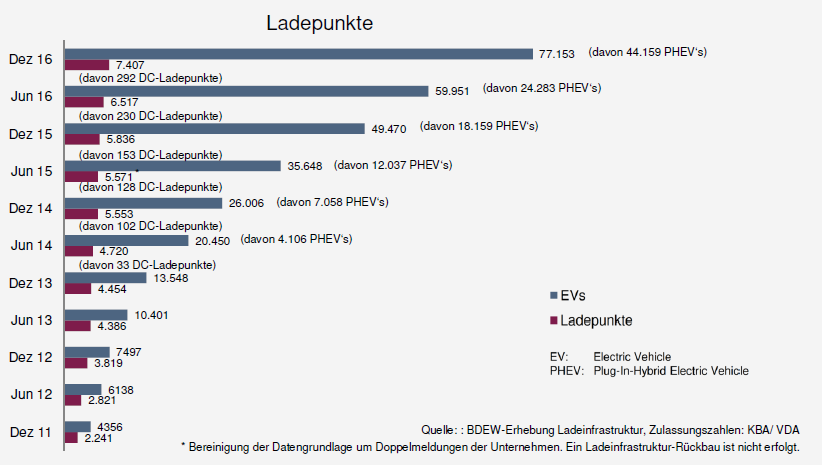
\includegraphics[width=14cm]{BDEW_Anzahl_Ladepunkte}
					\caption{Anzahl der Ladepunkte in Deutschland und EVs, Dez. 2011 bis Dez. 2016 \cite{BDEW_Anzahl_Ladepunkte}}
					\label{Abb:BDEW_Anzahl_Ladepunkte}
				\end{figure}	
			
				An den 7.407 öffentlichen Ladepunkten in Deutschland, Stand 31.12.16, sind folgende Abrechnungssysteme installiert, wobei je Ladepunkt mehrere Abrechnungssysteme möglich sind. \cite{BDEW_Anzahl_Ladepunkte} \\
				
				\begin{itemize}
					\item 4.801 RFID-Karte (rel. 65\%)
					\item 3.203 Smartphone App (rel. 43\%)
					\item 1.155 Plug'n'Charge (rel. 16\%)
					\item 1.428 Sonstige (rel. 19\%)
				\end{itemize}
			
			\subsubsection{E-Motorräder und E-Roller}
				E-Motorräder können mit dem entsprechenden Ladezubehör an jeder herkömmlichen Schuko-Steckdose geladen werden. Eine öffentliche Ladeinfrastruktur mit Schnelladepunkten ist derzeit noch nicht verfügbar.
				
				Hersteller für Elektro-Motorräder und Zubehör wie Zero Motorcycles bieten auch externe Schnelladegeräte wie den Charge Tank mit 6 kW Ladeleistung als Ergänzung zum internen Ladegerät mit ca. 1,5 kW ihrer Fahrzeuge an. Dieser kann an Level-2-Ladestationen, mit Steckertyp 2, angeschlossen werden.[Quelle] 
			
%			Beispielfahrzeuge:
%			QvR VR One 
%				https://www.adac.de/_mmm/pdf/ADAC%20Fahrberichte%20_%20QvR_91kb_122015.pdf
%			Vectrix VX-1 LI+ 
%				https://www.adac.de/_mmm/pdf/ADAC%20Fahrberichte%20_%20ZeroVectrix_92kb_122013.pdf
%			ZERO DS 
%				https://www.adac.de/_mmm/pdf/ADAC%20Fahrberichte%20_%20Zero_91kb_122014.pdf
			
			
			\subsubsection{E-Bikes und Pedelecs}
				Fast alle Elektrofahrräder können mit Ladekabel und Netzteil an einer herkömmlichen 230 V Schuko-Steckdose geladen werden.\\
				
				Die häufigsten Formen von Fahrradladestationen sind:
				\begin{itemize}
					\item Fahrradständer mit angebrachten Steckdosen
					\item Abschließbare Akkuschränke mit im Innern angebrachten Steckdosen
					\item Ladesäule mit angebrachten Steckdosen 
					\item Ladesäule mit eigenem Kabelsystem (z.B. von bike-energy)
				\end{itemize}
				
				% Bike energy 
				% http://www.bike-energy.com/


		\subsection{Energiemanagement im intelligenten Stromnetz}
		\label{Kap:Grundlagen_Energiemanagement}
		% Einleitung
		In diesem Kapitel wird das Konzept und das Ziel von Energiemanagement beschrieben und es werden verschiedene Standards für Smart Grid Anwendungen vorgestellt. 	
		
		\subsubsection{Definition Energiemanagement, Energymanagementsystem (EMS), Smartgrid}
		% Definition Energiemanagement
			\glqq Energiemanagement ist die Kombination aller Maßnahmen, die bei einer geforderten Leistung einen minimalen Energieeinsatz sicherstellen. Es bezieht sich auf Strukturen, Prozesse und Systeme sowie auf menschliche Verhaltensweisen und -änderungen.\grqq \cite{Def_Energiemanagement} Damit umfasst Energiemanagement die Planung und den Betrieb energietechnischer Verbrauchs- und Erzeugungseinheiten, im folgenden \ac{CPS}-units genannt. \\ 
			
		% Definition Energiemanagementsystem
			Ein \ac{EMS} dient der systematischen Erfassung, Kommunikation und Regelung von Energieflüssen z.B. durch Smart Metering und der automatisch auf einander abgestimmten Steuerung mehrerer Geräte.\\
			
		% Definition Smart Grid
			Ein intelligentes Stromnetz (englisch Smart Grid) ist eine Form eines \ac{EMS}. Ein Smart Grid umfasst die kommunikative Vernetzung und Steuerung von CPS-units, wobei abhängig von den Ausmaßen des Smart Grids auch von Microgrids und Nanogrids gesprochen wird. Eine normierte Definition der Bezeichnungen gibt es (noch) nicht. \\
			
		\subsubsection{Ziele von und Ansätze für Energiemanagement}
		% Ziele
			Die Energieflüsse können hinsichtlich verschiedener Gesichtspunkte optimiert werden. Ziele können u.A. sein:
			\begin{itemize}
				\item Energiekostensenkung
				\item Ressourcenschonung
				\item Verbesserung der Netzstabilität und Versorgungssicherheit
				\item Autarkiegraderhöhung durch bessere Nutzung eigenproduzierter Energie
			\end{itemize}

		% Ansätze
			Smart Grids können abhängig von der Architektur u.A. die folgenden Möglichkeiten für Energiemanagement bereit stellen:
			\begin{itemize}
				\item Smart Metering (Erfassung und Kommunikation von Messdaten durch intelligente Zähler)
				\item Bereitstellung von Regelleistung (durch Regelung oder Abschaltung von CPS-unit wie sz.B. Pumpspeicherkraftwerke, konventionelle Dampfkraftwerke, BHKWs, Biogas- und Müllverbrennungsanlagen, Batteriespeicher, Lüftungs- und Kühlsystemen, elektrischen Heizsystemen)
				\item Automatisches \ac{DSM} durch Einsatz von \ac{GFA} Controllern zur Primärregelung der Netzfrequenz ohne zentrale Steuerung und ohne Kommunikation mit anderen CPS-units
			\end{itemize}

% GFA Quelle:
%				http://ieeexplore.ieee.org/document/6732970/?reload=true&tp=&arnumber=6732970&refinements%3D4291944246%26ranges%3D2014_2015_p_Publication_Year%26queryText%3DFPGA
% https://www.researchgate.net/publication/224188933_Frequency_waves_Grid_Friendly_Appliances_and_geographic_limits_in_a_smart_grid



			% Schema mit Hardwarekomponenten, verschiedenen Bussystemen und Steuereinheit
			
			\subsection{Smart Grid Architecture Model (SGAM) Framework}
				Das \ac{CENELEC} hat einen Bericht der Smart Grid Coordination Group und Reference Architecture
				Working Group veröffentlicht mit der Beschreibung des \ac{SGAM} Framework, einem interoperablen Modell für Smart Grid Architekturen. Ziel des SGAM ist es, aus verschiedensten Standards ein umfängliches, kompatibles, konzeptuelles Modell mit holistischem Ansatz als für alle Anwendungsfälle unabhängig von der angewandten Technologie zu erstellen. \cite{CENELEC_SmartGrid} \\
                
				Einige solcher sich teilweise überschneidender Standards sind beispielsweise die "German standardization roadmap E-Energy" des \ac{DKE}, die IEEE Standards IEEE SCC21 (Standards Coordinating Comittee on Fuel Cells, Photovoltaics, Dispersed Genreration, and Energy Storage), P2030 (Standard Interoperability Smart Grid Concepts) und die Framework und Roadmap for Smart Grid Interoperability Standards, das \ac{NIST EA Model}. \cite{DKE_SmartHome} \\ %NOTE: cite XYZ IEEE standards
				
				%NOTE: Warum werden einige dem SGAM zugrunde liegenden Standards aufgelistet?
				
				Der Aufbau des SGAM Frameworks wird ausführlich in Anhang \ref{Kap:SGAM_aufbau} beschrieben.
				
		

			\subsubsection{Open Gateway Energy MAnagement 2.0 (OGEMA 2.0)}
				\ac{OGEMA} 2.0 ist ein open source Software-Framework und dient als Programmierschnittstelle für Energiemanagement Anwendungen. Es ermöglicht die Realisierung von Energiemanagementsystemen für Gebäude, den industriellen Bereich und die Elektromobilität. Das Framework nutzt, wie in Abb. \ref{Abb:OGEMA_Aufbau} zu sehen ist, eine Java-Plattform und standardisierte Datenmodelle für verschiedenste Energieerzeuger, -verbraucher und -speicher. Die Software ist hardwareunabhängig und kann somit leicht an andere Plattformen adaptiert werden. \cite{OGEMA_Praes} \\
                
				Entwickelt wurde OGEMA mit Förderungen des Bundesministeriums für Wirtschaft und Energie von den drei Fraunhofer Instituten für Windenergie und Energiesystemtechnik (IWES), für integrierte Schaltungen (IIS) und für solare Energiesysteme (ISE). Derzeit gibt es verschiedene Projekte in denen Smart Grid Anwendungen mit OGEMA getestet werden, darunter eines in Mannheim. \cite{ogemamoma}
				
				\begin{figure}[h]
					\centering
					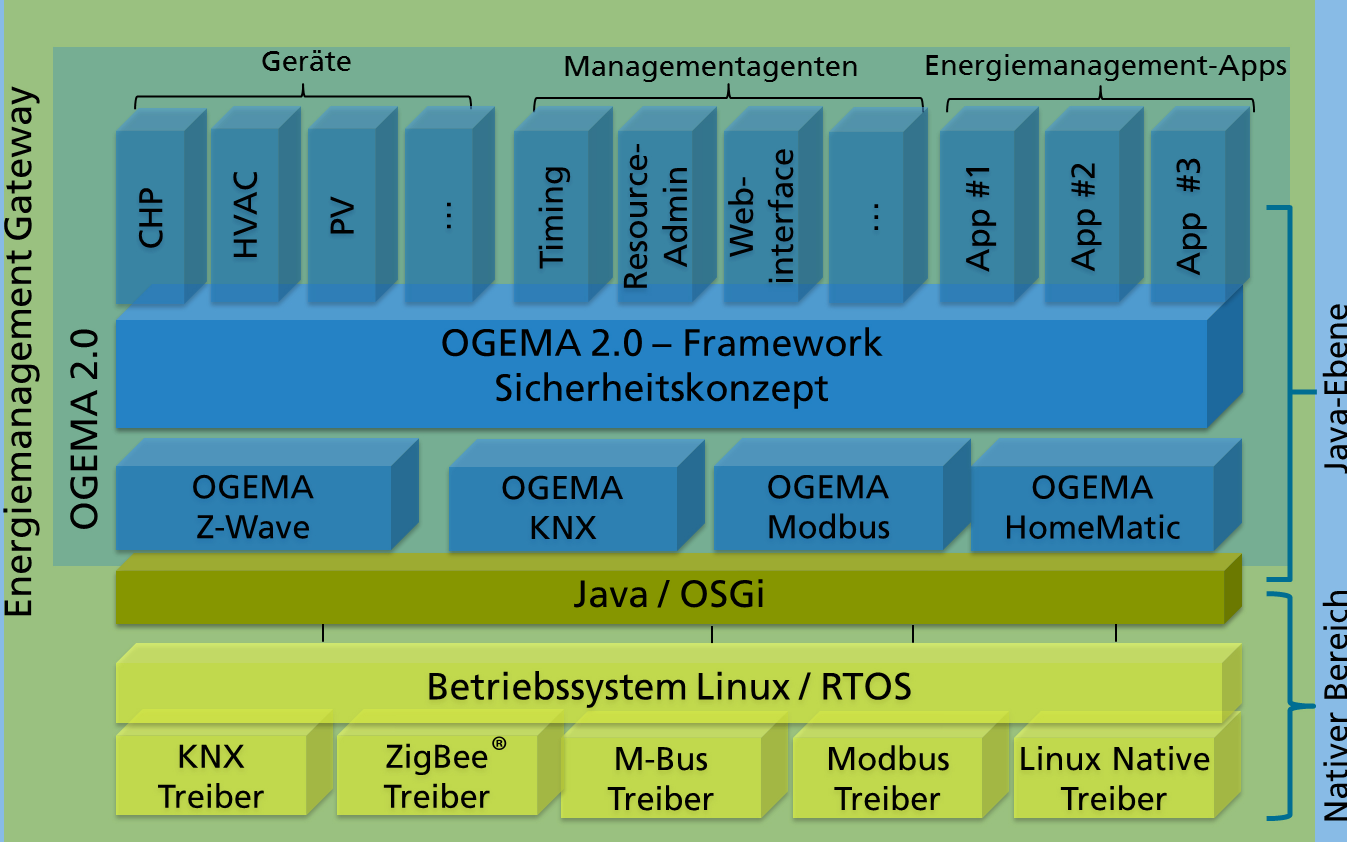
\includegraphics[width=14cm]{OGEMA}
					\caption{Modulare Baukastenstruktur von OGEMA \cite{OGEMA_Praes}}
					\label{Abb:OGEMA_Aufbau}
				\end{figure}			
	
%				Im Zuge dieser Bachelorarbeit war es nicht möglich das OGEMA 2.0 Demokit auf den Betriebssystemen Windows 7, Windows 10 und XUbuntu (s. Abb. \ref{Abb:OS_java_ubuntu}) zu starten.\\
				
%				Version des Betriebssystems und Javas unter XUbuntu: \\
%				Distributor ID:	Ubuntu \\
%				Description:	Ubuntu 16.04.4 LTS \\
%				Release:	16.04 \\
%				Codename:	xenial \\
%				openjdk version "1.8.0\_162" \\
%				OpenJDK Runtime Environment (build 1.8.0\_162-8u162-b12-0ubuntu0.16.04.2-b12)\\
%				OpenJDK 64-Bit Server VM (build 25.162-b12, mixed mode)\\
				
				
%				\begin{figure}[h]
%					\centering
%					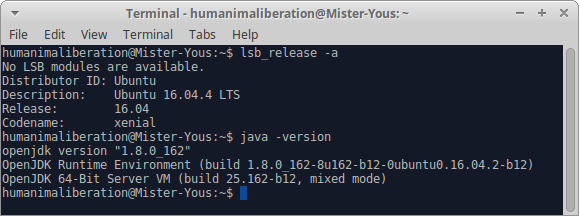
\includegraphics[width=14cm]{OS_java_ubuntu}
%					\caption{Version von Betriebssystem und Java der laufenden XUbuntu Distribution}
%					\label{Abb:OS_java_ubuntu}
%				\end{figure}			
				
				%NOTE XYZ Win 10 
				
%				https://www.energy-seeds.org/content/dam/energy-seeds/de/documents/22_2014-10-27_Energiesymposium_FhG-IIS-Heusinger_Flexible-Softwarplatforem-Energiemanagement.pdf



				
			\subsubsection{EEBUS und Smart Premises Interoperable Neutral-message Exchange (SPINE)}
				Das EEBUS Datenmodell ist Bestandteil internationaler Standards:
				
				\begin{itemize}
					\item CENELEC EN 50631 (Interoperable Connected Household Appliances) \cite{CENELEC}
					\item ETSI TS 103 410-1 SAREF4ENER (EU Framework SAREF; Smart Appliances REFerence) \cite{Etsi}
				\end{itemize}
							EEBUS ist trotz des Namens kein Bus-System, sondern ein offener Standard für eine Kommunikationsschnittstelle, die von jedem Gerät und jeder technischen Plattform unabhängig von Hersteller und Technologie genutzt werden kann. Somit ermöglicht EEBUS energietechnisch relevanten Geräten im \ac{IoT} in einer standardisierten Sprache für Steuerung und Management miteinander zu kommunizieren. \\ %Ev. auch wichtig ISA‐62443‐1‐4SecurityLifecycleundUseCases–auchbekanntalsISA 99


			
				
				Die zugrundeliegende Technik von EEBUS ist die Datenmodell-Spezifikation von \ac{SPINE} wie in Abb. \ref{Abb:EEBUS_Spec} im Anhang dargestellt. \\
				
				Entwickelt wird der EEBUS-Standard von dem 2012 gegründeten gemeinnützigen Verein EEBus Iniative e.V., der von Vertretern namenhafter Unternehmen aus der Industrie als auch des europäischen Komitees für elektrotechnische Normung CENELEC geleitet wird. Hervorgegangen ist EEBUS aus dem Projekt Smart Watts des Förderprogramms E-Energy, das vom Bundesministerium für Wirtschaft und Technologie (BMWi) und dem Bundesministerium für Umwelt, Naturschutz und Reaktorsicherheit (BMU) aufgelegt wurde.\\

				\paragraph{SPINE}
				\ac{SPINE} definiert Nachrichten und Verfahrensweisen nur auf der Anwendungsebene nach dem ISO-standardisierten \ac{OSI-Modell}. Das OSI-Modell beschreibt 7 Ebenen für die Kommunikation zwischen zwei Systemen, von der Anwendungsebene über die (optionale) Darstellungs- und (optionale) Sitzungsebene, über die Transport-, Vermittlungs- und Sicherungsebene zur Bitübertragungsebene. Abb. \ref{Abb:EEBUS_Spec} zeigt die Abgrenzung zur Transportebene. Es ist damit komplett unabhängig vom gewählten Transportprotokoll. In Abb. \ref{Abb:SPINE_SGAM_Layers} ist SPINE im \ac{HBAM}, eingeordnet, welches sich vom \ac{SGAM} ableitet. \\
				
				\begin{figure}[h]
					\centering
					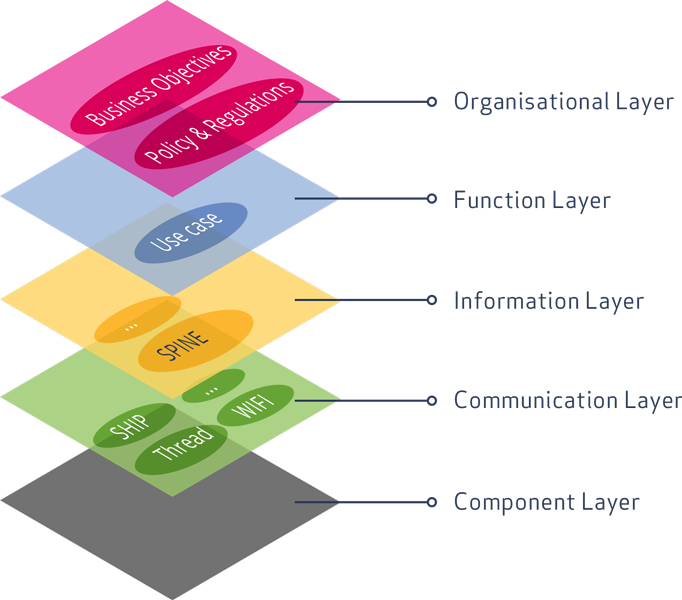
\includegraphics[width=8cm]{SPINE_SGAM_Layers}
					\caption{Einordnung von SPINE in das \ac{SGAM} sowie der daraus abgeleiteten \ac{HBAM} \cite{EEBUS_Web}}
					\label{Abb:SPINE_SGAM_Layers}
				\end{figure}			
				
				Die nach SPINE-Spezifikation normierten Datenmodelle sind interoperable und für verschiedene Protokolle und Übertragungswege nutzbar. Damit ist es beispielsweise mit WLAN oder KNX, welches in der Gebäudetechnik weit verbreitet ist, kompatibel. Mit entsprechenden Treibern müsste das SPINE-Datenmodell auch mit OGEMA-Anwendungen kompatibel sein.\\
				
				Das SPINE-Datenmodell umfasst Datensätze für Anwendungsfälle (use cases) mit Metadaten z.B. über die jeweiligen physikalischen und logischen Gerätetypen (device and entity type) und Funktionalitäten (features) sowie komplexe Klassen und Standard-Klassen mit konkreten Funktionen für die Steuerung der jeweiligen Geräte. \cite{EEBUS_Intro} \\

			\subsubsection{Open Charge Point Protocol (OCPP)}
				Das Protokoll OCPP definiert die Kommunikation zwischen Ladepunkt und Zentralsysten, nicht aber die verwendete Kommunikationstechnologie. Jede Technologie, die TCP/IP-Verbindungen unterstützt kann eingesetzt werden. Die verschiedenen Versionen sind aufgrund neuer Eigenschaften nicht unbedingt rückwirkend kompatibel. Im März 2018 kam die derzeit aktuelle Version 2.0 heraus. In der Version 1.5 und 1.6 gab es noch erhebliche Sicherheitsprobleme, die neben anderen in Kapitel \ref{Kap3} erwähnt werden. \cite{CCC} \cite{evsim} 
	
						
				
		\subsection{Autarkiegrad und Eigenverbrauchsanteil}
			Der Autarkiegrad eines Systems kann hinreichendes Bewertungskriterium zur Optimierung dessen Energieflüssen sein. Er gibt den relativen Anteil der verbrauchten Energiemenge im System an, die innerhalb des Systems erzeugt werden kann. Ein Autarkiegrad von 100\% bedeutet demnach ein energieautarkes System, welches die Menge an benötigter Energie selbst erzeugen kann.\\
			
			$Autarkiegrad = \frac{Erzeugte\, Energie\, im\, System}{Verbrauchte \,Energie\, im\, System}$ \\
			
			Der Eigenverbrauchsanteil hingegen gibt den relativen Anteil der von einem System erzeugten Energiemenge an, die darin selbst verbraucht wird. Ein Eigenverbrauchsanteil von 100\% bedeutet nur, dass die gesamte erzeugte Energie des Systems von diesem selbst verbraucht wird. \\
			
			$Eigenverbrauchsanteil = \frac{Erzeugte\, Energie\, im\, System,\, die\, im\, System\, verbraucht\, wird}{Erzeugte\, Energie\, im\, System}$
			
			

						
\section{Rahmenbedingungen}
	\label{Kap:Rahmenbedingungen}
	\subsection{Standortanalyse}
	Abbildung \ref{Abb:Campusplan} zeigt den Campusplan der Hochschule Mannheim. Der Standort vor dem Hochspannungslabor, Gebäude F, für zwei Container der Energieverbundinsel wie in der Planung von Frau Ong vorgesehen, wurde von der Stadt abgelehnt. \cite{BA_Chris_Ong_2017} Die Ladesäule vor der Bibliothek, Gebäude L, wurde abgebaut und dafür wurde zwischen Gebäude B und Grünfläche eine Ladesäule mit einem einzelnen Stecker des Typ 2 und einer maximalen ladeleistung von 22 kW errichtet. Ein weiterer Ausbau der Ladeinfrastruktur ist gegenwärtig (im Mai 2018) noch nicht geplant.
    
		\begin{figure}[h]
			\centering
			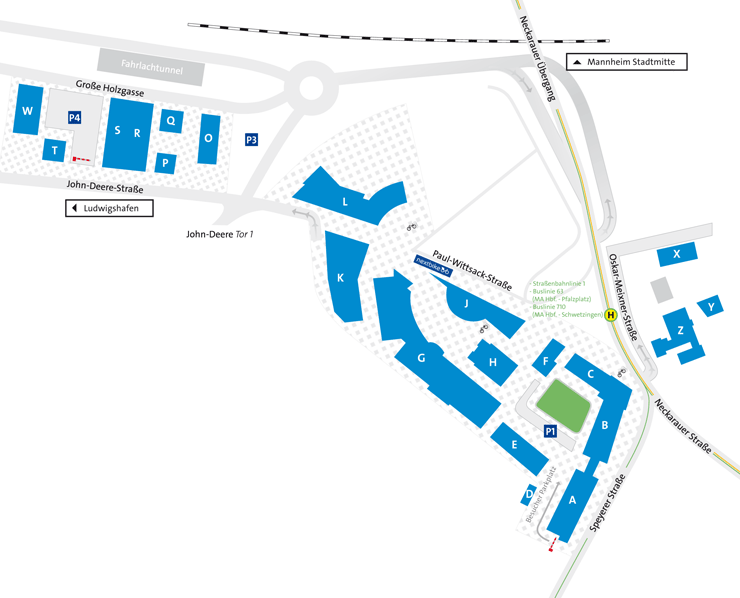
\includegraphics[width=0.9\textwidth]{campusplan_edit}
			\caption{Campusplan der Hochschule Mannheim \cite{HS_Campusplan}}
			\label{Abb:Campusplan}
		\end{figure}			

	\subsection{E-Fahrzeuge}
		\label{Kap:Fahrzeuge}
		Die Hochschule Mannheim besitzt zwecks Forschung und Fortbewegung für Mitarbeiter*innen eine Reihe verschiedener E-Fahrzeuge. Diese sind in Tabelle \ref{Tab:EFahrzeuge_Liste} mit einer Typenbezeichnung, der Batteriekapazität und den verfügbaren Ladeoptionen aufgelistet. Die Fahrzeugflotte der Hochschule Mannheim ist nicht repräsentativ für die E-Fahrzeuge im deutschen Straßenverkehr, werden vorraussichtlich aber den Großteil der zu ladenden Vehikel in der Energieverbundinsel darstellen.  \\
		
		Neben den Hochschulfahrzeugen werden zusätzlich der Zoe Z.E.40 von Renault, der i3 von BMW und der fortwo von Smart mit optionalem 22kW-Bordlader als Referenzautos angegeben. Der Zoe ist in Deutschland das E-Auto mit den meisten Neuzulassungen 2017. Der i3 liegt auf Platz 2 und war  im Vorjahr auf Platz 1 der Neuzulassungen. Gegenüber dem Stromos besitzen beide Fahrzeuge eine höhere Batteriekapazität und mögliche Ladeleistung. \cite{EAutos_Ranking}
		
		\begin{table}[h]
			\centering
			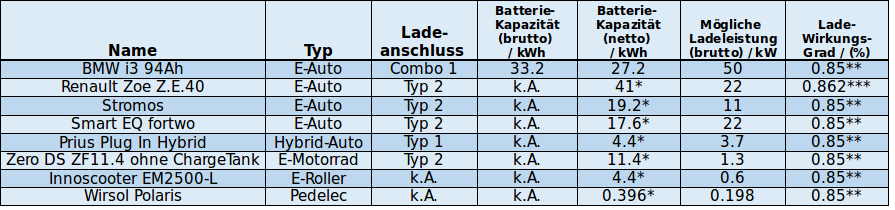
\includegraphics[width=14cm]{EFahrzeuge_Liste}
			\caption{Liste verschiedener E-Fahrzeuge mit Kenndaten nach Herstellerangaben\cite{spec_i3} \cite{spec_i3eng} \cite{spec_zoe} \cite{spec_stromos} \cite{spec_smart} \cite{spec_prius} \cite{spec_zero} \\ *Annahme: Herstellerangabe ist brutto Kapazität mit 85\% netto Kapazität
			\\ **eigene Schätzung
			\\ ***Mittelwert von Messungen eines Fahrzeugnutzenden \cite{spec_zoeeta}}
			\label{Tab:EFahrzeuge_Liste}
		\end{table}			
		
    \subsection{Kenndaten der PV-Anlage}
		In Tabelle \ref{Tab:PV_kenndaten} sind die Kenndaten der PV-Anlage und des PV-Wechselrichters (PV-WR) auf Gebäude C der Hochschule Mannheim aufgelistet. Die Kenndaten sind den Herstellerspezifikationen im Anhang \ref{Kap:datasheet_pv_wr} entnommen. 
		
		\begin{table}[h]
			\begin{tabular}{|c|c|c|}
				\hline 
				 							& \textbf{Wert / Modellbezeichnung} & \textbf{Einheit} \\ 
				\hline 
				PV-Module 							& REC PE 265 Wp &   \\ 
				\hline 
				Peakleistung PV-Modul unter STC 	& 265 		& Wp \\ 
				\hline
				Wirkungsgrad PV-Modul unter STC 	& 16,1 		& \%  \\ 
				\hline 
				Modulfläche 						& 1,65 		& $m^2$  \\ 
				\hline 
				Anzahl PV-Module 					& 76 		& \\ 
				\hline  
				Peakleistung PV-Anlage unter STC	& 20,145 	& kWp  \\ 
				\hline 
				PV-Wechselrichter (PV-WR) 			& SAM STP 20.000 TL-þ30 & \\ 
				\hline
				Wirkleistung PV-WR 					& 14,09 	& kW\\
                									& (reduziert auf 70\%)   &\\ 
				\hline
				PV-WR: NA-Schutz 					& integriert &\\ 
				\hline
			\end{tabular} 
			\caption{Kenndaten der PV-Anlage auf Gebäude C der Hochschule Mannheim} %NOTE XYZ REF Anhang Datenblatt
			\label{Tab:PV_kenndaten}
		\end{table}
		
		
% NOTE: Fehlt noch:
%		Keine Verschattung
%		Modulausrichtung:
%		Modulneigung: Hälfte 7,72°, andere Hälfte -7,72°

		


		
	\subsection{Vorgaben bei der Dimensionierung}
		\label{Kap:Vorgaben}
		
		% Grundkonzept und Pmax der gesamten Ladeinfrastruktur
		Die Energieverbundinsel soll Lademöglichkeiten für 3 Autos, 2 Motorräder und 5 Fahrräder besitzen. Der Anschluss ans Hochschulnetz ist dabei auf eine verfügbare Leistung $P_{max}$ von maximal 50 kW + 20 \% Reserve begrenzt. Abbildung \ref{Abb:Netztopologie} zeigt den schematischen Aufbau der relevanten CPS-units in der Energieverbundinsel.\\

		Die Dimensionierung der Ladepunkte erfolgt unter Berücksichtigung von $P_{max}$ und den üblicherweise für E-Fahrzeugen ausgelegten Ladeleistungen (s. Kapitel \ref{Kap:Fahrzeuge}) mit den in Tabelle \ref{Tab:Ladepunkte} aufgelisteten Steckertypen und Anschlussleistungen. \\
        
		\begin{figure}[h] % Netztopologie
			\centering
			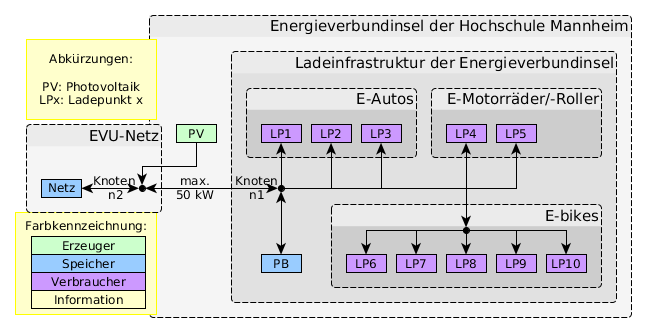
\includegraphics[width=14cm]{Netztopologie1}
			\caption{Geplante Netztopologie der Energieverbundinsel}
			\label{Abb:Netztopologie}
		\end{figure}		
			
		\begin{table}[h]
			\centering
			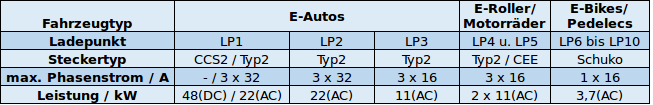
\includegraphics[width=14cm]{Ladepunkte}
			\caption{Übersicht der Ladepunkte nach Fahrzeug- und Steckertyp, Anzahl der Phasen, maximalem Phasenstrom und maximaler Ladeleistung}
			\label{Tab:Ladepunkte}
		\end{table}	
	
		Die Summe der maximalen Ladeleistung aller Ladepunkte einzeln liegt bei 106,7 kW und übersteigt die Übertragungskapazität von 50 kW am Anschluss der Ladeinfrastruktur ans Hochschulnetz. Die Anforderungen an ein EMS zur Steuerung von Ladepunkten und einer Pufferbatterie zur Einhaltung der Grenzwerte der Übertragungsleistung am Anschlusspunkt wird in Kapitel \ref{Kap3} beschrieben.\\
		
		Für eine vollständige Kompatibilität mit allen in Kapitel \ref{Kap:Ladesysteme} vorgestellten Ladesystemen können Adapter von Typ 2 auf Typ 1 sowie Adapter von CCS2 auf CCS1 zur Verfügung gestellt werden.\\
		
%	\subsection{Rechtlich}	
%		Ggfs. diese subsection löschen	

%		- Eigentumsrecht \\
%		- Parkplatz \\
%		- Baugenehmigung erforderlich? Vorraussetzungen? \\
%		- - Fundamentbau \\
%		- - Mobiler Container \\
%		- PV Anlage, Direkteinspeisung ins Microgrid \\
%		- Batterienutzung, Normen, Sicherheit\\
%		- Registrierung Ladestelle? \\

	
				

\section{Methodisches Vorgehen für die Energieflussberechnung}
% Kap3 (Anforderungen EMS)
	% Konzept: Use-Case, SGAM Mapping
	% Unvollständiges SGAM Mapping: Function Layer, Component Layer, Information Layer 
	% Ausstehend im SGAM Mapping: Communication Layer, Business Layer
	Aufbauend auf den vorgegebenen Rahmenbedingungen aus Kapitel \ref{Kap:Vorgaben} wird in Kapitel \ref{Kap3} der Use Case eines Nanogrids mit konfigurierbarer, teilautarker Ladeinfrastruktur definiert. Für die Energieverbundinsel wird ein EMS mit einstellbaren Ladesequenzen konzipiert. Die Anforderungen an einzelne Teilbereiche im SGAM werden erläutert insoweit sie für die Simulation der Energieflussberechnung notwendig sind. Die Teilbereiche, welche darüber hinaus für die praktische Implementation, nicht jedoch für die Simulation nötig sind, werden nur angedeutet.\\

% Kap4 (Einergieflussberechnung)
	% Randbedingungen, Szenarienfestlegung
	% Code beschreiben
	% Simulationsergebnisse
	% Simulationsauswertung	
	Die einzelnen Szenarien werden in Kapitel \ref{Kap4} mit entsprechenden Randbedingungen für die Energieflussberechnung definiert und simuliert. Für die Erstellung von Erzeugungsprofilen der PV-Anlage wird ein Matlab-Code programmiert, um Wetterdaten des DWD auszuwerten und anhand der Globalstrahlungsdaten und Kenndaten der PV-Anlage die Leistung zu ermitteln. Für die Simulation der Energieflüsse wird ein weiterer Matlab-Code entworfen, der auf den zuvor in Kapitel \ref{Kap3} bestimmten Anforderungen an ein EMS aufbaut. Die Programme werden so entworfen, dass sich durch Variation der Parameter leicht weitere Szenarien untersuchen lassen. \\

% Kap5 
	% Ergebniszusammenfassung
	% Handlungsempfehlung
	% Ausblick
% Kap6 (Fazit)
	In Kapitel \ref{Kap5} werden die Simulationsergebnisse zusammengefasst und ausgewertet. Aus den Ergebnissen werden Handlungsempfehlungne für die Dimensionierung und die Betriebsweise der Energieverbundinsel abgeleitet. Dazu wird ein Ausblick gegeben, der Möglichkeiten zur Weiterentwicklung des Konzeptes Energieverbundinsel präsentiert. Zum Schluss werden Auswertung, Handlungsempfehlung und Ausblick in einem Fazit in Kapitel \ref{Kap6} zusammengefasst.

	\subsection{Verwendete Software}
		Für diese Studie wurde vorzugsweise frei verfügbare Open Source Software verwendet, welche im folgenden gelistet ist.
	
		\subsubsection{Projektplanung: GanttProject}
			GanttProject ist eine freie Anwendung für Projektplanung, mit der Gantt-Diagramme wie in Abb. \ref{Abb:gantt} erstellt werden können. Dies erleichtert durch die übersichtliche Visualisierung in von zeitlich zugeordneten Blöcken von Projektphasen die Zeitplanung von zeitlich voneinander abhängigen Arbeitsschritten. \cite{gantt}
		
		\subsubsection{Dokumentation: LaTeX}
			Dieser Bericht wird mithilfe der LaTeX-Vorlage für Abschlussarbeiten an der Hochschule Mannheim geschrieben. \cite{latex_template} LaTeX ist ein quelloffenes, frei verfügbares Softwarepaket, das die Benutzung des Textsatzsystems TeX durch Makros vereinfacht. Das LaTeX-Format erfordert eine bestimmte Syntax aufgrund der code-basierten Schreibart, was zu einer höheren Einarbeitungszeit als bei den verbreiteten Texteditoren wie Word, Open Office und Libre Office führt. LaTeX bietet demgegenüber zahlreiche Vorteile unter Anderem beim Darstellen mathematischer Formeln, Referenzieren und Zitieren, was wichtige Bestandteile wissenschaftlicher Dokumentationen sind. \\
			
		\subsubsection{Programmablaufpläne: yEd Graph Editor}
			Der Diagrammeditor yEd ist eine proprietäre, kostenlos nutzbare, plattformunabhängige Software zur Erstellung verschiedenster Diagrammtypen wie beispielsweise Programmablaufpläne und wurde für die im Kontext dieser Arbeit entstandenen Blockdiagramme und Programmablaufpläne verwendet. \cite{yed}
			
		\subsubsection{Programmiersprache: Matlab, Integrierte Entwicklungsumgebung: Gnu Octave}
			Die Simulationsprogramme werden unter Verwendung von Gnu Octave in Matlab-Code (.m-Code) geschrieben. Matlab ist eine häufig verwendete proprietäre Software im wissenschaftlich-technischen Bereich zur Lösung mathematischer Probleme und graphischen Darstellung, vor allem ausgelegt auf die numerische Berechnung mithilfe von Matrizen. Gnu Octave ist ein Open Source Klon Matlabs mit Fokus auf Kompatibilität zu Matlab generierten .m-Code mit überwiegend identischer Syntax. \\
	 % Externe Datei einbinden
\chapter{Anforderungen an die Energieverbundinsel}
	\label{Kap3}
	In diesem Kapitel wird das Konzept von dem Projekt Energieverbundinsel und die damit verbundenen Anforderungen mit Orientierung am SGAM entwickelt. Eine Erklärung zum Aufbau des SGAM wird in Anhang \ref{Kap:Anhang2} beschrieben. Die Abbildung \ref{Abb:SGAM_mapping_steps} zeigt das Vorgehen bei der Entwurfserstellung der Energieverbundinsel und Abbildung \ref{Abb:SGAM_map_overview} visualisiert das Ergebnis, des in diesem Kapitel erarbeiteten Modells. Bei einer Vertiefung des Ansatzes bieten sich Entwicklungstools für SGAM wie beispielsweise die SGAM Tool Box oder DISCERN an, welche aus Einarbeitungsgründen nicht verwendet werden. \\
	
	Nach der Bestimmung des Anwendungsfalles (Use Case), wird daraus die Funktions-Ebene  mit ihren zugehörigen Domänen und Zonen abgeleitet. Dies geschieht unabhängig von den einzelnen Akteuren, Kommunikationstechnologien, Daten- und Geschäftsmodellen. Diese werden im Folgenden anknüpfend an die Funktions-Ebene in den weiteren Interoperabilitäts-Ebenen (Component, Communication, Information and Business Layer) entwickelt. Die Energieverbundinsel kann als Nanogrid der einzelnen SGAM Domäne Customer Premises zugeordnet werden. \\ 
	
	Die Business-Ebene und die Zonen Enterprise und Market für eine kommerzielle Nutzung sind für die Simulation nicht erforderlich und werden nur skizziert. Auch die Kommunikations-Ebene und der ebenenübergreifende Aspekt Datenschutz, welcher vor allem bei Bezahlungsverfahren wichtig ist, werden nicht näher untersucht.\\
		
	\begin{figure}[h]
		\centering
		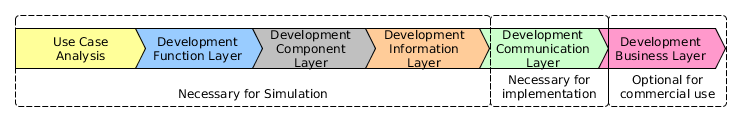
\includegraphics[width=14cm]{SGAM_mapping_steps}
		\caption{Prozess für Einordnung des Use Case im SGAM}
		\label{Abb:SGAM_mapping_steps}
	\end{figure} 
			
	Die meisten Bezahlsysteme der öffentlichen Ladesäulen konnten Ende 2017 mit öffentlichen Exploits gehackt werden, sodass beispielsweise Rechnungen zu Lasten voriger Ladepunktnutzer*innen und die Entwendung sensibler Daten nicht auszuschließen sind. \cite{CCC}  \cite{evsim}  \\ 	
	
	\section{Use Case Analysis}
		\label{Kap:Konzept_usecase}
			Der Anwendungsfall wird in Tabelle \ref{Tab:usecase} beschrieben und in Abbildung \ref{Abb:EMS} schematisch dargestellt. Die Abbildung fasst die Ladeinfrastruktur zu der CPS-unit \glqq Ladepunkte inkl. Laderegler\grqq zusammen und zeigt vereinfacht die Energie- und Datenflüsse. Zum Beispiel kommunizieren Ladepunktnutzer*innen mit dem EMS und dieses steuert die Energieflüsse. \\
            
            Das EMS kann sowohl in einer hierarchischen Struktur zentral gesteuert werden oder dezentral mit CPS-units, welche in einem Smart Grid miteinander kommunizieren und sich eigenintelligent selbst steuern. Eine dezentrale unhierarchische Kommunikationsstruktur ist deutlich komplizierter, daher wird für die Simulation der zentrale Ansatz gewählt. \\
            
		\begin{table}[h]
			\begin{tabularx}{\linewidth}{|c|X|}
				\hline 
				Name  		& Betrieb eines teilautarken Nanogrids mit Ladeinfrastruktur\\
				\hline 
				Aufgabenbereich 	& Überwachung und Regelung der Energieverteilung in\\
				(Scope) 			& teilautarkem Nanogrid mit konfigurierbarer Ladeinfrastruktur für E-Fahrzeuge durch zentrales EMS\\ 
				\hline 
				Ziel (Objective) 	& Überwachung und Regelung der Energieflüsse eines Nanogrids \\ 
				\hline
			\end{tabularx} 
			\caption{Name, Aufgabenbereich und Ziel des Anwendungsfall}
			\label{Tab:usecase}
		\end{table}
	
		\begin{figure}[h]
			\centering
			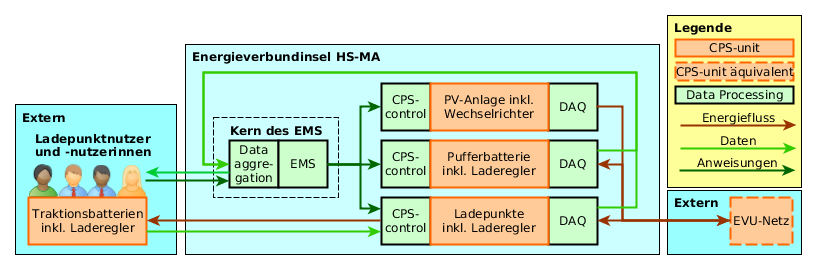
\includegraphics[width=14cm]{EMS}
			\caption{Schematische Darstellung der Energie- und Datenflüsse der Energieverbundinsel}
			\label{Abb:EMS}
		\end{figure}
			
		Anhand des Aufgabenbereichs wird eine Use Case Analysis durchgeführt. Alle Funktionalitäten und Akteur*innen  werden den SGAM-Zonen zugeordnet und in Abbildung \ref{Abb:usecaseanalysis} dargestellt. Eine Erklärung der Funktionalitäten ist in Tabelle \ref{Tab:usecase_zones} gelistet, die der Akteur*innen im Folgenden:\\
		
		\begin{itemize}
			\item Die CPS-units (EV, Ladepunktregler, PV-Anlage und Pufferbatterie) tauschen Energie im Nanogrid aus, werden überwacht und manche können gesteuert werden.
			\item Das Netz (Grid) tauscht mit dem Nanogrid Energie aus, kann jedoch nicht direkt gesteuert werden. 
			\item Benutzer*innen (User) konfigurieren den Ladevorgang, erhalten Daten und könnten optional Bezahlen.
			\item Das Bezahlungssystem (Payment System) für die Bestimmung der Nutzungskosten und Abwicklung der Zahlung ist optional.
			\item Das EMS (EMS) sammelt Daten, zeigt sie an, regelt die Energieflüsse durch Steuerung der CPS-units und macht die Energieflussregelung abhängig von User Konfigurationen
		\end{itemize}  

		\begin{figure}
			\centering
			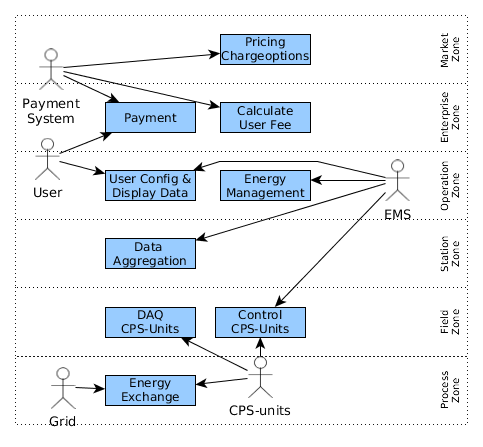
\includegraphics[width=0.6\textwidth]{usecaseanalysis}
			\caption{Usecase analysis der Energieverbundinsel mit teilautarker Ladeinfrastruktur}
			\label{Abb:usecaseanalysis}
		\end{figure} 
	

		\begin{table}
			\begin{tabularx}{\linewidth}{|c|X|}
				\hline 
				Zone & Beschreibung   \\ 
				\hline 
				Process 	& Austausch von Energie zwischen einzelnen CPS-units über Leitungen und Netzknoten \\ 
				\hline 
				Field 		& Messung und Steuerung übertragener Energie einzelner CPS-units \\
				\hline
				Station 	& Konzentration von Messdaten der einzelnen CPS-units \\
				\hline
				Operation 	& Konfiguration des Ladevorgangs und Regelung des Energymanagement aller CPS-units für den konfigurierten Ladevorgang \\
				\hline
				Enterprise 	& Kalkulation von Gebühren und Transaktionsverfahren für Bezahlungen \\
				\hline
				Market 		& Preisbilanzierung verschiedener Ladeoptionen \\
				\hline 
			\end{tabularx} 
			\caption{Beschreibung aller Funktionalitäten des Use Case mit Zuordnung der SGAM Zonen}
			\label{Tab:usecase_zones}
		\end{table}	
				
	\section{Funktionsebene des Konzeptes}
		\label{Kap:Konzept_func}
		Aus den bestimmten Funktionalitäten lassen sich die Funktionsebene ableiten und die funktionalen Abhängigkeiten bestimmen wie in Abbildung \ref{Abb:SGAM_map_func} gezeigt.\\
		
		Der Energieaustausch (Energy Exchange) von CPS-units wird gemessen (DAQ) und gesteuert (Control). Die aufgenommenen Messdaten einzelner CPS-units werden zentral gesammelt (Data Aggregation). Das Energiemanagement regelt Energieflüsse durch Steuerung der CPS-units und braucht dafür die konzentrierten Messdaten und User Konfigurationen (User Config).\\

		\begin{figure}[h]
			\centering
			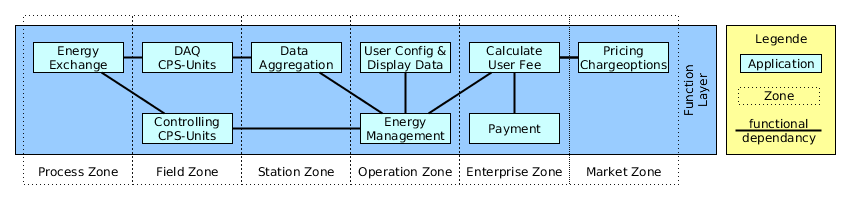
\includegraphics[width=14cm]{usecaseanalysis_func}
			\caption{Einordnung des Use Case in SGAM Zonen auf der Funktions-Ebene}
			\label{Abb:SGAM_map_func}
		\end{figure} 
	
		\subsection{Mögliche Konfiguration des Ladevorgangs} % Function Layer
			\label{Kap:Lademodelle}
			\subsubsection{Grundmodelle}
				In diesem Kapitel werden verschiedene Lademodelle für den Ablauf von Ladevorgängen für EV definiert. Diese können durch intelligente Regelung eines Energie- bzw. \ac{BMS} z.B. hinsichtlich minimaler Ladeverluste, Strompreisschwankungen, Netzstabilität oder \ac{SoH} optimiert werden. Dafür wurden einige Grundfunktionen in Tabelle \ref{Tab:Lademodelle} zusammengefasst und im Folgenden erklärt.\\
				
				\textbf{Kontinuierliche Ladung} ist eine Möglichkeit mit minimalen Ladeströmen, somit auch minimalen Ladestromverlusten, welche proportional zur Stromstärke im Quadrat auftreten. Kontinuierliche Ladungen führen zu einer gleichmäßig zeitlich verteilten, prognostizierbaren Last und beugen starken Leistungsgradienten vor.\\
			
				\textbf{Flexible Ladungen} müssen an bestimmte Vorgaben gekoppelt sein. Dieses Lademodell macht neben der vorraussichtlichen Anschlussdauer von weiteren Input-Parametern wie z.B. dynamischen Strompreisen oder Messwerten der Netzspannung bzw. -frequenz Gebrauch, welche in der Tabelle zusammengefasst als Ladekriterium benannt werden.\\ 
				
				\textbf{Sp"atladungen} können unter Umständen die Lebenszeit von Fahrzeugbatterien gegenüber einer kontinuierlichen Ladung erhöhen. LiFePO$_4$-Zellen, die z.B. oft in Notebookakkus oder E-Fahrzeugen verbaut werden, altern bei hohen Temperaturen und hohem SoC schneller. \cite[S.26]{FfE_Lademodelle_EAutos} Zu berücksichtigen ist dabei, dass Ladeströme sich ebenfalls auf den SoH auswirken. Vergleichsweise hohe Ströme werden durch höheren Verschleiß den SoH stärker beeinträchtigen, zu einer stärkeren Erwärmung und höheren Verlustleistungen führen.\\

				Je nach implementierter Hardware im Fahrzeug und verwendeter Ladesäulentechnik ist es theoretisch auch möglich zurück ins Netz zu speisen. Dieses Konzept wird \ac{V2G}, vom Fahrzeug ins Netz, genannt.\\
	
			\subsubsection{Beispiele kombinierter Modelle}
				Die Grundmodelle für Ladevorgänge lassen sich auch sequenziell zu komplexeren Lademodellen kombinieren. Im folgenden werden zwei einfache Beispiele mit Anwendungsfällen erläutert.\\
		
				\textbf{Kontinuierliche Ladung} und \textbf{Spätladung} lassen sich kombinieren zu einer später einsetzenden kontinuierlichen Ladung mit einer Ladeleistung zwischen der minimal für den Ladezeitraum nötigen und der maximal möglichen. Je genauer, die Auswirkungen auf den SoH der Batterie bestimmbar sind, desto genauer ließe sich der Ladealgorithmus einstellen, um den durch höhere Ladeströme bedingt größere Verschleiß zu berücksichtigen.\\
				
				\textbf{Sofortladung} und \textbf{flexible Ladung} lassen sich kombinieren. Im ersten Teil wird mit maximaler Leistung bis zu einem eingestellten SoC geladen und anschließend beginnt eine $flexible Ladung$ in welcher der vorher eingestellte SoC nicht unterschritten wird.  
		
				\begin{table}[h]
					\centering
					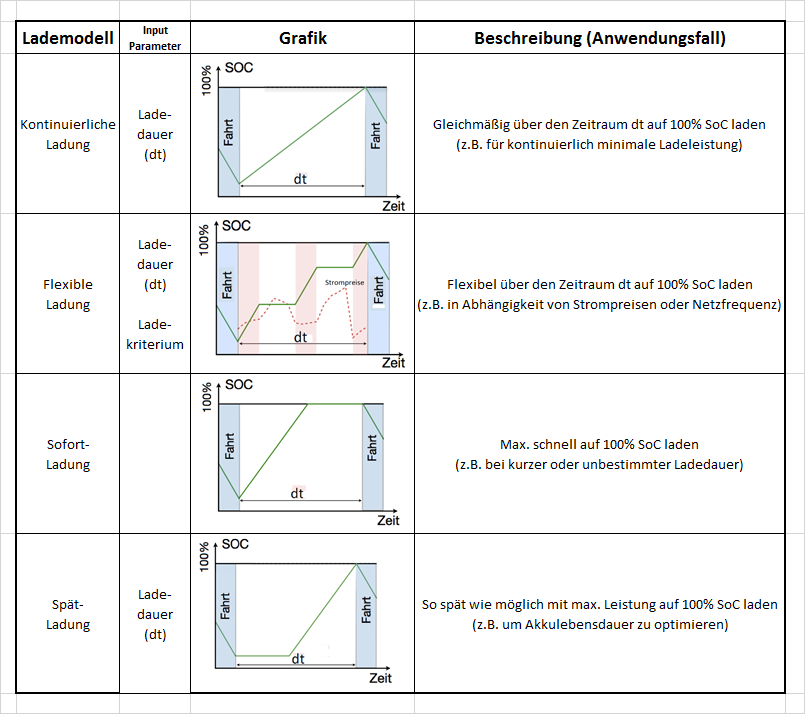
\includegraphics[width=16cm]{Lademodelle}
					\caption{Übersicht von Lademodellen nach \cite[modifizierte Grafiken]{FfE_Lademodelle_EAutos}}
					\label{Tab:Lademodelle}
				\end{table}

		\subsection{Konzept Energiemanagement}
		\label{Kap:DSM}
			Der Regelalgorithmus für das Energiemanagement eines EMS kann beliebig komplex gestaltet und hinsichtlich verschiedenster Aspekte optimiert werden. In diesem Kapitel wird ein einfacher Entwurf für die Laststeuerung \ac{DSM} mit einem Lademodus für die Pufferbatterie und drei konfigurierbaren Modi für die Ladepunkte gestaltet. \\

			Der logische Ablaufplan einer Simulation über T Zeitintervalle wird in Abbildung \ref{Abb:pap_dsm} gezeigt. Die For-Schleife entspricht einem Regelkreis mit der Regelgröße $P_{DSM}$, der Führungsgröße $0$ und der Stellgröße $P$, wobei in jeder Iteration die Planleistung von CPS-units der selben Priorität angepasst und damit $P_{DCM}$ abgeregelt wird.

			\begin{figure}[h] 
				\centering
				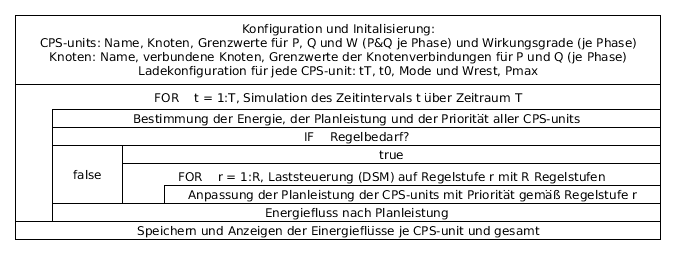
\includegraphics[width=\linewidth]{pap_dsm}
				\caption{Beispiel Ablaufplan für Energiemanagement mit mehreren Regelstufen}
				\label{Abb:pap_dsm}
			\end{figure}	
			
		\paragraph{Konfiguration} 
			% Ziel und Inputparameter
			User sollen die Lademodi $Mode$  Sofortladung (SofoL), Kontinuierliche Ladung (KontL) und Flexible Ladung (FlexL) einstellen und mit den Eingangsvariablen Anschlussdauer an Ladepunkt $dt$, zu ladende netto Batteriekapazität $W_{rest}$ und max. Ladeleistung $P_{max}$  konfigurieren können. \\  

		\paragraph{Bestimmung der Nennleistungen} %  P, Pn und \sum(Pn)	
			Die Planleistung $P_m$ einer CPS-unit $m$ wird zu Beginn eines Regelzyklus mit der zugehörigen Nennleistung $P_{m,n}$ gleichgesetzt $P_m = P_m,n~$. Diese wird abhgängig vom Lademodus bestimmt, bei Sofortladung (SofoL) mit der maximal möglichen Ladeleistung $P_{m,max}(SoC)$ und bei kontinuierlicher und flexibler Ladung (KontL und FlexL), so, dass der Energiebedarf $W_{m,rest}$ über den geplanten Anschlusszeitraum $dt_m$ durch eine kontinuierlich gehaltene Ladeleistung gedeckt wird. Die Nennleistung der Pufferbatterie $P_{m,n}(PB)$ entspricht der Summe aus der negativen PV-Ertragsleistung $P_{PV}$ und der Summe der Ladeleistungen von $M$ Ladepunkten. Alle Leistungswerte sind auf das Netz bezogen und entsprechen somit den Brutto-Ladeleistungen und Netto-Einspeiseleistungen. \\
			
			Für die Nennleistung innerhalb der Grenzwerte der verwendeten Ladepunkte gilt: \\
			$P_{m,n}(SofoL) = P_{m,max}(SoC)$  \\
            und ~ $P_{m,n}(KontL) = P_{m,n}(FlexL) = W_{m,rest}/dt_m$ \\
            und ~ $P_{m,n}(PB) = \sum_{m=1}^{M}(P_{m,n}) + P_{PV} $ 
			
			
			
		\paragraph{Bestimmung des Regelbedarfs}
			Ein Bedarf für die Regelleistung $P_{DSM}$ besteht, wenn die summierte Planleistung $P_{sum} = \sum_{m=1}^{M} P_m$ aller $M$ CPS-units mindestens in einer Phase an einem Knoten (Nanogrid) außerhalb der netzspezifischen Grenzwerte $P_{min,grid} ~\text{und}~ P_{max,grid}$ für die Übertragung zwischen Knoten der CPS-units und dem Netzknoten (Grid) liegt. Zu beachten ist, dass die PV-Anlage nicht am Netzknoten der Ladeinsel liegt und beim Energiemanagement nicht berücksichtigt wird. Im Verbraucherpfeilsystem gilt für $P_{DSM}$: 
					
		\begin{equation}
			\begin{split}
				P_{DSM} = P_{max}  - (P_{sum}) = P_{sum} > P_{max,grid} ~\text{bei geplanter Überlast}\\
				\text{und}~ P_{DSM} = 0 ~\text{für}~ P_{min,grid} < P_{sum} < P_{max,grid} ~\text{bei Betrieb in Normalbereich}\\	
				\text{oder}~ P_{DSM} =  P_{min}  - (P_{sum}) ~\text{für}~ P_{sum} < P_{min,grid} ~\text{bei geplanter Überversorgung}\\
			\end{split}  
		\end{equation}

		
			Im Nanogrid der Energieverbundinsel kann es aufgrund fehlender Energieerzeuger nur zu einem Regelbedarf an Erzeugungsleistung beziehungsweise Verbrauchsdrosselung kommen ($P_{sum}>P_{max,grid}$). Im Folgenden gilt daher pauschal $ P_{DSM} >= 0 $.
			

			
			
		\paragraph{Laststeuerung}
		% Allgemein
			Um den Regelbedarf $P_{DSM}$ an Regelleistung bereit zu stellen, können die Pufferbatterie mit $P_{max,PB}$ entladen und die genutzten $L$ Ladepunkte um die zugehörige Ladeleistungen $\sum P_{l} ~\text{mit}~ l=\big[1, ..., L\big]$ gedrosselt werden. Die neue Planleistung $P_{neu}$ kann mit einem Korrektursummanden $C$ oder einem Korrekturfaktor $k$ oder absolut mit $X$ beschrieben werden. \\ \\
			$P_{neu} = P + C \quad \text{mit} \quad P_{min} < P_{neu} < P_{max}$ \\   				
			
			In jeder Regelstufe teilen $L$ von $M$ CPS-units der zugehörigen Priorität den größtmöglichen Teil des neuen Regelbedarfs $P_{DSM,neu}$ unter sich auf. Dies geschieht gleichmäßig, bezogen auf die jeweils potientiell bereitstellbare Regelleistung. Für den Korrektursummand $C$ und -faktor $k$ gilt demnach: \\

			$P_{pot} = P - P_{min} \quad \text{für} \quad \sum_{1:l}^{L} P_{l,pot} > P_{DSM} >= 0$\\
            $\text{bzw.} \quad P_{pot} = P - P_{max} \quad \text{für} \quad P_{DSM} < 0 $ \\
			$C = P_{DSM} \frac{P_{pot}}{\sum_{1:l}^{L} P_{l,pot}}$ \\	
			
			Die Priorisierung von 1 bis 3 für CPS-units mit dem entsprechenden Lademodus wird in der folgenden Reihenfolge bestimmt: \\
			$ \text{prio} \big[1:3\big] \quad = \quad \big[\text{PB \quad FlexL \quad KontL oder SofoL}\big]$\\
							
			Der Algorithmus kann beliebig verändert und um Eingangsparametern erweitert werden wie z.b. mit $W$, $W_{max}$, $dt$ der Batterien (EVs und PB), PV-Leistung $P_{PV}$ und Wetter-/Lastprognosen.
			


% NOTE: HINWEISE ANFANG
% Hinweis: SoC Bestimmung		
	% Der anfängliche $SoC$ muss entweder durch die Kommunikation zwischen EV und Ladepunkt oder eine Usereingabe gegeben sein.\\ % NOTE: Ev. weg? Kommunikations-Ebene

% Hinweis Vorzeichensetzung
	% Das Verbraucherpfeilsystem wird auf alle CPS-units angewandt, sodass Leistungen mit positivem Vorzeichen einer Netzeinspeisung und negativem einem Netzbezug entsprechen. \\
% NOTE: HINWEISE ENDE
			
					
			
	\section{Informations- und Komponenten-Ebene des Konzeptes}
	\label{Kap:Konzept_comp}
		In Abbildung \ref{Abb:SGAM_map_all_total} wurde die SGAM-Visualisierung um die Informations- und Kom-\\ponenten-Ebene erweitert. Gezeigt wird die interebenen Kommunikation zwischen den Ebenen sowie die innerebenen, funktionalen Abhängigkeiten der User, Anwendungen, Info Objekten, Geräten und Netz. \\
		
		Die CPS-units (Ladepunkte, PB, PV-Anlage) tauschen Energie mit dem Netz aus und werden von Smart Metern überwacht und Controllern gesteuert. Die Messdaten werden von einem Data Collector gesammelt. Dieser kann mit dem EMS-Controller verbunden sein oder mit diesem in einem Gerät umgesetzt sein. Der EMS-Controller koordiniert mit den User Konfigurationen vom User Interface die CPS-Controller, um die Energie im Nanogrid zu managen. \\
		
		Im Folgenden werden die für die Berechnung der Energieflüsse verwendeten Datenmodelle beschrieben. Die Komponenten-Ebene wird nur skizziert, um den Prozess auf physikalischer Ebene besser zu veranschaulichen und für zukünftige Arbeiten eine Übersicht zu schaffen. Eine detaillierte Auflistung der Komponenten auf Prozess-Ebene wurde bereits erarbeitet. \cite{BA_Chris_Ong_2017}
	
%			\begin{figure}[h] % NOTE REF
%				\centering
%				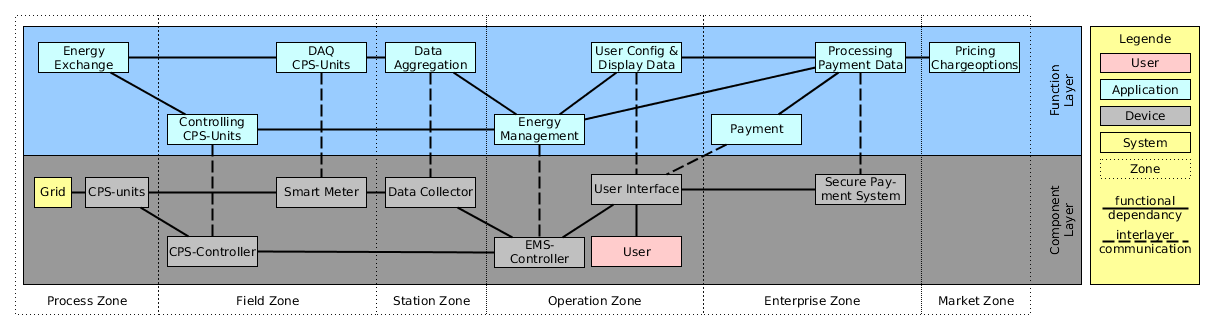
\includegraphics[width=14cm]{usecaseanalysis_func_comp}
%				\caption{Einordnung des Use Case in SGAM Ebenen Function und Component über alle Zonen}
%				\label{Abb:SGAM_map_func_comp}
%			\end{figure} 


			\begin{figure}[h] % NOTE REF
				\centering
				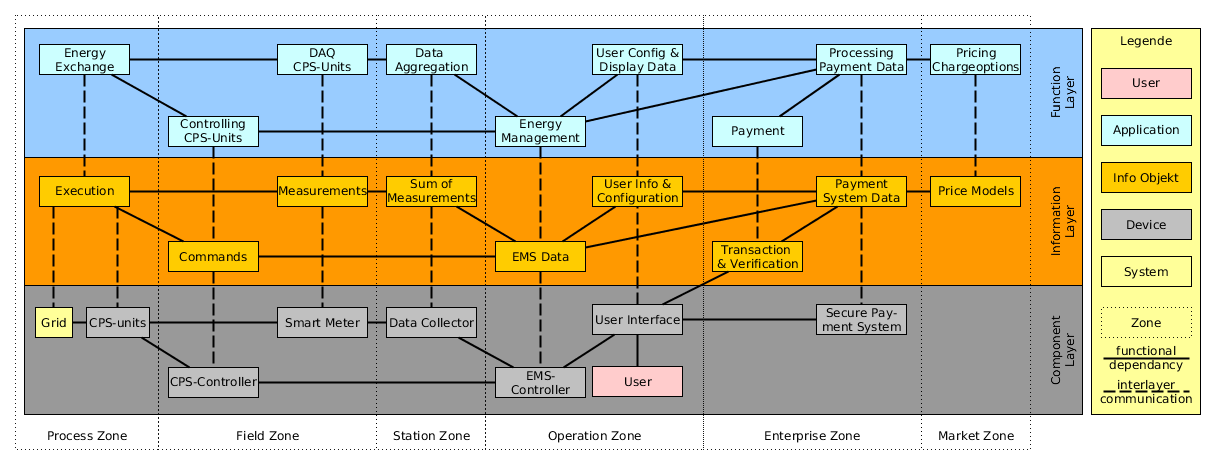
\includegraphics[width=14cm]{usecaseanalysis_all_total}
				\caption{Einordnung des Use Case in SGAM Ebenen Function, Information und Component über alle Zonen}
				\label{Abb:SGAM_map_all_total}
			\end{figure} 
					
		\subsection{Datenmodelle der Info-Objekte in Matlab Syntax}
			Um die in Kapitel \ref{Kap:Konzept_func} beschriebenen Funktionalitäten zu gewährleisten, werden die benötigten Informationen verschiedenen Info-Objekten zugeordnet. In diesem Kapitel werden hierfür die in der Simulation verwendeten Datenmodelle des Info-Objektes $EMS Data$ und $User Konfiguration$ erstellt. Für die $EMS Data$ wird die Datenstruktur für CPS-units (cps) und für Netzknoten (nodes) in Matlab Syntax definiert und ebenso die $User Konfiguration$ für Einstellungsparameter der Ladevorgänge (cpsuse) definiert. \\

			\paragraph{Prototyp Strukturdefinition der CPS-units (cps)}~ \\
			Die Attribute jeder CPS-unit werden, wie in Listing \ref{Code:prototype_cps} gezeigt, mit einem Array aus Zellen mit jeweils einer Varable des Datentyps $struct$ beschrieben. Jede Variable des Typs $struct$ ist wiederum ein Array mit Variablen (optional) unterschiedlicher Datentypen, die jeweils einem Feld (field) zugewiesen werden. Die Attribute einer $struct$ Variable können gelesen und beschrieben werden mit der Schreibweise <name struct variable>.<name struct field>, z.B. $cps.id~ = 'PV'$. Der Ansatz mithilfe von $struct$ Variablen bietet die Möglichkeit, im Nachhinein weitere Felder hinzuzufügen, ohne, dass die Funktionalität des bestehenden Codes beeinträchtigt wird. Denkbar sind beispielsweise die Temperatur, der SoH, oder dass bisher statische Eigenschaften wie der Wirkungsgrad dynamisch beschrieben werden. \\
            

            
	          \begin{lstlisting}[language=Matlab,caption=Funktion zur Strukturdefinition der CPS-units, label=Code:prototype_cps]
  % CPS STRUCTURE (consumer-producer-storage)
  % static fields
  cpsstruct.id   = '';            % string, name of CPS-units
  cpsstruct.node = '';            % string, name of connected node
  cpsstruct.pmin = [0,0,0];       % numeric (3x1), min. active power on phases [kW]
  cpsstruct.pmax = [0,0,0];       % numeric (3x1), max. active power on phases [kW]
  cpsstruct.qmin = [0,0,0];       % numeric (3x1), min. reactive power on phases [kvar]
  cpsstruct.qmax = [0,0,0];       % numeric (3x1), max. raective power on phases [kvar]
  cpsstruct.wmax = 0;             % numeric, netto battery capacity [kWh]
  cpsstruct.eta  = [0,0,0];       % numeric (3x1), power efficiencies eta(1), eta(2) 
  % and rate of energy degradation per hour eta(3) 
  % .w(t+1) = .eta(3)*.w(t) + .eta(1)*.p(t) with .p(t) > 0
  % .w(t+1) = .eta(3)*.w(t) + .eta(2)*.p(t) with .p(t) < 0 
  % efficiencies eta(1) for positive power, eta(2) for negative power
  % eta(3) as relative energydegradation per timeinterval
  
  % dynamic fields
  cpsstruct.prio = 0;           % scalar, priority
  cpsstruct.p = [0,0,0];        % numeric (3x1), sum of active power [kW]
                                % on each phase of every connected CPS-unit
  cpsstruct.q = [0,0,0];        % numeric (3x1), sum of reactive power [kW]
                                % on each phase of every connected CPS-unit
  cpsstruct.w = 0;              % scalar, netto capacity [kWh]
    	      \end{lstlisting}
			
			\paragraph{Prototyp Strukturdefinition der Ladevorgangskonfiguration der CPS-units (cpsuse) und der Netzknoten (node)} ~\\
             Für den Usecase der jeweiligen CPS-unit wie beispielsweise einstellbarer Ladesequenzen und für die Netzknoten (nodes) im Nanogrid wird jeweils der gleiche Ansatz mit Variable des Typs $struct$ gewählt. Der zugehörige Code wird in den Listings \ref{Code:prototype_cpsuse} und \ref{Code:prototype_node} gezeigt. \\
            

          \begin{lstlisting}[language=Matlab,caption=Funktion zur Strukturdefinition der CPS-Unit zugehörigen Usecases, label=Code:prototype_cpsuse]
  % CPSUSE STRUCTURE
  cpsusestruct.info = '';     % string, additional information
  cpsusestruct.id   = '';     % string, name of CPS-units
  cpsusestruct.mode = '';     % string, type of usecase e.g. 'KontL' for continuously charging
  cpsusestruct.w0   = 0;      % scalar, initial energy at start time t0
  cpsusestruct.wmax = 0;      % scalar, maximal energy (SoC 100 %)
  cpsusestruct.t0   = 0;      % scalar, start time, 
  cpsusestruct.tT   = 0;      % scalar, end time
          \end{lstlisting}			

          \begin{lstlisting}[language=Matlab,caption=Funktion zur Strukturdefinition der Netzknoten, label=Code:prototype_node]
  % NODE STRUCTURE
  % static fields
  nodestruct.id = {''};               % string, name of node
  nodestruct.link = {''};             % string array, name(s) of connected node(s)
  nodestruct.pmax = {[0,0,0]};        % numeric (3x1), max. sum of active power [kW]
                                      % on each phase of every connected CPS-unit
  nodestruct.qmax = {[0,0,0]};        % numeric (3x1), max. sum of raective power [kvar] 
                                      % on each phase of every connected CPS-unit

  % dynamic fields
  nodestruct.p = {[0,0,0]};           % numeric (3x1), sum of active power [kW]
                                      % on each phase of every connected CPS-unit
  nodestruct.q = {[0,0,0]};           % numeric (3x1), sum of reactive power [kW]
                                      % on each phase of every connected CPS-unit
          \end{lstlisting}
			
            \paragraph{Konfigurationsdaten in CSV-Format} ~\\
            Für eine einfache Initialisierung mit Wertzuweisungen der $struct$ Variablen, werden Matlab-Skripte in Form geschrieben, welche die entsprechenden Eigenschaften in tabellarischer Form aus CSV-Dateien auslesen und einem Array aus $struct$ Variablen zuweisen. Der Name der dritten CPS-unit wird beispielsweise aus dem Zellen-Array $cps$ mit $cps{3}.id$ abgerufen. Die CSV-Dateien mit Konfigurationsdaten sind in tabellarischer Form im Anhang in den Tabellen \ref{Tab:cfg_cps}, \ref{Tab:cfg_node}, \ref{Tab:cfg_cpsuse_wc}, \ref{Tab:cfg_cpsuse_nc} und \ref{Tab:cfg_cpsuse_bc} für alle drei Szenarien dargestellt. \\
			
%		\subsection{Process} % Component Layer	
%		\label{Kap:Process}
%		Ladeschränke:
%			https://www.lad-e.com/ladeschrank-f%C3%BCr-e-bikes/
%			https://rotstahl.de/produkt/akku-ladeschrank-e-bike-pedelec-cart/
%		
%			\subsubsection{Ladetechnik}
%			\label{Kap:Ladetechnik}
%				Die Ladetechnik der Pufferbatterie sollte die Möglichkeit bieten, die Batterie mit definierter Leistung über eine Stromregelung zu laden, wobei das Leistungslimit der Leistungselektronik im Laderegler die maximale Leistung der Batterie nicht übersteigen sollte. \\
%				
%				Für eine Netzintegration von Elektrofahrzeugen mit dem Ziel der Nutzung der Traktionsbatterien als Energiespeicher in einem Smart Grid (Vehicle to Grid, V2G), ist eine Ladetechnik notwendig, die bidirektionales Laden und damit Netzeinspeisungen ermöglicht.\\
%				
%				Einige E-Autos verfügen bereits über die Option einer Netzeinspeisung, darunter zum Beispiel 
%				der Opel Elektro-Meriva, 
%				der Nissan Leaf (CHAdeMO), e-NV200
%				der Mitsubishi EV (aka i-MiEV) ab Baujahr 4/2014 (CHAdeMO), 
%				der Mitsubishi Outlander Plug-In-Hybrid (PHEV)(CHAdeMO),
%				Theoretisch CCS-Anschluss, z.B. bei VW oder BMW\\
%				
%				
%			\subsubsection{Messtechnik}
%				Für die Leistungserfassung müssen für jede Phase Wirk- und Blindleistung gemessen werden. Für die Bestimmung des SoC der Traktions- und der Pufferbatterie ist die Messung der Batteriespannung, -ströme und -temperatur nötig. 
%				
%				Die Messtechnik muss für Spannungslevel in der Größenordnung von XYZ bis XYZ V und Ströme bis zu XYZ A ausgelegt werden. 
%			
%			\subsubsection{Steuertechnik}
%
%			
%			\subsection{Kommunikationstechnologie}
%			
%	
%						
%	\section{Softwareanforderungen} % Communication and Information Layer
%	\label{Kap:EMS_Anforderung_SW}
%
%		Zusammenfassung von CPS-units zu selbstregulierenden Microgrids	
%		Skalierbar für Anschluss zusätzlicher CPS-units/Microgrids		
%		Steuerung im Kleinen wie im Großen	
%		Idealerweise sowohl für Energiemanagement von realen als auch simulierten CPS-units
		

		
 % Externe Datei einbinden
\chapter{Energieflussberechnungen verschiedener Szenarien}
\label{Kap4}
	% Vorstellung des Kapitels und der Szenarien
	In diesem Kapitel wird die Simulation für die Energieflussberechnungen durchgeführt. Zu Beginn werden hierfür die notwendigen Randbedingungen in definiert. Es gibt eine Auswahl an Szenarien, welche die nach Voreinschätzung bestmöglichen, möglichst durchschnittlichen und die schlechtest möglichen Bedingungen abdeckt. Diese werden im folgenden mit \ac{BC}, \ac{NC} und \ac{WC} abgekürzt. In Abb. \ref{Abb:Szenarien} ist eine Übersicht der Szenarien mit den variierenden Parametern dargestellt. Nach Definition der Randbedingungen folgt eine kurze Beschreibung des entwickelten .m-Codes und die Simulationsergebnisse.
    
	% Erstellung der Erzeugungsprofile mit Code für Wetteranalyse
%		In den untersuchten Fällen variiert Erzeugungsprofil und das Lastverhalten wie in Kapitel \ref{Kap:Festlegung_Szenarien} bis \ref{Kap:Sim_cfg_con} definiert. \\
	
	% Erstellung der Ladeprofile mit Code für Simulation
	
	% Code für Simulation
	
	% Simulation und Auswertung
	
	
	\begin{figure}[h]
		\centering
		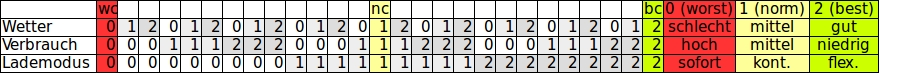
\includegraphics[width=\textwidth]{Szenarien.jpg}
		\caption{Übersicht der variablen Parameter innerhalb der ausgewählten, farblich markierten, Szenarien}
		\label{Abb:Szenarien}
	\end{figure}

\section{Festlegung der Randbedingungen}
	\label{Kap:Festlegung_Szenarien}
	Die szenarienübergreifenden Randbedingungen werden wie folgend definiert und sind abgesehen von der zeitlichen Auflösung tabellarisch in Kapitel \ref{Kap:Konfiguration} gelistet. Die zeitliche Auflösung der Simulation liegt bei 1h, die betrachtete Zeitspanne bei 24~h. Die Netztopologie sowie die Kenndaten der Ladepunkte und der Pufferbatterie entsprechen dem Konzept aus Kapitel \ref{Kap:Vorgaben}. Die Ladepunkte inklusive -regler und Batterie besitzen einen Wirkungsgrad von $\eta_{LP} = 85 \%$. Die maximale Übertragungsrate zwischen Knoten $n1$ mit allen Ladepunkten und der Pufferbatterie und Knoten $n2$ mit PV-Anlage und Netz liegt bei $P_{max,grid} = 50 kW$. Der Algorithmus zur Bestimmung der Nennleistungen für alle Ladepunkte und die Pufferbatterie und für DSM wird aus Kapitel \ref{Kap:DSM} übernommen und um die Wirkungsgrade ergänzt. 
    
    \subsection{Auswahl der Pufferbatterie}
    		Als Pufferbatterie wird aufgrund der in Kapitel \ref{Kap:Akkus} beschriebenen Vorteile ein Bleikristallakku ausgesucht. Es werden drei Akkus des Modells Lead Crystal 6-CNFJ-120 des Herstellers  $\text{Lead Crystal}^{\textsuperscript{\textregistered}} ~\text{Batteries}$ mit jeweils einem IUoU Automatikladegerät (12~V~/~50~A) des Herstellers Fraron für jede Phase ausgewählt. Die Datenblätter sind im Anhang als Abbildung \ref{Abb:datasheet_akku} und \ref{Abb:datasheet_laderegler} gelistet. \\
        
        Die Zellen haben eine Spannung von jeweils 12~V und eine Bruttokapazität von jeweils 100~Ah (1,2~kWh). Die maximal mögliche Ladeleistung je Zelle beträgt 0,6~kW. Die Kosten für Akkuzellen (je 391,90 Euro) und Laderegler (je 299,00 Euro) exklusive Versand liegen zusammen bei ca. 2070,00~Euro. Für die Simulation wird der DoD der Pufferbatterie auf 95~$\%$, der anfängliche SoC der Pufferbatterie auf $50~\%$ und der Lade- und Entladewirkungsgrad inklusive Ladereglerverlusten $\eta_{PB}$ auf $90~\%$ gesetzt.\\
        
        In Tabelle \ref{Tab:PB_Dim} wird anhand der Herstellerangabe der optimale DOD für die 3 oben genannten Akkus mit maximaler Brutto Speicherkapazität über die Lebenszeit berechnet. Zudem wird eine Abschätzung der Rentabilität des Akkus vorgenommen. \\ 
       
        \begin{table}[h]
          \centering
          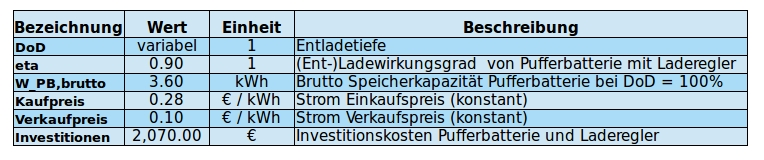
\includegraphics[width=\textwidth]{PB_Dim_stat} \\
          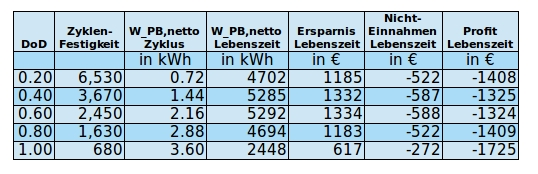
\includegraphics[width=\textwidth]{PB_Dim_dyn}         
          \caption{Bestimmung der optimalen Entladetiefe der Pufferbatterie und Abschätzung des erzielten Profits der Pufferbatterie über die Lebenszeit gerechnet anhand der Zyklenfestigkeit Z}
          \label{Tab:PB_Dim}        
        \end{table}    

		Die Ersparnis ergibt sich aus der Menge nicht eingekaufter Energie und die Nicht-Einnahmen anhand der nicht verkauften Energie über die Lebenszeit. Hierfür wird von einem Kalkulationszins von $0~\%$ und konstanten Strompreisen ausgegangen. Unter den getroffenen Annahmen amortisiert sich die Pufferbatterie nicht innerhalb der Lebenszeit. Bei einem DoD von 60~$\%$ würden sich die Akkus erst bei einem durchschnittlichen Stromkaufpreis von 55,8~$\frac{ct}{kWh}$ - ca. das doppelte heutiger Strompreise - unter sonst gleichen Bedingungen gerade so über die Lebenszeit amortisieren. \\
        
        Um das Betriebsverhalten einer Pufferbatterie in der Simulationsumgebung zu testen werden alle Szenarien trotz nicht wirtschaftlicher Betriebsweise der Pufferbatterie einmal mit den oben spezifizierten Kennwerten berechnet. \\
					
	\subsection{Erzeugungsprofile der PV-Module}
		\label{Kap:Sim_cfg_gen}
		Die Erzeugungsprofile werden anhand der Kenndaten in Tabelle \ref{Tab:PV_kenndaten} der installierten PV-Anlage und den in \ref{Kap:Sim_cfg_gen_data} ausgewählten Globalstrahlungsdaten erstellt, da von der Anlage keine geloggten Erzeugungsdaten über einen längeren Zeitraum zur Verfügung stehen. \\
	
		Der Wirkungsgrad der PV-Module wird modellhaft als konstant angenommen und nach Gleichung \ref{Eq:PV_eta} unter Einsetzen der Kenndaten aus Tabelle \ref{Tab:PV_kenndaten} ermittelt, wobei die Einheiten $W$ und $Wp$ sich herauskürzen. \\
		
			$ \eta_{PV} = (\frac{P_p}{A}) / G_{STC} = (\frac{20145 Wp}{76 \cdot 1,65 m^2}) / (1000 \frac{W}{m^2}) = 16,06 \% $ \\
			
		Die eine Hälfte der Module ist nach Bemessung des Konstruktionsplans in Abbildung \ref{Abb:datasheet_pv_4} unter Annahme einer maßstabsgetreuen Abbildung zu ca. $13,2 \degree$ nach Osten geneigt, während die andere Hälfte symetrisch dazu nach Westen geneigt ist. Zur Einfachheit wird von horizontal angebrachten PV-Modulen ausgegangen. \\
		
		Genauere Ergebnisse können erzielt werden, wenn unter Berücksichtigung der Geoposition, Ausrichtung, Neigungswinkel und Uhrzeit die senkrecht auf die Modulflächen eintreffende Globalstrahlung aus der senkrecht auf die Erdoberfläche eintreffende Globalstrahlung berechnet wird. Die Umrechung der Globalstrahlung von einer ebenen auf eine geneigte Fläche, wie in Kapitel \ref{Kap:G0g} beschrieben, ist noch nicht im Code implementiert. \\			

		\subsubsection{Globalstrahlungsdaten für Mannheim}	
			\label{Kap:Sim_cfg_gen_data}
			Der \ac{DWD} stellt von zahlreichen Wetterstationen Solarstrahlungsdaten (global und diffus), in einer Auflösung von bis zu 10 Minuten auf dem FTP-Server ihres Climate Data Center frei zur Verfügung.\cite{DWD} \\
			
%			Die verwendeten Daten stammen aus Mannheim von der Station mit der ID 05906 und wurden in einer Höhe von 96 m über dem Meeresspiegel am Standort 49.5090° geographischer Breite und 8.5541° geographischer Länge gemessen.\cite{DWD}
			
			Angesichts der Ungenauigkeit der Repräsentativität manuell erstellter Verbrauchs-profile wird eine zeitliche Auflösung von einer Stunde für die dem Erzeugungsprofil zugrunde liegenden Globalstrahlungsdaten als hinreichend genau betrachtet. Eine fest definierte Auflösung von einer Stunde verringert den Programmier- und Rechenaufwand gegenüber höheren oder dynamisch einstellbaren Auflösungen.  \\
						
%			StationsID:	ID 05906 (Mannheim)\\
%			Höhe über dem Meeresspiegel:	96 m\\
%			geographische Breite:	49.5090°\\
%			geographische Länge:		8.5541°\\
					
			Für die Auswahl geeigneter Tage wird mithilfe des in \ref{Kap:Sim_cfg_gen_code} beschriebenen .m-Codes ein Datensatz des DWD mit Tagessummen der Globalstrahlung für die Wetterstation in Mannheim mit der ID 05906 auf 96 m Höhe über dem Meeresspiegel, dem geographischen Breitengrad 49.5090° und geographischen Längengrad 8.5541° untersucht. \\

			Von den verfügbaren Wetterdaten im folgenden Zeitraum wahrer Ortszeit (WOZ) werden die neusten 21 Jahre untersucht: \\
			Zeitraum verfügbar:\quad 	von 01.01.1979 00:00 Uhr \quad bis 01.01.2012 00:00 Uhr \\
			Zeitraum untersucht:\quad 	von 01.01.1991 00:00 Uhr \quad bis 01.01.2012 00:00 Uhr \\

%			Die Datensätze haben laut DWD ein Qualitätsniveau von eins, was bedeutet, dass nur eine formale Prüfung beim Entschlüsseln und Laden der Daten durchgeführt wurde. Im zur Verfügung stehenden Zeitraum sind 78 der 12053 Tage mit inplausiblen Werten versehen.
            
			\subsubsection{.m-Code für Auswertung von Globalstrahlungsdaten}
			\label{Kap:Sim_cfg_gen_code}
            	Das Programm $weatheranalysis.m$ wertet die Globalstrahlungsdaten des DWD mit zeitlicher Auflösung von einer Stunde und einem Tag aus. In einem definierten Zeitintervall der zur Verfügung stehenden Daten sucht der Code den Tag mit der maximalen, minimalen und der geringsten Differenz zur durschnittlichen Globalstrahlung für die Szenarien \ac{WC}, \ac{NC}, \ac{BC} heraus. Zu jedem Tag werden unter Berücksichtigung der Peakleistung der PV-Anlage die Modulerträge ermittelt. Die Ertragsdaten beinhalten keine Wechselrichter- und keine Kabelverluste und werden in einer CSV-Datei mit Zeitstempel gespeichert. \\

Der vollständige Code der Datei $weatheranalysis.m$ wird in Kàpitel \ref{Kap:Code} gezeigt. Das funktionstüchtige Programm mit allen weiteren Dateien für Funktionsdefinitionen und Konfigurationsdaten sind über die beigelegte CD und über Github verfügbar. \cite{github_energyflowsim} Die Benutzer*innen-Anleitung ist einer README Datei beigefügt. \\

%			\lipsum
			\begin{figure}[h]
				\begin{minipage}{0.49\textwidth}
					\centering
					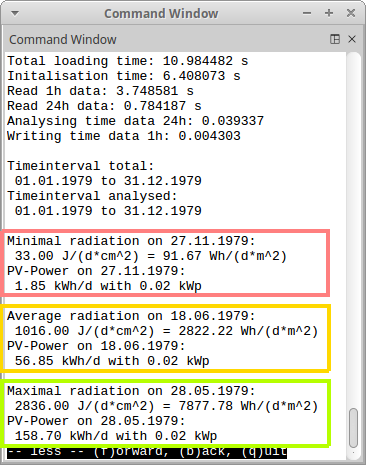
\includegraphics[width=\textwidth]{weather_res_test}
				\end{minipage}\hfill
				\begin{minipage}{0.49\textwidth}
					\centering
					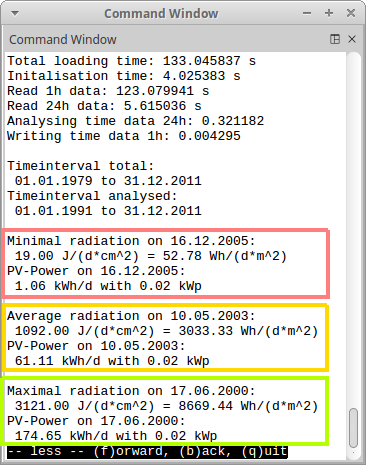
\includegraphics[width=\textwidth]{weather_res}
				\end{minipage}
				\caption{.m-Code Auswertung von Wetterdaten eines Datensatezs über 1 Jahr und über 32 Jahre \\ Farbkennung: Grün: BC, Gelb: NC, Rot: WC}
				\label{Abb:weather_res}
			\end{figure}
%			\lipsum[3]

			Getestet wurde der Code mit einem gekürzten Testdatensatz der einstündigen Wetterdaten im Zeitraum vom 01.01.1979 bis 31.12.1979. Um die Ergebnisse zu überprüfen, wurde der Testdatensatz mithilfe des Tabellenkalkulators Libre Office auf inplausible Datenreihen, minimal, maximal und dem Durchschnitt am nächsten kommende Globalstrahlungsdaten untersucht. Die Auswertung der Testdaten mittels Code in Abbildung \ref{Abb:weather_res} (rechts) und mittels Tabellenauswertung in Abbildung \ref{Abb:weather_verify} sind identisch. Inplausible Daten werden fehlerfrei heraus gefiltert und fließen nicht in die Mittelwertsberechnung oder die Minimasuche ein. \\
						
			\begin{figure}[h]
				\centering
				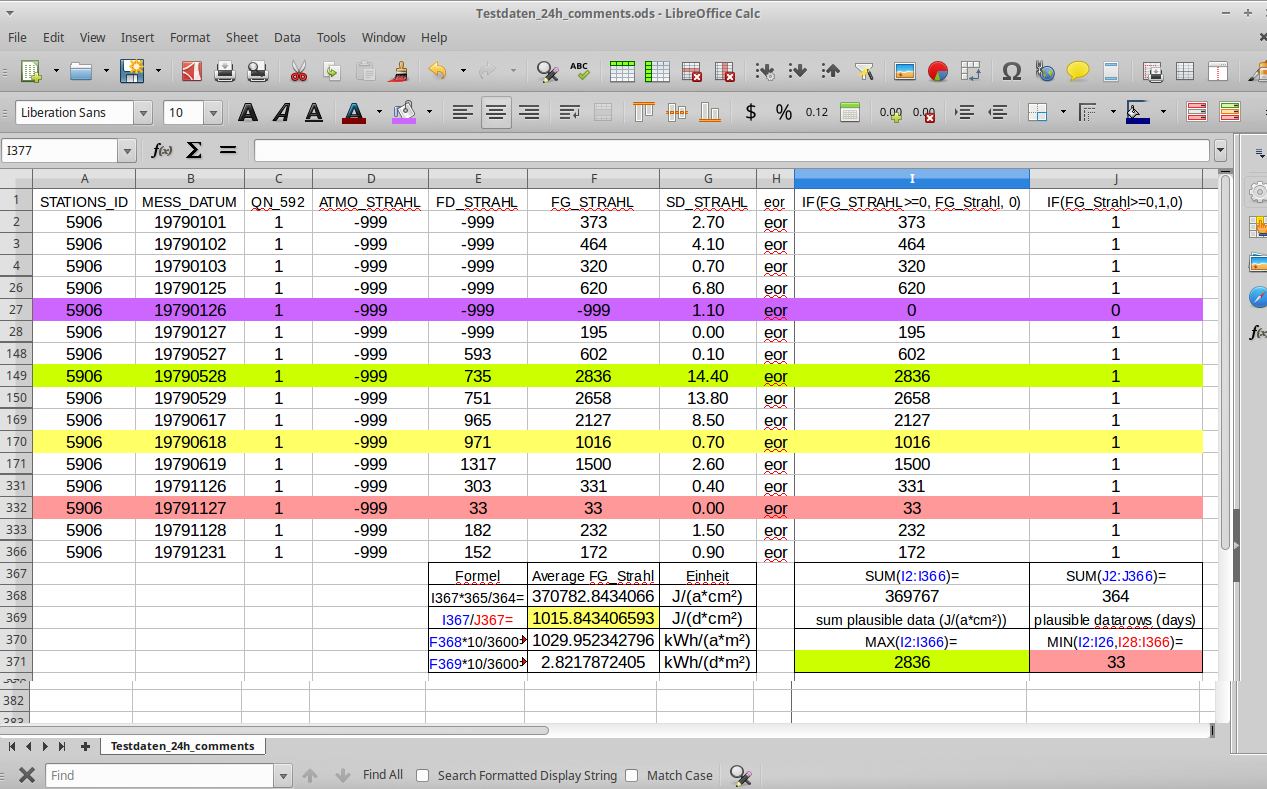
\includegraphics[width=14cm]{weather_verify}
				\caption{
					Überprüfung der Wetterdatenauswertung mit .m-Code in Tabellenkalkulator \\ 
					Farbkennung: Purpur: unplausible Messreihe, Grün: BC, Gelb: NC, Rot: WC \\ 
					ATMO\_STRAHL: Tagessumme der atmosphärischen Gegenstrahlung $\frac{J}{d*cm^2}$\\
					FD\_STRAHL: Tagessumme der diffusen solaren Strahlung $\frac{J}{d*cm^2}$\\
					FG\_STRAHL: Tagessumme der Globalstrahlung $\frac{J}{d*cm^2}$\\
					SD\_STRAHL: Tagessumme der Sonnenscheindauer in $h$\\
				}
				\label{Abb:weather_verify}
			\end{figure}
			
			Die durschnittlich ermittelten Globalstrahlungswerte von ca. 1000 und 1100 $\frac{J}{d*cm^2}$ entsprechen mit etwa $1014\frac{Wh}{a*m^2}$ und $1115\frac{Wh}{a*m^2}$ mit $1\frac{J}{d*cm^2} = \frac{365*100^2}{60^2}\frac{Wh}{a*m^2}$ den typischen Werten für Deutschland zwischen 900 und 1200 $\frac{kWh}{a*m^2}$. \cite{DWD} \\
            
            Die ermittelten Ertragsleistungen $PV-Power$ stellen die Ausgangsleistung der PV-Module dar. Abbildung \ref{Abb:PV_gen} zeigt die Ertragsleistung der PV-Anlage für alle drei Szenarien in Form von Ertragsprofilen mit einem Systemwirkungsgrad von 90\% für Wechselrichter- und Kabelverluste. 

					\begin{figure}[h] % NOTE: Derzeit noch Globalstrahlung in J/cm^2
						\centering
						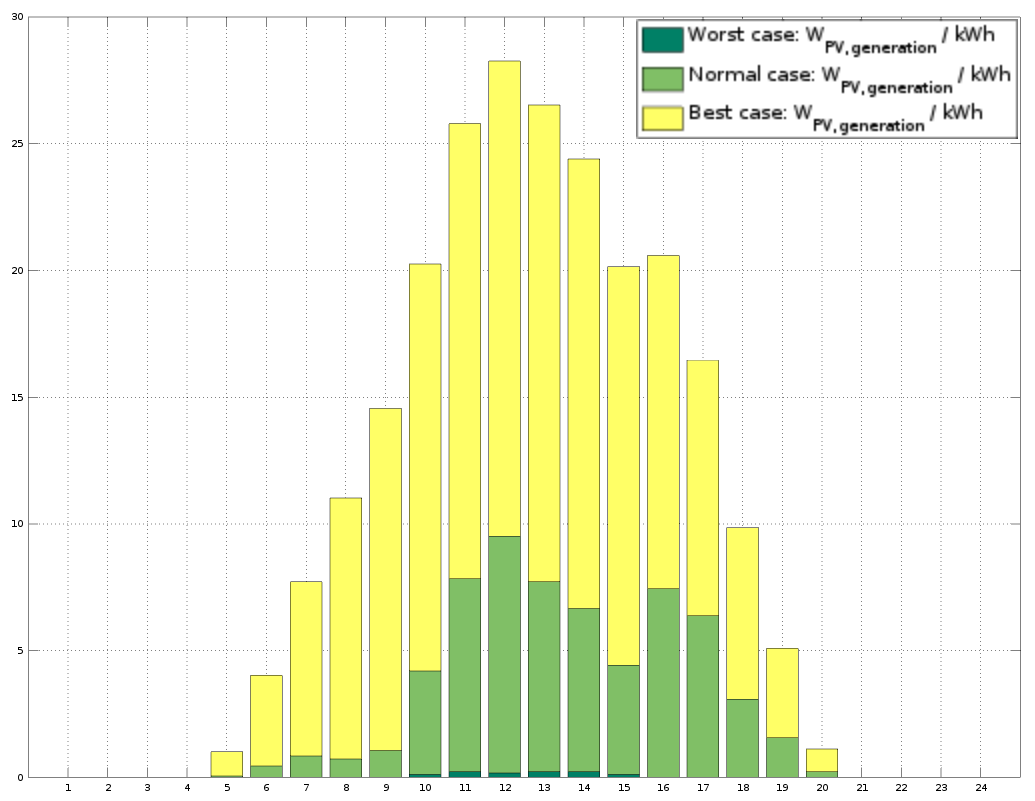
\includegraphics[width=14cm,height=7cm]{W_pv_gen_all}
						\caption{Netto Erzeugungsprofil der PV-Anlage im Worst, Normal und Best Case über 24~h}
						\label{Abb:PV_gen}
					\end{figure}
			
			% NOTE PV Power inplausible!
			
%			Daten: \\
%				Stundensumme der atmosphärischen Gegenstrahlung $\frac{J}{cm²}$\\
%				Stundensumme der diffusen solaren Strahlung $\frac{J}{cm²}$\\
%				Stundensumme der Globalstrahlung $\frac{J}{cm²}$\\
%				Stundensumme der Sonnenscheindauer $min$\\
%				Zenitwinkel der Sonne bei Intervallmitte $Grad$\\
%				Intervallende in WOZ $yyyymmddhh$\\
%				Intervallende in UTC $yyyymmddhh$\\
				

	
	\subsection{Lastprofile der E-Fahrzeuge}
	\label{Kap:Sim_cfg_con}
		Die Lastprofile werden durch das EMS abhängig von den vordefinierten Ladevorgängen, von der eingesetzten Pufferbatterie und von der zur Verfügung stehenden PV-Leistung berechnet. Die Ladevorgänge werden, wie in Kapitel \ref{Kap:DSM} beschrieben, mit den Parametern $t0$, $tT$, $Mode$, $W0$, $Wmax$ und $Pmax$ konfiguriert. Aufgrund der in Realität unterschiedlicher, stark fluktuierender Nutzung werden für die Bestimmung der Szenarien mehrere grobe Annahmen getroffen und ein am Wetter orientiertes Nutzungsverhalten mit Tag- und Nachtladungen modelliert. \\
        
		\begin{figure}[h]
			\centering
			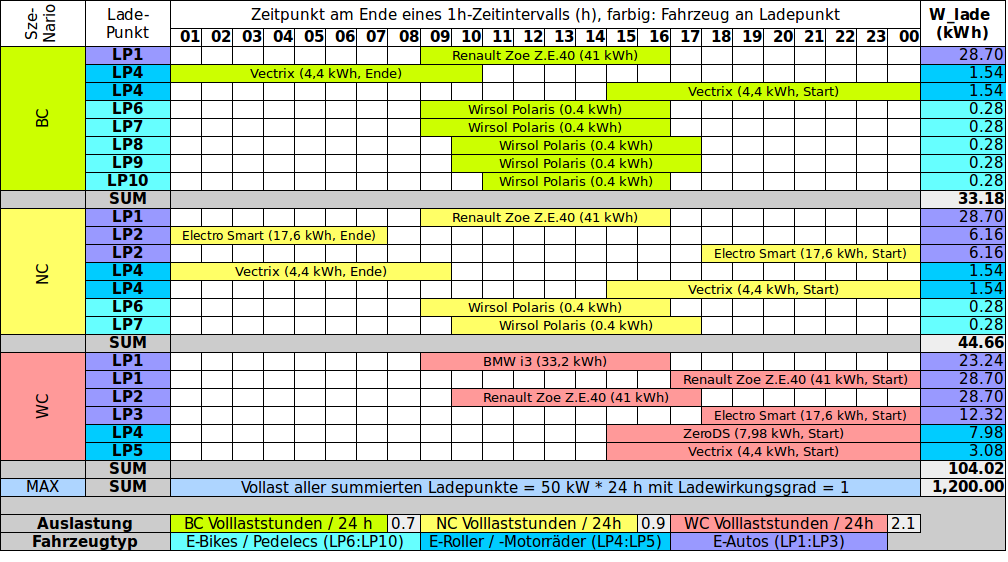
\includegraphics[width=14cm]{Szenarien_last}
			\caption{Ladekonfigurationen für Szenarien BC, NC und WC mit Batteriekapazität $W_{max} = \frac{W_{lade}}{70 \%}$}
			\label{Abb:szenarien_last}
		\end{figure}        
        
        Abbildung \ref{Abb:szenarien_last} zeigt die verwendeten Ladekonfigurationen. Im BC bei gutem Wetter werden 33,18 kWh Batteriekapazität durch ein E-Auto tagsüber, ein E-Roller nachts und fünf E-bikes tagsüber kontinuierlich geladen. Im NC sind es 44,66 kWh bei je einem E-Auto tagsüber und nachts, ein Roller nachts und zwei E-bikes tagsüber, die kontinuierlich geladen werden. Im WC sind es 104,02 kWh bei je zwei E-Autos tagsüber und nachts, sowie jeweils ein E-Roller und ein E-Motorrad abends, die mit maximal möglicher Ladeleistung geladen werden. Der anfängliche SoC aller Fahrzeuge liegt bei $SoC = 30 \% $.\\ 
        				


\section{.m-Code für Simulationen}
	\label{Kap:Code}		
	Das Programm $EnergyFlowSim$ simuliert die Energieflüsse der konzipierten Energieverbundinsel. In Kapitel \ref{Kap:Code} ist dazu ein Programmablaufplan dargestellt. Eine Programmbeschreibung befindet sich im ersten Kommentarblock des Codes der Main File $energyflowsim.m$ in Listing \ref{Code:energyflowsim}. Dazu gibt es beispielhaft den Code $dsmrel.m$ der Funktion $dsmrel()$ in Listing \ref{Code:DSM}.\\

	Alle weiteren Daten für die funktionstüchtige Nutzung des Programms - über 20 Funktionen und 5 Konfigurationsdateien - sind über die beigelegte CD und über Github verfügbar. Die Benutzer*innen-Anleitung ist in einer README Datei. \cite{github_energyflowsim} \\
    
    Sämtliche Funktionen haben in einem auskommentierten Header eine Funktionsbeschreibung und gegebenenfalls Definitionen der Eingangs- und Ausgangsvariablen. Dieser kann in Matlab mithilfe der Funktion $help <Funktionsname>$ abgerufen.\\                

% Easter eggs, also called Paschal eggs, are decorated eggs that are usually used as gifts on the occasion of Easter. As such, Easter eggs are common during the season of Eastertide. Have fun with =).\\

% Eine automatische Dokumentation in Form eines HTML-Wikis mithilfe der Software Doxygen, dem inoffiziellen Standard von Code Dokumentationen, war nicht ohne weiteres möglich. Doxygen ist nicht für .m-Code konzipiert und eine Übersetzung des .m-Codes in doxygen-kompatiblen pseudo C++ Code mithilfe vorhandener Perl Skripte ist trotz mehrfacher Versuche gescheitert.

\section{Simulationen}
	\label{Kap:Simulation}
	\subsection{Energieflüsse der jeweiligen Szenarien}
		Die Simulation berechnet für jede CPS-unit einzeln die stündlichen Energieflüsse. Untersucht werden im weiteren die Energieflüsse an Knoten $n2$ gemäß der Netztopologie in Abbildung \ref{Abb:Netztopologie}. Diese umfassen die Energieflüsse des öffentlichen Versorgungsnetzes (grid), der PV-Anlage (PV) und der Ladeinfrastruktur (node) und sind in Abbildung \ref{Abb:Sim_W_wc} für den Worst Case, in Abbildung \ref{Abb:Sim_W_nc} für den Normal Case und in Abbildung \ref{Abb:Sim_W_bc} für den Best Case dargestellt. Da in allen Szenarien für sämtliche E-Fahrzeuge der selbe Lademodus verwendet wird, gibt es im Fall von Regelbedarf eine Regelstufe in der alle Ladepunkte gleichmäßig abgeregelt werden. \\
		
        \begin{figure}[h]
			\centering
			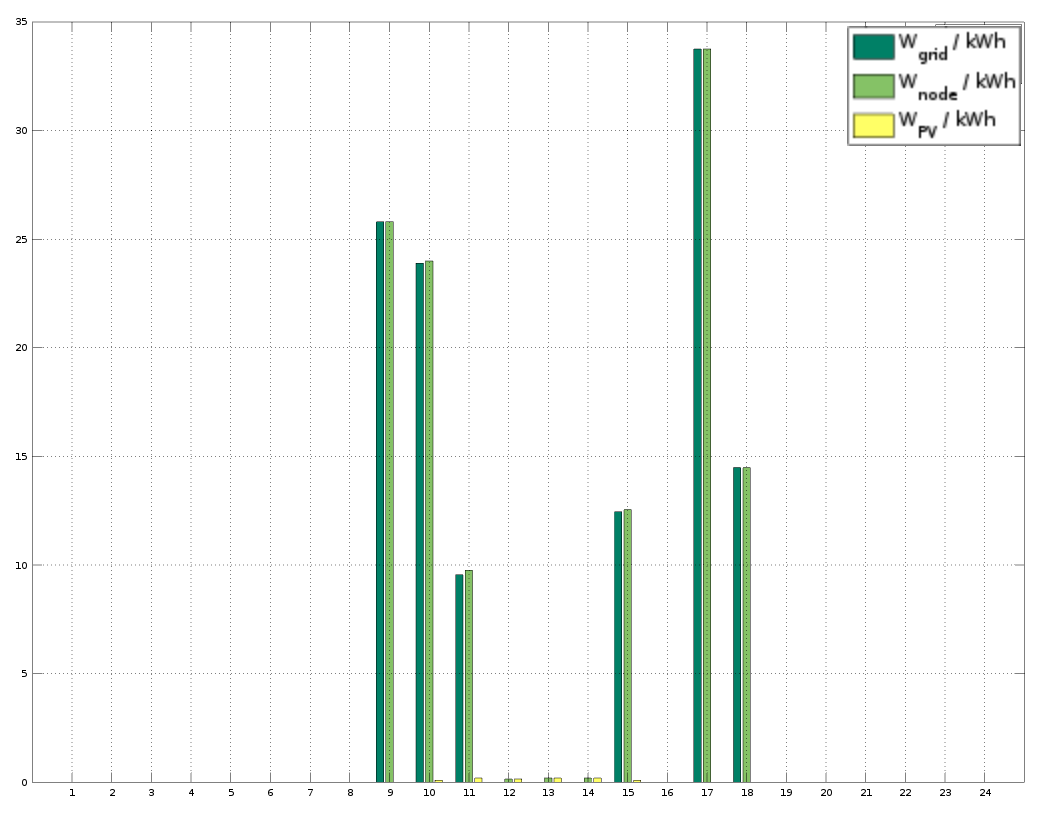
\includegraphics[width=\linewidth,height=8cm]{W_wc}
			\caption{Szenario Worst Case: Stündliche Energieflüsse über 24~h \\ 
            	des öffentlichen Netzes (grid) und der PV-Anlage (PV) im Erzeugerpfeilsystem \\
            	und der Ladeinfrastruktur (node) im Verbraucherpfeilsystem}
			\label{Abb:Sim_W_wc}
		\end{figure}

		\begin{figure}[h]
			\centering
			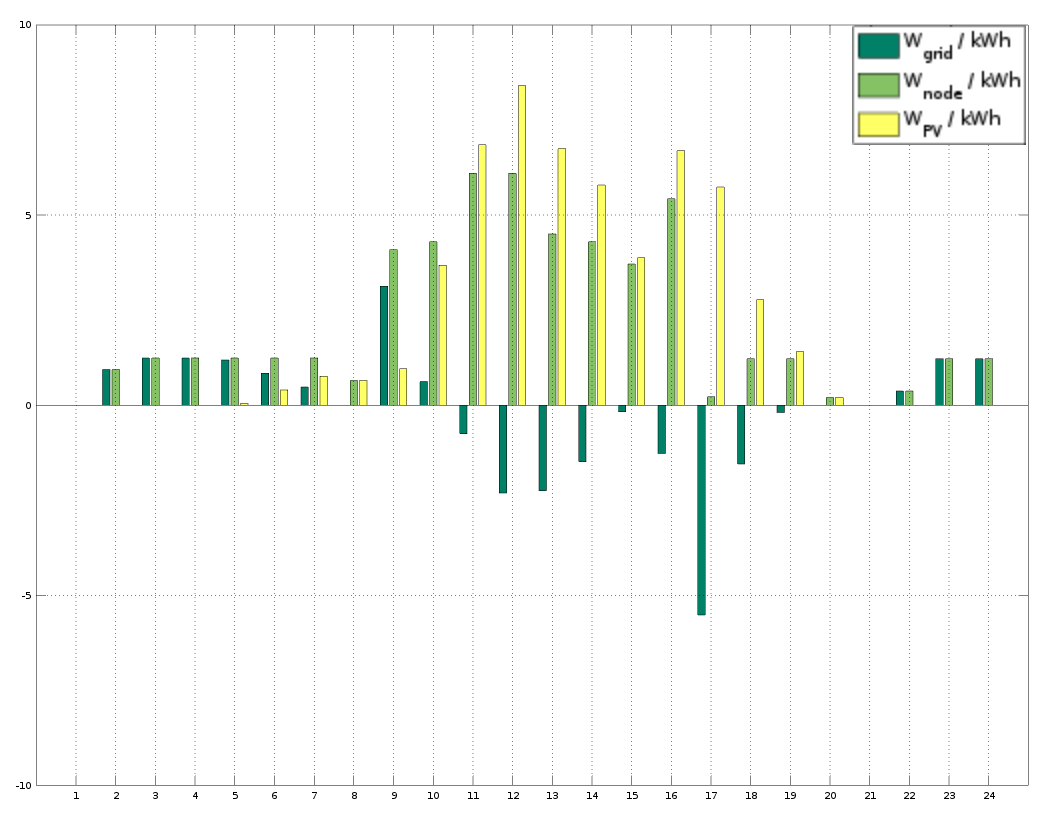
\includegraphics[width=\linewidth,height=8cm]{W_nc}
			\caption{Szenario Normal Case: Stündliche Energieflüsse über 24~h \\ 
            	des öffentlichen Netzes (grid) und der PV-Anlage (PV) im Erzeugerpfeilsystem \\
            	und der Ladeinfrastruktur (node) im Verbraucherpfeilsystem}
			\label{Abb:Sim_W_nc}
		\end{figure}

		\begin{figure}[h]
			\centering
			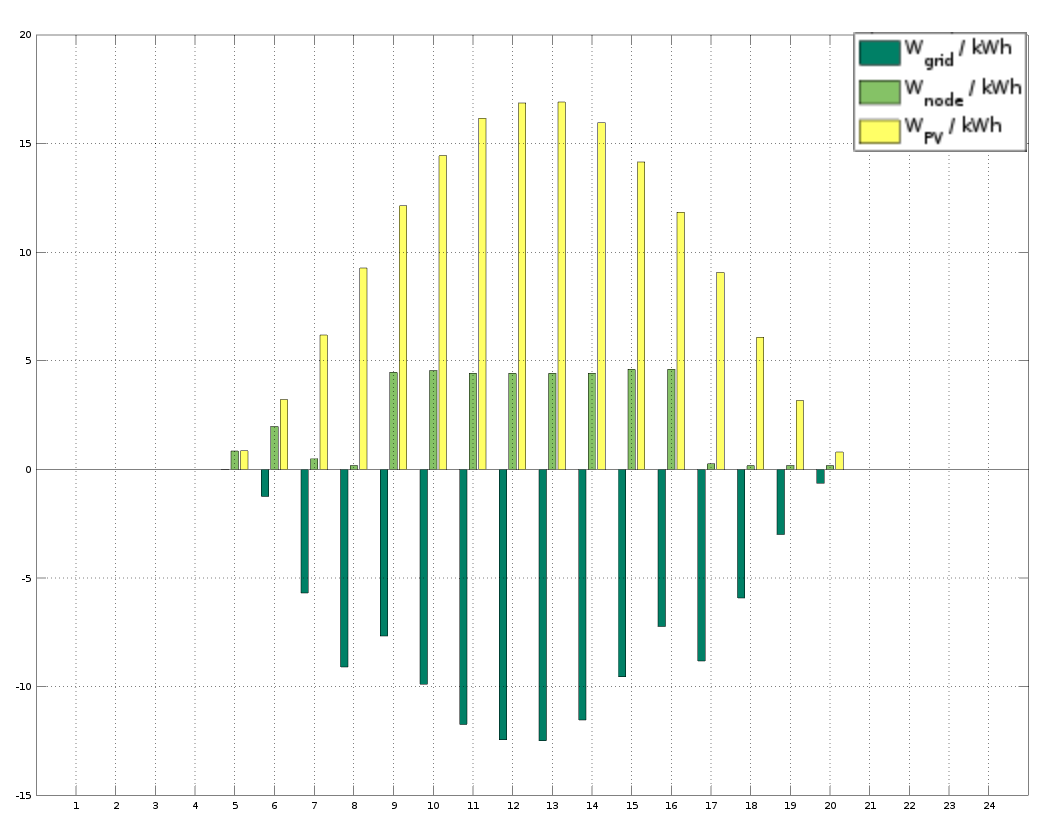
\includegraphics[width=\linewidth,height=8cm]{W_bc}
			\caption{Szenario Best Case: Stündliche Energieflüsse über 24~h \\ 
            	des öffentlichen Netzes (grid) und der PV-Anlage (PV) im Erzeugerpfeilsystem \\
            	und der Ladeinfrastruktur (node) im Verbraucherpfeilsystem}
			\label{Abb:Sim_W_bc}
		\end{figure}

		Für eine bessere Vergleichbarkeit aller drei Szenarien sind die stündlichen Energieflüsse der Ladeinfrastruktur (node) aller drei Szenarien in Abbildungen \ref{Abb:Sim_W_con_all}, der jeweilige Eigenenergieverbrauch der Ladeinfrastruktur in Abbildung \ref{Abb:Sim_W_con_self_all} und jene Energieflüsse des öffentlichen Versorgungsnetzes in Abbildung \ref{Abb:Sim_W_grid_all} dargestellt.\\
        
		\begin{figure}[h]
			\centering
			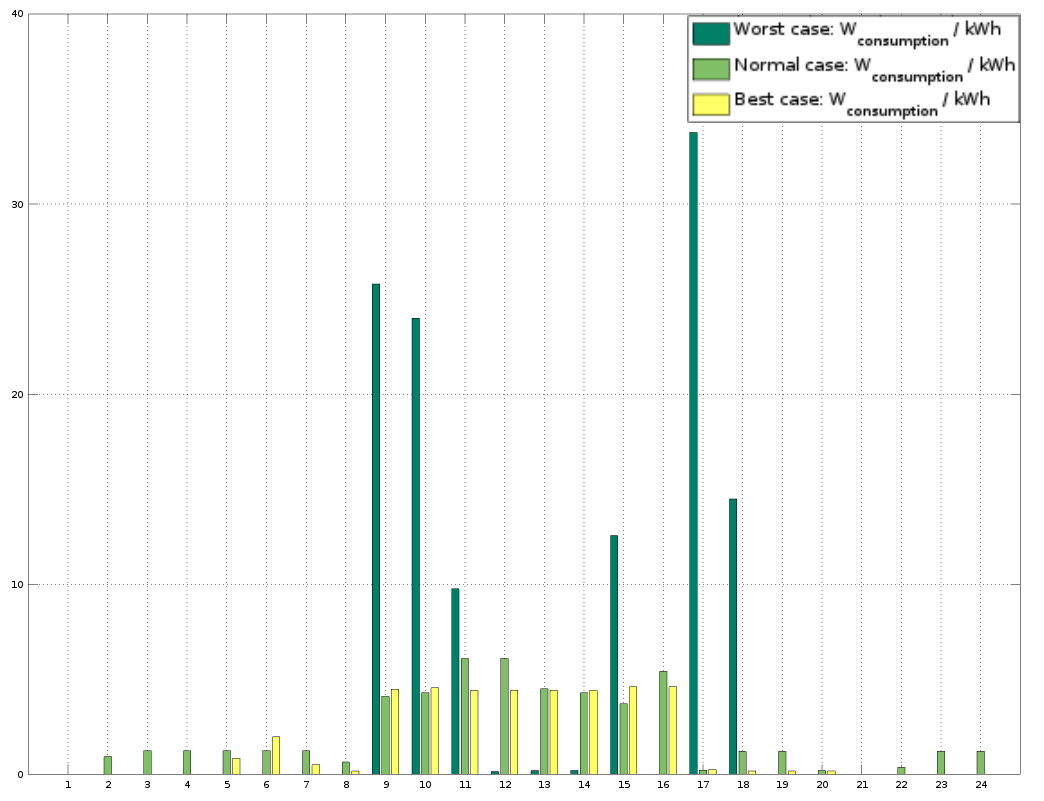
\includegraphics[width=\linewidth,height=8cm]{W_con_all}
			\caption{Stündlicher Energieverbrauch der Ladeinfrastruktur (node) über 24~h \\
            	in den Szenarien Worst Case, Normal Case und Best Case}
			\label{Abb:Sim_W_con_all}
		\end{figure}

		\begin{figure}[h]
			\centering
			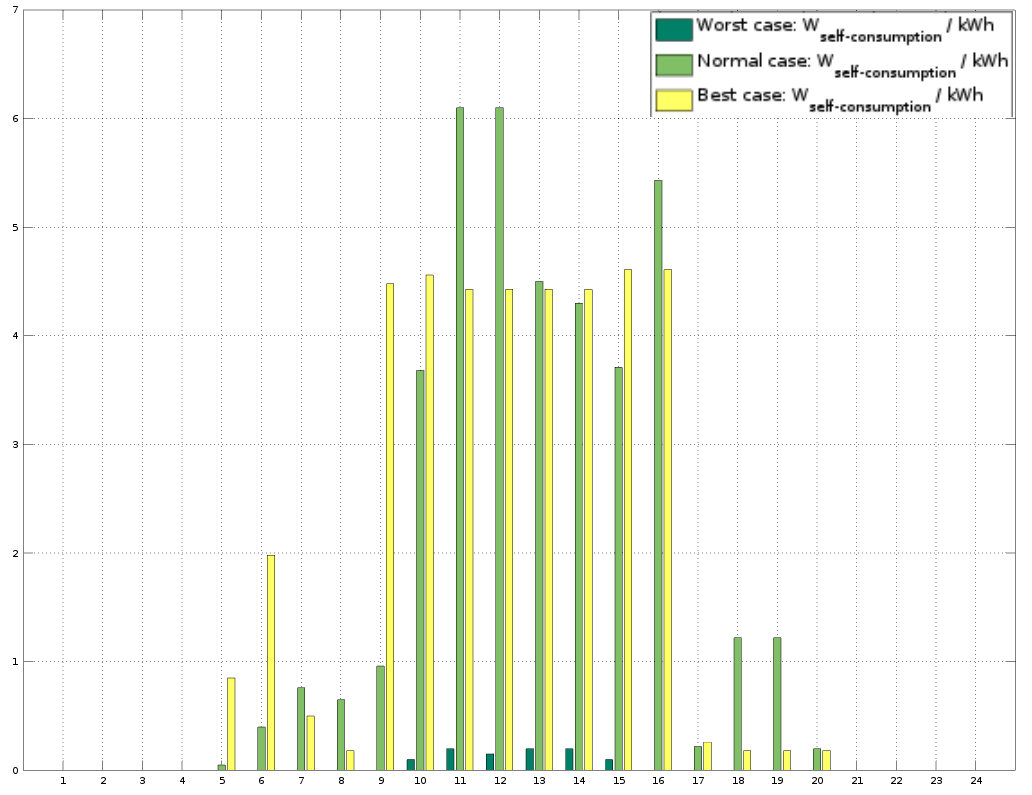
\includegraphics[width=\linewidth,height=8cm]{W_con_self_all}
			\caption{Stündlicher Eigenenergieverbrauch der Ladeinfrastruktur (node) an der PV-Erzeugung (PV) über 24~h \\
            	in den Szenarien Worst Case, Normal Case und Best Case}
			\label{Abb:Sim_W_con_self_all}
		\end{figure}

		\begin{figure}[h]
			\centering
			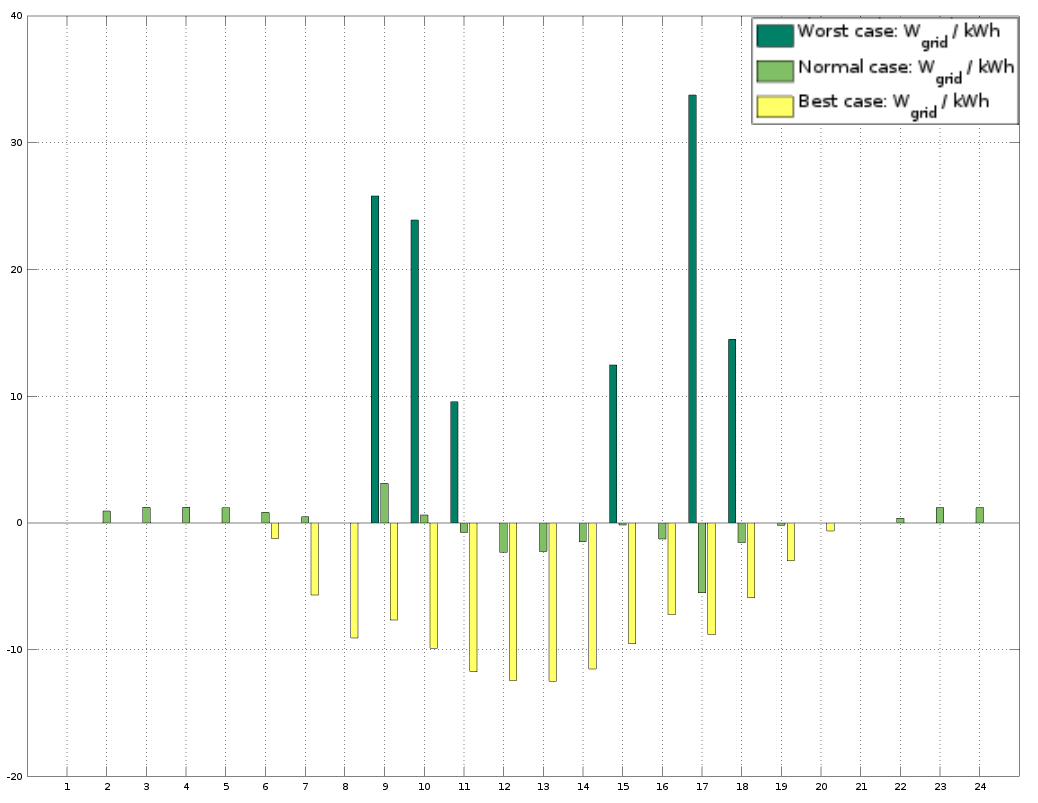
\includegraphics[width=\linewidth,height=8cm]{W_grid_all}
			\caption{Stündlicher Energiebezug vom öffentlichen Netz (grid) über 24~h\\
            	in den Szenarien Worst Case, Normal Case und Best Case}
			\label{Abb:Sim_W_grid_all}
		\end{figure}

	\subsection{Statistiken der einzelnen Szenarien}
		Für eine Gesamtbetrachtung werden die über den Simulationszeitraum summierten absoluten Werte $Gesamtverbrauch$, $Gesamterzeugung$, $Eigenverbrauch$ und die daraus abgeleitete Quotienten $Verh"altnis~~von~~Erzeugung~~zu~~Verbrauch$, $Autarkiegrad$ und $Eigenverbrauchsanteil$ für alle Szenarien ermittelt. \\
        
        Um den Einfluss der Pufferbatterie besser ermitteln zu können, werden zum Einen die Werte $Verbrauch~Pufferbatterie$ und $Erzeugung~Pufferbatterie$ über den Simulationszeitraum $T$ ermittelt. Zum Anderen werden noch drei Szenarien (WC0, NC0 und BC0) ohne Pufferbatterie aber sonst gleichen Bedingungen wie in den Szenarien WC, NC und BC simuliert und deren Statistiken erfasst. \\
        
        Alle Statistiken sind in Tabelle \ref{Tab:Sim_stats} für alle Szenarien gelistet und wurden für alle Szenarien mit Pufferbatterie mit Bereinigung des SoC berechnet. Die Pufferbatterie ist am Ende des Simulationszeitraums unterschiedlich stark geladen. Zur Bereinigung des SoC wird der theoretisch notwendige Eigenverbrauch oder die theoretisch notwendige Erzeugung für Eigenverbrauch zum Wiederherstellen des initialen SoC am Ende des Simulationszeitraums unter Berücksichtigung des (Ent-)Ladewirkungsgrades verwendet. 

        \begin{table}[h]
			\begin{tabularx}{\linewidth}{|X|c|c|c|}
				\hline 
                \multicolumn{4}{|c|}{\textbf{Statistiken Pufferbatterie-SoC bereinigt} } \\
                \hline 
														& \textbf{WC}  & \textbf{NC} & \textbf{BC}  \\ 
				\hline 
				\textbf{Verbrauch Pufferbatterie / kWh}				& 0,55		& 5,21		& 2,79 \\ 
				\hline 
				\textbf{Erzeugung Pufferbatterie / kWh} 			& 1,99		& 5,76		& 1,45 \\ 
				\hline 
				\textbf{Änderung SoC Pufferbatterie / kWh}			& -1,71		& -1,71		& 0,90 \\ 
				\hline 
				\textbf{Verbrauch Pufferbatterie* / kWh}			& 2,45		& 7,11		& 2,79 \\ 
				\hline 
				\textbf{Erzeugung Pufferbatterie* / kWh} 			& 1,99		& 5,76		& 2,26 \\ 
				\hline 
				\textbf{Gesamterzeugung* / kWh} 					& 0,96		& 55,00		& 157.18 \\ 
				\hline 
				\textbf{Gesamtverbrauch* / kWh}						& 122,84	& 53,89		& 39,57 \\ 
				\hline 
				\textbf{Eigenverbrauch* / kWh} 						& 0,96		& 39,51		& 40.38 \\ 
				\hline 
				\textbf{Verhältnis Erzeugung zu Verbrauch* / \%} 	& 0,79		& 105,78	& 389,25 \\ 
				\hline  
				\textbf{Eigenverbrauchsanteil* / \%}				& 100,00	& 71,85		& 25,69 \\ 
				\hline                
				\textbf{Autarkiegrad* / \%} 						& 0,78		& 73,32		& 100,00 \\ 
				\hline 
                \multicolumn{4}{|c|}{\textbf{Statistiken ohne Pufferbatterie} } \\
                \hline 
                										& \textbf{WC**}  & \textbf{NC**} & \textbf{BC**}  \\ 
				\hline 
				\textbf{Gesamtverbrauch / kWh}						& 122,38	& 52,54		& 39,04 \\ 
				\hline 
				\textbf{Eigenverbrauch / kWh} 						& 0,40		& 34,47		& 37,59 \\ 
				\hline 
				\textbf{Verhältnis Erzeugung zu Verbrauch / \%} 	& 0,78		& 104,67	& 402,66 \\ 
				\hline  
				\textbf{Eigenverbrauchsanteil / \%}					& 42,11		& 62,69		& 23,91 \\ 
				\hline                
				\textbf{Autarkiegrad / \%} 							& 0,33		& 65,61		& 96,29 \\ 
				\hline                
			\end{tabularx} 
			\caption{Statistiken der simulierten Szenarien Worst (WC), Normal (NC) und Best (BC) Case \\
            		*SoC der Pufferbatterie bereinigt mit SoC(Startzeit) = SoC(Endzeit) \\
                    **Szenarienbedingungen gleich WC, NC und BC ohne Verwendung einer Pufferbatterie}
			\label{Tab:Sim_stats} 
		\end{table}	



 % Externe Datei einbinden
\chapter{Ergebniszusammenfassung und Handlungsempfehlungen zur Auslegung der Anlage}
\label{Kap5}
In diesem Kapitel werden die Simulationsergebnisse zusammengefasst, verglichen und bewertet, um daraus Handlungsempfehlungen zur Dimensionierung und Betriebsweise der Energieverbundinsel abzuleiten.

\section{Zusammenfassung der Ergebnisse}
\label{Kap:Simulation_result}
	\textbf{Ertrag und Verbrauch}\\
	Die Wertebereiche für mögliche Ertrags- und Verbrauchsleistungen umfassen eine große Spannbreite. Das Ertragsprofil fluktuiert stark in Abhängigkeit des Wetters und der Tages- und Jahreszeit. Die Lastprofile der Szenarien unterscheiden sich stark in Abhängigkeit des Ladebedarfs, der Nutzungszeit und dem gewählten Lademodus. Dabei ist die Nutzungszeit in der Regel tagsüber für Angestellte, Studierende und Besuchende der Hochschule oder näheliegender Einrichtungen und nachts für Anwohnende. Der Tagesertrag der PV-Anlage mit 20,145 kWP schwankt von kleiner als 1~kWh im WC bis über 157~kWh bei einem Durchschnitt von 55~kWh. Der Gesamtverbrauch der aller drei Szenarien beträgt 122,38~kWh im WC, 52,54~kWh im NC und 39,04~kWh im BC. Das Verhältnis aus insgesamt erzeugter und durch Ladepunkte verbrauchter Energie beträgt in den Szenarien 0,78~$\%$ im WC, 104,67~$\%$ im NC und 402,66~$\%$ im BC.\\

	\textbf{Eigenverbrauchsanteil, Autarkiegrad und Einfluss der Pufferbatterie}\\
	Die Eigenverbrauchsanteile und Autarkiegrade lassen sich aus den Ertrags- und Verbrauchsprofilen sowie der Dimensionierung der Pufferbatterie errechnen. Der Eigenverbrauchsanteil der PV-Erzeugung mit (und ohne) Pufferbatterie beträgt jeweils 100~$\%$ (42,11~$\%$) im WC, ca. 71,85~$\%$ (62,69~$\%$) im NC und ca. 25,69~$\%$ (23,91~$\%$) im BC und der Autarkiegrad mit (und ohne) Pufferbatterie
0,78~$\%$ (0,33~$\%$) im WC, 73,32~$\%$ (65,61~$\%$) im NC und 100~$\%$ (96,29~$\%$) im BC. Die Pufferbatterie findet im WC am wenigsten und im NC am meisten Gebrauch. Den Eigenverbrauchsanteil beeinflusst die Pufferbatterie relativ gesehen am stärksten im WC trotz geringstem Verbrauch, da das Verhältnis von PV-Erzeugung zu Verbrauch deutlich kleiner ist als im NC und BC. Der Autarkiegrad wird durch die Pufferbatterie am stärksten im NC erhöht. Die Brutto Ladeenergie (und Netto Entladeenergie) der Pufferbatterie beträgt jeweils 0,55~kWh (1,99~kWh) im WC, 5,21~kWh (5,76~kWh) im NC und 2,79~kWh (1,45~kWh) im BC.\\

\section{Bewertung der Ergebnisse}
	\label{Kap:Simulation_conclusion}
	Die Simulationsergebnisse sind nur bedingt aussagekräftig, aufgrund der hohen Unsicherheit der Repräsentativität des modellierten Nutzungsverhaltens der Ladeinfrastruktur. Die zeitliche Auflösung von einer Stunde mittelt zudem Schwankungen des Ertragsprofils heraus. \\
    
	Die Pufferbatterie bietet an an Tagen extrem hoher oder niedriger PV-Erträge nur einen geringen Vorteil. Lediglich an normalen Tagen kommt sie mit mehr als einem Ladezyklus am Tag bemerkbar zum Gebrauch und verbessert den Autarkiegrad deutlich. Die potentielle Regelleistung durch intelligent gesteuerte Ladesequenzen ist verglichen mit der Pufferbatterie wesentlich größer und verlustärmer um ungünstige Lastspitzen zu vermeiden. \\    
    
\section{Handlungsempfehlung zur Auslegung und Betriebsweise der Anlage}
\label{Kap:Advice}
\subsection{Komponentenauswahl der Energieverbundinsel}
	Für die Ausarbeitung der Komponentenebene in SGAM zur Optimierung der Ladefinfrastruktur auf Energie- und Kosteneffizienz empfehlen sich folgende Punkte:
    \begin{itemize}
    	\item \underline{Prozesszone:}\\
        	Nutzung keiner Pufferbatterie aufgrund Nichtrentabilität und geringen Regelleistungspotential und für die Ladeinfrastruktur eine Neuauslegung der maximalen Übertragungsleistung am Anschlusspunkt der Ladeinfrastruktur auf ca. 22 bis 30~kW und an den drei Auto-Ladepunkte (mit Typ 2 Stecker) auf 1x22~kW AC und 2x11~kW AC  
        \item \underline{Feldzone:} \\
        	Konzipierung der Ladepunkte mit steuerbarem Laderegler und sicherer Kommunikationsmöglichkeit entweder mit zentralem EMS oder dezentral untereinander und mit Erzeugungsanlagen
	\end{itemize} 
%            - Verwendung keiner Pufferbatterie wegen Nichtrentabilität und geringem Potential für Regelleistung \\
%            - Neuauslegung der Begrenzung der Übertragungsleistung am Anschlusspunkt der Ladeinfrastruktur auf ca. 22 bis 30~kW \\
%            - Neuauslegung der drei Auto-Ladepunkte auf 1x22~kW AC und 2x11~kW AC mit Typ 2 Steckern       

\subsection{Energiemanagementkonzept}
	Für die Verbesserung des Energiemanagementkonzepts im SGAM empfehlen sich folgende Punkte:    
    \begin{itemize}
        \item \underline{Funktionsebene: Operationszone} \\ 
        	Entwicklung einer dynamischen Ladesteuerung mit Berücksichtigung sowohl der momentanen als auch prognostizierten erzeugten bzw. verbrauchten Leistung im Verbundnetz
		\item \underline{Kommunikations- und Informationsebene: Feld-, Stations- und Operationszone} \\ 
			Grundlegende Untersuchung von Möglichkeiten dezentralen Energiemangements ohne klassische Server-Client-Hierarchie durch eigenintelligent miteinander kommunizierende Geräte unter Anwendung von Distributed-Ledger-Technologien verteilter Rechennetzwerke wie z.B. Technologien auf Basis von Blockchains wie Etherum, auf Basis von Blockchainabwandlungen wie der Tangle von IOTA oder auf Basis von Hashgraphen
        \item \underline{Informations- und Funktionsebene: Prozess- Feld-, Stations- und Operationszone} \\ 
        	Erstellung einer Testumgebung mit Datenmodellen und Energiemanagementalgorithmus möglichst in einer Sprache, womit sich die Steueralgorithmen der Testumgebung möglichst einfach implementieren lassen z.B. durch Verwendung des Datenprotokolls SPINE von EEBUS
    \end{itemize}
    
    
\section{Ausblick}
\label{Kap:Perspektive}
	Auf weite Sicht lässt sich die geplante Energieverbundinsel auf mehr als die PV-Anlage und die Ladeinfrastruktur erweitern. 
	\begin{itemize}
        \item \underline{Komponentenebene: Prozesszone:} \\
        	- Berücksichtigung des Gesamtverbrauchs im Hochschulnetz \\
        	- Integration von mehr vorhandenen energietechnisch relevanten Geräten in die Energieverbundinsel, z.B. Lüftungssysteme und Boiler der Hochschule\\
        	- Untersuchung der Ausbaumöglichkeiten von weiteren Erzeugungsanlagen wie weiteren PV-Anlagen und Mini-Windkraftanlagen \\
        	- Nähere Untersuchung zum Ausbaupotential weiterer Speichermöglichkeiten z.B. durch Verwendung von Wasserstoffelektrolyse und einer Brennstoffzelle
        \item \underline{Ebenenübergreifend:} \\ 
        	Ausbau der Energieverbundinsel zum zentral gesteuerten virtuellen Kraftwerk zur Bereitstellung von Regelleistung für das elektrische Versorgungsnetz oder Ausbau der Infrastruktur für intelligente Anbindung von Einzelgeräten zur Bereitstellung von Regelleistung durch Einzelgeräte als virtuelles Mini-Kraftwerk 
	\end{itemize}
    
 % Externe Datei einbinden
\chapter{Fazit}
\label{Kap6}
% Ziel und Konzept Energieverbundinsel
	Das Ziel der Studie ist es, die Energieflüsse innerhalb der geplanten Energieverbundinsel zu optimieren. Im Folgenden wird eine Zusammenfassung der Studienergebnisse und eine kritische Schlussbemerkung zur verwendeten Methodik gegeben. \\

% Konzept Energieverbundinsel
    Das Konzept der Energieverbundinsel mit Ladeinfrastruktur, PV-Anlage und Pufferbatterie wurde in die Komponenten-, Informations- und Funktionsebene des Smart Grid Architecture Model eingeordnet, um das Projekt möglichst gut in Teilbereiche zu gliedern und eine bessere Übersicht für zukünftige Entwicklungen zu schaffen. Es wurde ein möglichst modulares Modell von einer steuerbaren Ladeinfrastruktur mit PV-Anlage und Pufferbatterie erstellt, das leicht erweitert werden kann. \\

% Konzept Energiemanagement und Simlation(stool)
	Das erstellte Energiemanagementkonzept zur Optimierung der Energieflüsse ist ein ausbaubares Grundgerüst, kann funktional erweitert und auf zusätzliche Betriebsmittel ausgeweitet werden. Es wurde für verschiedene Beispielszenarien in einer programmierten Simulationsumgebung getestet, welche für weitere Untersuchungen genutzt und verbessert werden kann. Aus den Simulationsergebnissen wurden Handlungsempfehlungen für die Auswahl der Komponenten der Ladeinfrastruktur und deren Dimensionierung und Betriebsweise abgeleitet. \\
    
% Handlungsempfehlung und Ausblick    
    Es wird von einer Auslegung der Ladeinfrastruktur für Schnellladungen bis 50~kW abgeraten, da in der Regel längere Ladezeiten während der Arbeit oder zu Hause möglich sind. Für die Betriebsweise empfiehlt es sich, den Fokus auf die Entwicklung intelligenter Ladesequenzen zu legen, statt in teure Batteriespeicher zu investieren. Allgemein rät es sich, das gesamte Hochschulnetz in die Energieverbundinsel mit einzubeziehen und zusätzliche oder bestehende Betriebsmittel ins Energiemanagementsystem (EMS) zu integrieren. Als mögliche Stoßrichtung für Entwicklungen auf lange Sicht, wurde im Ausblick die Möglichkeit eines Ausbaus der Energieverbundinsel zum virtuellen Kraftwerk skizziert, wodurch Regelleistung für das Versorgungsnetz bereit gestellt werden könnte. Grundsätzlich wird geraten vor der Implementation eines EMS, das Potential verschiedener zentraler und dezentraler Kommunikationsansätze zu vergleichen. \\

% Kritische Betrachtung
	Kritisch anzumerken ist zum Einen, dass sich die Abgrenzung der Themenstellung als ungünstig umfassend erwies, sodass der Zeitaufwand auf 4 Monate erweitert werden musste und an einigen Stellen dennoch unerwünschte Abstriche gemacht werden mussten, wodurch die gewählte Aufgabenstellung nicht im vollen Umfang gelöst wurde. Zum Anderen hat sich gezeigt, dass sich die Kosten- und Energieeffizienz besser als Bewertungskriterium für verlustbehaftete Speichermöglichkeiten wie der Pufferbatterie eignen als der alleinige Vergleich erreichbarer Autarkiegrade. \\
    
% Kritische Betrachtung: Abgrenzung und Priorisierung
	Der Arbeitsaufwand zum Programmieren der halbautomatisierten Analyse regionaler Globalstrahlungsdaten zur Erstellung von PV-Ertragsprofilen wurde unterschätzt und ist unverhältnismäßig hoch. Die einmalige Auswahl jeweils eines Tages mit maximaler, durchschnittlicher und minimaler Globalstrahlung konnte mithilfe eines herkömmlichen Tabellenkalkulators schneller durchgeführt werden. Zudem hätte in der Simulationsumgebung aufgrund der untersuchten Nicht-Rentabilität der gewählten Pufferbatterie die Implementation flexibler Ladesequenzen höher priorisiert werden sollen als die Implementation der Pufferbatterie. \\
    
    Mit der Studie konnte die Zielsetzung trotz umfassender Arbeitsplanung erreicht werden. Darüber hinaus wurden Kenntnisse zu Smart Grid Architekturen, Energiemanagementkonzepten, dem Aufbau einer Ladeinfrastruktur, Programmierkenntnisse in Matlab und Methoden wissenschaftlichen Arbeitens erworben beziehungsweise ausgeweitet.



    
    
    %Es bestimmt die Nennleistung von Ladepunkten maximal oder kontinuierlich über einen Anschlusszeitraum und die Nennleistung der Pufferbatterie so, dass möglichst viel PV-Ertragsüberschüsse gepuffert und bei Bedarf bereit gestellt werden. Im Falle, dass die Gesamtsumme aller Nennleistungen von Geräten an einem Netzknoten die zulässigen Übertragungsleistung zum nächsten verbundenen Netzknoten überschreitet, werden stufenweise alle Geräte eines Netzknotens mit identischer Priorität gleichmäßig gedrosselt, um möglichst viel der unzulässigen Nennleistung auszugleichen. \\

% Simulation, Auswertung, Handlungsempfehlungen Komponenten und Energiemanagement
     % Externe Datei einbinden
% ------------------------------------------------------------------

\label{lastpage}

% Neue Seite
\cleardoublepage

% Backmatter mit normalem Zeilenabstand setzen
\singlespacing

% Römische Ziffern für die "Back-Matter", fortlaufend mit "Front-Matter"
\pagenumbering{roman}
\setcounter{page}{\value{frontmatterpage}}

% Literaturverzeichnis erzeugen
\begin{flushleft}
\printbibliography
\end{flushleft}

% Tabellenverzeichnis erzeugen
\cleardoublepage
\phantomsection
\addcontentsline{toc}{chapter}{\hsmalistoftables}
\listoftables

% Abbildungsverzeichnis erzeugen
\cleardoublepage
\phantomsection
\addcontentsline{toc}{chapter}{\hsmalistoffigures}
\listoffigures

% Listingverzeichnis erzeugen
\cleardoublepage
\phantomsection
\addcontentsline{toc}{chapter}{\hsmalistings}
\lstlistoflistings

% Index ausgeben. Wenn Sie keinen Index haben, entfernen Sie einfach
% diesen Teil.
%\cleardoublepage
%\phantomsection
%\addcontentsline{toc}{chapter}{\hsmaindex}
%\printindex

% Anhang. Wenn Sie keinen Anhang haben, entfernen Sie einfach
% diesen Teil.
\appendix
\chapter{Erster Anhang - Technische Spezifikationen}
\label{Kap:Anhang1}
In diesem Anhang sind technische Spezifikationen und eine Grafik mit Entwicklung von Wirkungsgraden verschiedener PV-Technologien gelistet. Die Tabellen und abbildungen gliedern sich in die folgenden Sektionen.

\section{Entwicklung verschiedener PV-Technologien}

\begin{landscape}
  \begin{figure}[h]
      \centering
      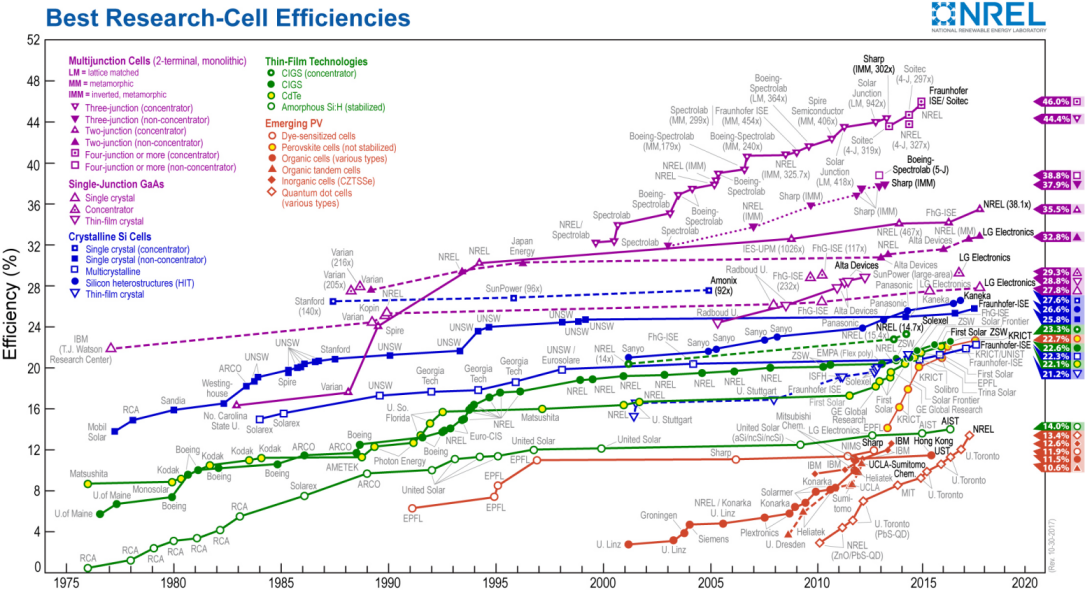
\includegraphics[width=\linewidth]{NREL_PV_efficiency_1975_2020}
      \caption{Entwicklung der Wirkungsgrade verschiedener Solarzellentechnologien \cite{Comparison_Batteries_2015}, \cite{NREL_PV_eta}}
      \label{Abb:Vgl_PV_eta}
  \end{figure}
\end{landscape}

\begin{landscape}
\section{Steckersysteme und Ladetechniken für Elektro-Autos}
  \begin{table}[h]
      \centering
      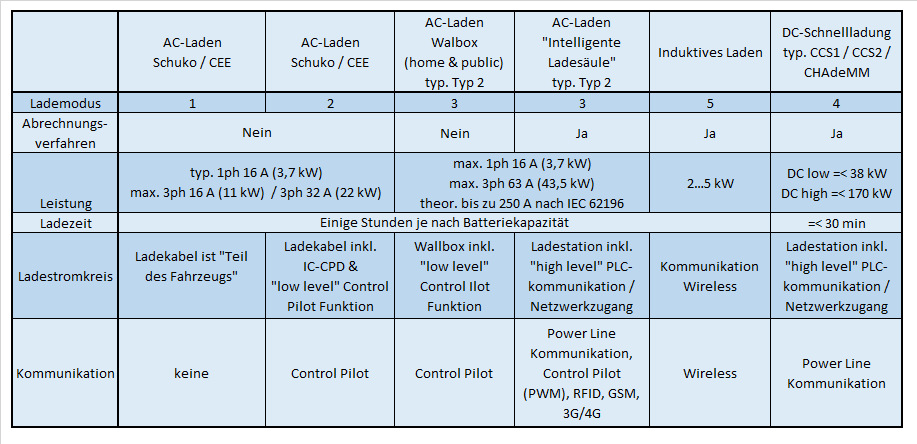
\includegraphics[width=0.9\linewidth]{Vergleich_Ladesysteme_EAuto}
      \caption{Vergleich verschiedener Ladesysteme für E-Autos \cite[S.15]{Emobility_StatusQuo_2016}} 
      \label{Tab:Vgl_Ladesysteme_EAuto}
  \end{table}
\end{landscape}

  \begin{table}[h]
      \centering
      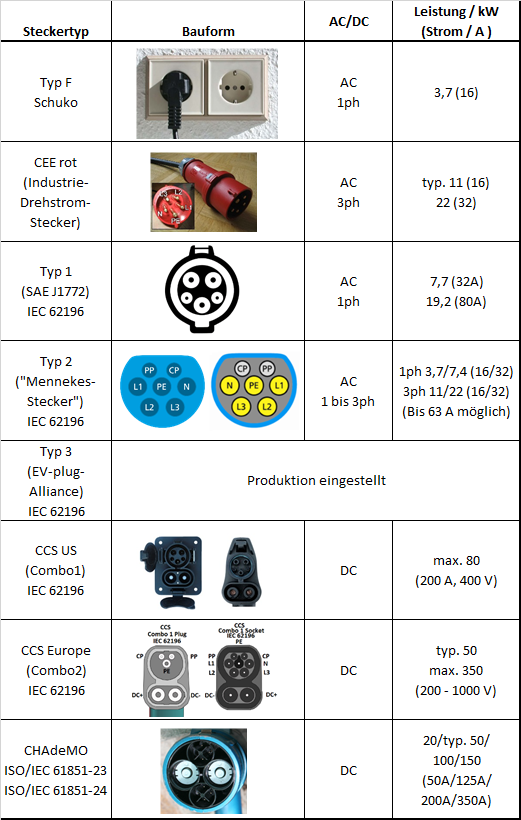
\includegraphics[width=14cm]{Stecker_typentabelle}
      \caption{Vergleich verschiedener standardisierter Steckervorrichtungen; Bildquellen:\cite{Abb_Steck_Schuko}\cite{Abb_Steck_CEE}\cite{Abb_Steck_Typ1}\cite{Abb_Steck_Typ2}\cite{Abb_Steck_Combo1}\cite{Abb_Steck_Combo2}\cite{Abb_Steck_CHAdeMO}}
      \label{Tab:Vgl_Steckervorrichtungen}
  \end{table}	

\begin{landscape}
\section{EEBUS Spezifikation}
  \begin{figure}[h]
      \centering
      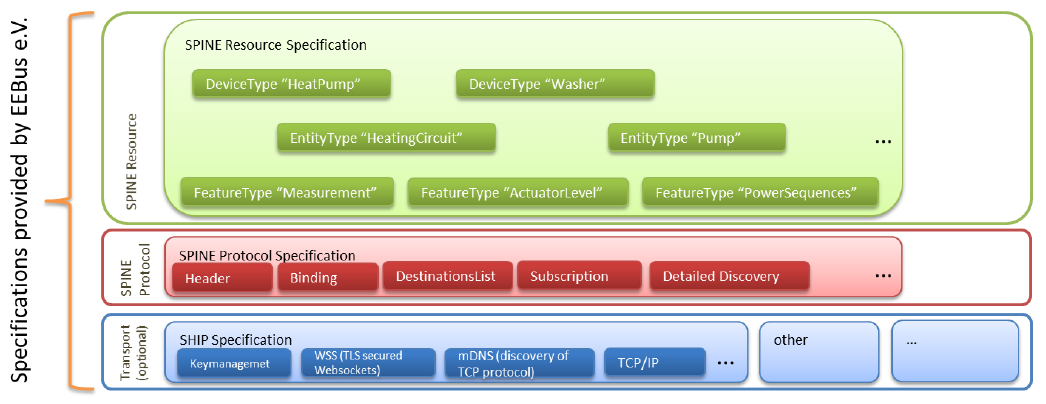
\includegraphics[width=\linewidth]{EEBUS_Spec}
      \caption{EEBUS Spezifikation im Detail \cite[S.5]{EEBUS_Intro}}
      \label{Abb:EEBUS_Spec}
  \end{figure}			
\end{landscape}                

\section{Herstellerangaben zu PV-Anlage, PV-Wechselrichter und Pufferbatterie}
\label{Kap:datasheet_pv_wr}

  \begin{figure}[h] 
      \centering
      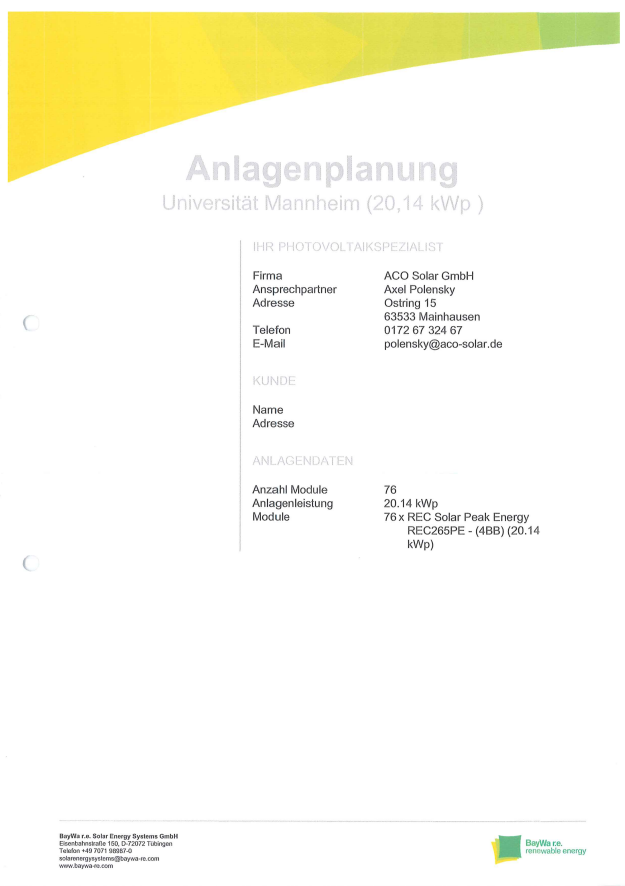
\includegraphics[width=0.8\linewidth]{datasheet_pv_1}
      \caption{Spezifikation der PV-Anlage auf Gebäude C der Hochschule Mannheim, Ausschnitt der Anlagenplanung} 
      \label{Abb:datasheet_pv_1}
  \end{figure} 	

  \begin{figure}[h] 
      \centering
      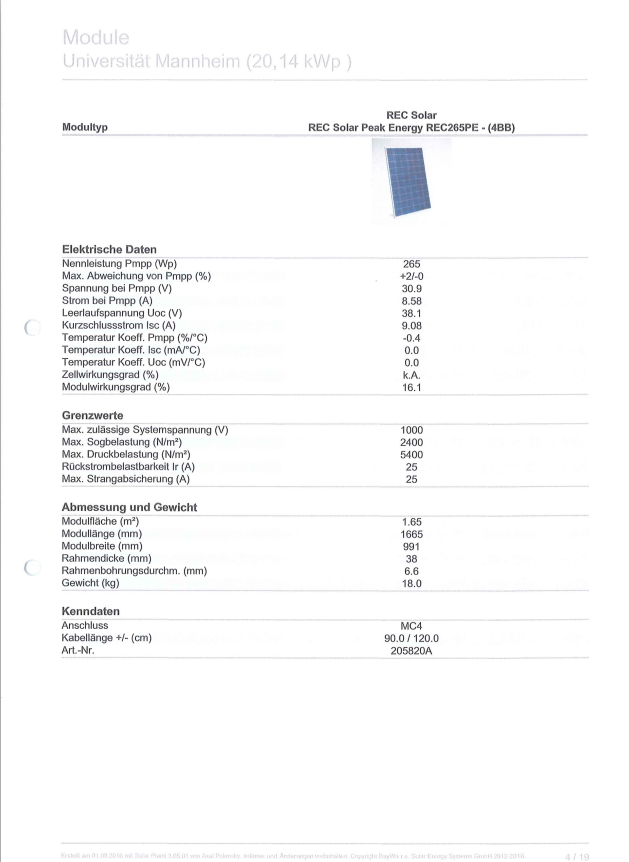
\includegraphics[width=\linewidth]{datasheet_pv_2}
      \caption{Spezifikation der PV-Anlage auf Gebäude C der Hochschule Mannheim, Ausschnitt der Anlagenplanung: Kenndaten des Moduls REC Solar Peak Energy REC265PE} 
      \label{Abb:datasheet_pv_2}
  \end{figure} 	

  \begin{figure}[h] 
      \centering
      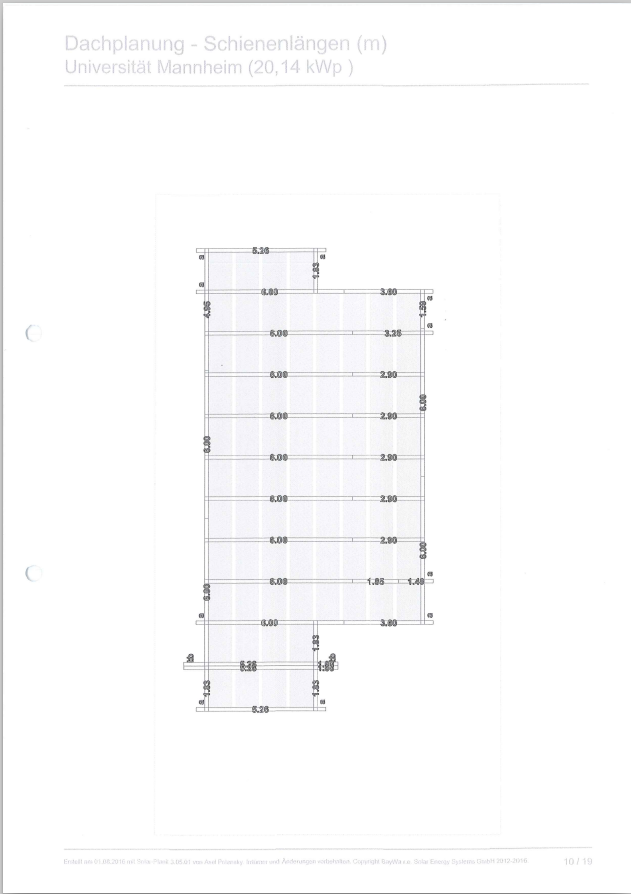
\includegraphics[width=\linewidth]{datasheet_pv_3}
      \caption{Spezifikation der PV-Anlage auf Gebäude C der Hochschule Mannheim, \\ Ausschnitt der Anlagenplanung: Dachplanung - Schienenlänge, Modulpositionen \\ (Himmelsrichtung Norden, oben im Bild)} 
      \label{Abb:datasheet_pv_3}
  \end{figure} 	

  \begin{figure}[h] 
      \centering
      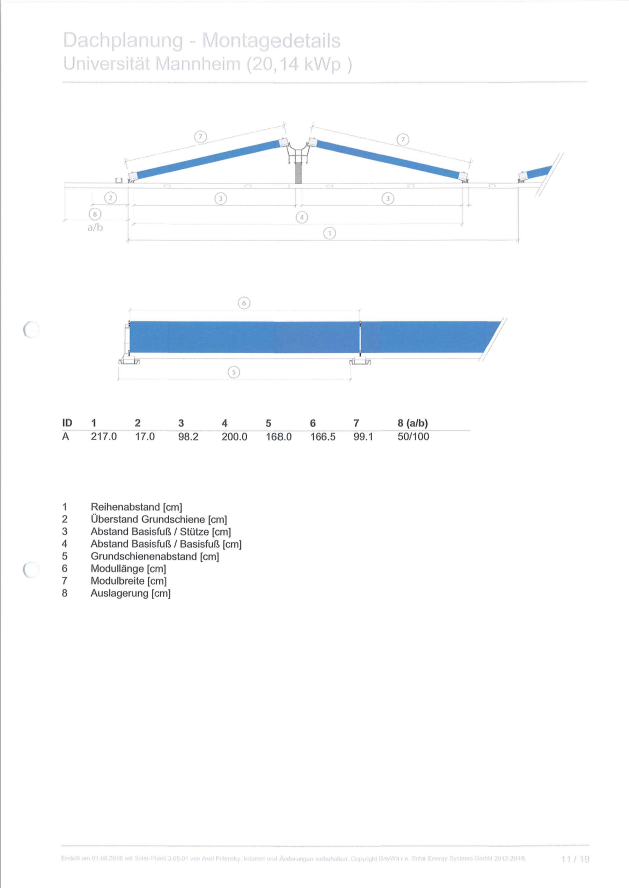
\includegraphics[width=\linewidth]{datasheet_pv_4}
      \caption{Spezifikation der PV-Anlage auf Gebäude C der Hochschule Mannheim, \\ Ausschnitt der Anlagenplanung: Dachplanung - Montagedetails, Modulneigung \\ (Westen links, Osten rechts im Bild)} 
      \label{Abb:datasheet_pv_4}
  \end{figure} 	

  \begin{figure}[h] 
      \centering
      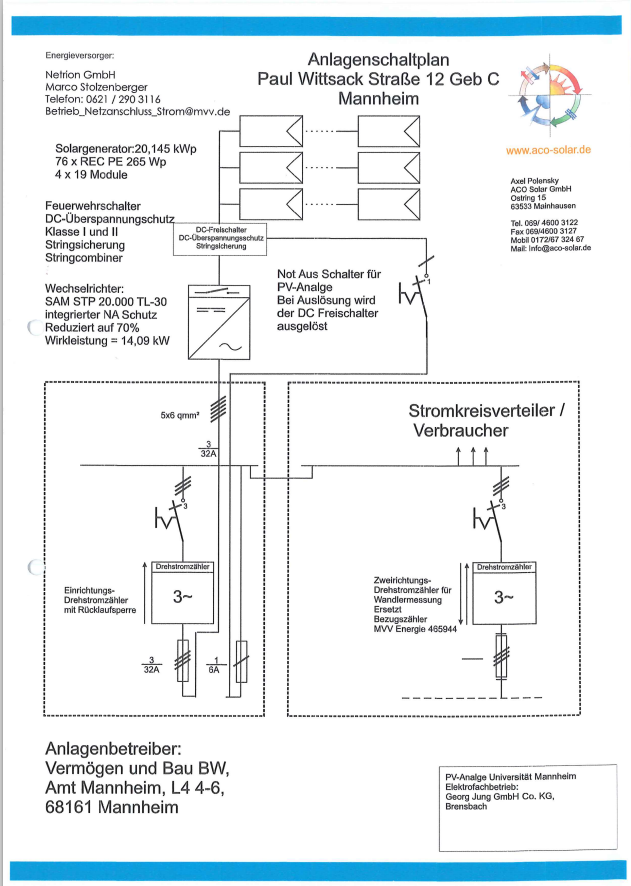
\includegraphics[width=\linewidth]{datasheet_pv_5}
      \caption{Spezifikation der PV-Anlage auf Gebäude C der Hochschule Mannheim, \\ Ausschnitt der Anlagenplanung: Anlagenschaltplan} 
      \label{Abb:datasheet_pv_5}
  \end{figure} 	

  \begin{figure}[h] 
      \centering
      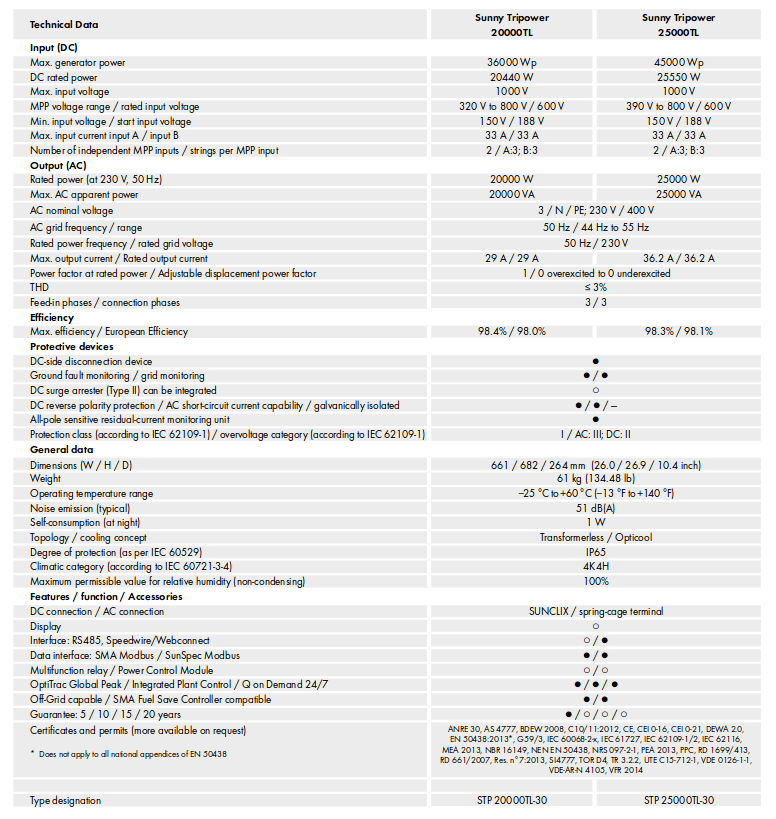
\includegraphics[width=\linewidth]{datasheet_wr}
      \caption{Spezifikation des PV-Wechselrichters, technische Herstellerangaben \cite{spec_SMA}} 
      \label{Abb:datasheet_wr}
  \end{figure} 	

  \begin{figure}[h] 
      \centering
      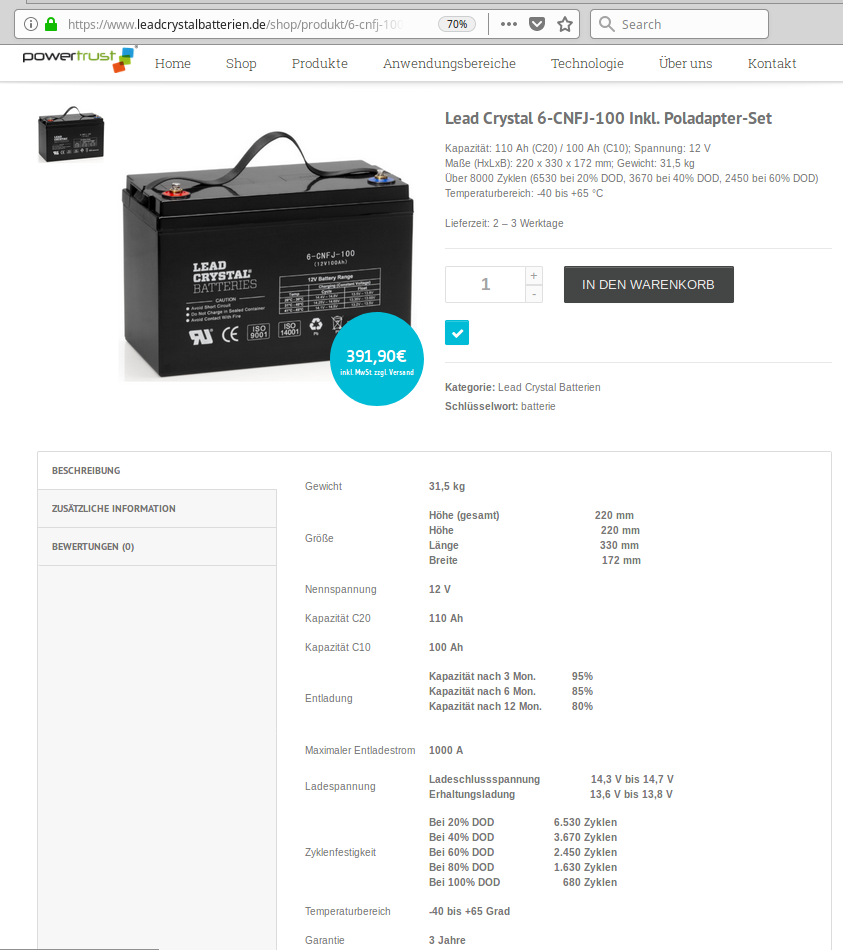
\includegraphics[width=\linewidth]{datasheet_akku}
      \caption{Spezifikation des Bleikristallakkus Lead Crystal 6-CNFJ-100 inkl. Poladapter-Set des Herstellers $\text{Lead Crystal}^{\textsuperscript{\textregistered}} ~\text{Batteries}$ \cite{spec_battery_buffer}}   
      \label{Abb:datasheet_akku}
  \end{figure} 	

  \begin{figure}[h] 
      \centering
      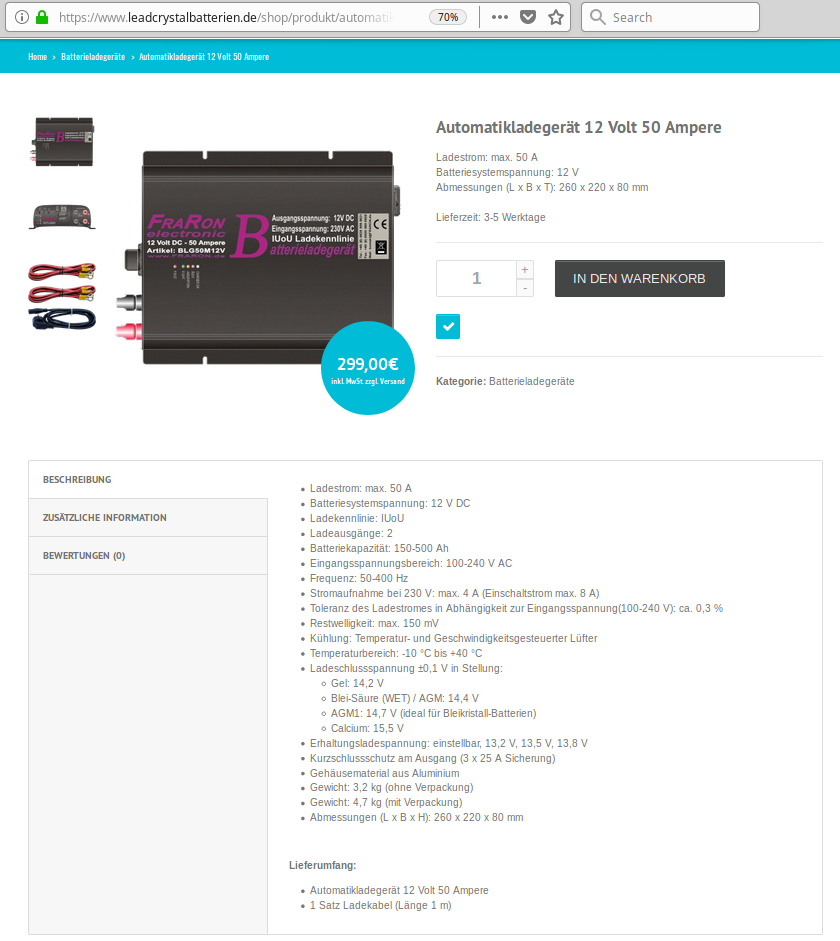
\includegraphics[width=\linewidth]{datasheet_laderegler}
      \caption{Spezifikation des Automatikladegeräts 12 Volt 50 Ampere des Herstellers Fraron \cite{spec_laderegler}} 
      \label{Abb:datasheet_laderegler}
  \end{figure} 	

\section{Projektplanung Gantt Chart}
\begin{landscape}
  \begin{figure}[h] 
      \centering
      \includegraphics[width=0.8\linewidth]{Projektplanung}
      \caption{Projektplanung mit Gantt project}
      \label{Abb:gantt}
  \end{figure} 	
\end{landscape} % Tabellen, Datenblätter
\chapter{Zweiter Anhang - Ermittlung des PV-Ertrags anhand der Globalstrahlung}
\label{Kap:Anhang2}
Der Inhalt dieses Kapitels zeigt die Berechnung von PV-Erträgen bei senkrecht auf die Modulfläche eintreffender Globalstrahlung. Außerdem wird der Rechenweg für die Bestimmung des senkrecht auf eine geneigte Fläche treffende Globalstrahlung an der senkrecht auf den Grund eintreffenden Globalstrahlung gezeigt.

  \section{PV-Ertrag bei anhand senkrecht auf die Modulfläche eintreffender Globalstrahlung bestimmen}
      \label{Kap:PV_global}
      Die erzeugte DC-Leistung $P_{PV,DC}$ berechnet sich aus dem Wirkungsgrad $\eta_{PV}$ der Zellen, der Kollektorfläche $A$ und der senkrecht auf die geneigte Modulfläche treffende Globalstrahlung $G_{0,g}$ mit der Kollektorfläche $A$.
	
      \begin{equation}
          P_{PV,DC} = \eta_{PV} \cdot G_{0,g} \cdot A
          \label{Eq:PV_Pdc}
      \end{equation}

      Der Wirkungsgrad $\eta_{PV}$ kann anhand der Peakleistung $P_p$ bestimmt werden.

      \begin{equation}
          \eta_{PV} = \frac{\frac{P_p}{A}}{G_{STC}} = \frac{\frac{P_p}{A}}{1000 \frac{W}{m^2}}
          \label{Eq:PV_eta}
      \end{equation}

      Die Ausgangsleistung des PV-Wechselrichters $P_{PV,AC}$ wird wie folgt berechnet.

      \begin{equation}
          P_{PV,AC} = \eta_{WR} \cdot P_{PV} = \eta_{WR} \cdot \eta_{PV} \cdot G_{0,g} \cdot A
          \label{Eq:PV_Pac}
      \end{equation}

	\section{Bestimmung der senkrecht auf eine geneigte Modulfläche eintreffenden Globalstrahlung}	
    	\label{Kap:G0g}
		Die vertikal auf eine geneigte Modulfläche eintreffende Globalstrahlung $G_{0,g}$ kann anhand der senkrecht auf den Grund treffenden Globalstrahlung $G_0$ gemäß Gleichung \ref{Eq:G0g} und \ref{Eq:cospsi} mit den in Tabelle \ref{Tab:sonnenwinkel} sowie den Abbildungen \ref{Abb:sonnenwinkel1} und \ref{Abb:sonnenwinkel2} definierten Winkelgrößen bestimmt werden.\cite{REN2}
        
      \begin{equation}
          G_{0,g} = G_0 \cdot cos(\psi)	
          \label{Eq:G0g}
      \end{equation}
      mit der Kosinusfunktion des Einfallswinkels $\psi$ nach folgender Gleichung:
      \begin{multline}
          cos(\psi) = (cos(\alpha) sin(\Phi) - sin(\alpha) cos(\Phi) cos(\beta)) sin(\delta) + \\
          ((cos(\alpha) cos(\Phi) + sin(\alpha) sin(\Phi) cos(\beta)) cos(\delta) cos(t) + \\ 
          sin(\alpha) sin(\beta) cos(\delta) sin(t) 
          \label{Eq:cospsi}
      \end{multline}

      "Die Deklination $\delta$ schwankt aufgrund der scheinbaren Sonnenbewegung um $\pm 23,450 {^\circ}$"\cite{REN2} und kann folgendermaßen berechnet werden, wobei d der Tag des Jahres, vom 1. Januar aus gezählt ist: \\ 
      \begin{equation}
          \delta = -23,45^{\circ} \cdot cos(360^{\circ} /365,25^{\circ} (d+10)) 
      \end{equation}

      Der Stundenwinkel t lässt sich aus der Rotationsgeschwindigkeit der Erde ermitteln.
      \begin{equation}
          15\degree/h (12h - WOZ) ~\text{dabei ist}~ WOZ = GZ + 4 min \cdot (\lambda_0 - \lambda) - Z
      \end{equation} 
      $ \text{und } Z/min = -7,66 sin(x) - 9,87 sin( 2x + 24,99\degree + 3,83\degree sin(x))$ \\
      $ \text{mit }x = 0,9856\degree d-2,72\degree$ \\

      Die wahre Ortszeit WOZ (Sonnenzeit) kann sich von der gesetzlich geregelten Zeit GZ (Ortszeit) je nach Ortslage und Jahreszeit unterscheiden. Die Ortszeit ist auf einen Längenmeridian $\lambda_0$ bezogen (z.B. MEZ: Bezungsmeridian $\lambda_0 = -15\degree$). \\
	
	
	\begin{table}[h]
		\begin{tabular}{|c|l|} %ggf. Mitte auch zentrieren
			\hline 
			Zeichen & Definition \\ 
			\hline 
			$\alpha \quad[$\degree$] $ & Neigungswinkel (gegen Horizontale)  \\ 
			\hline 
			$\beta \quad [$\degree$] $ & Azimutwinkel (Ost-West-Orientierung) (Empfangsfläche) \\ 
			\hline 
			$\delta \quad [$\degree$] $ & Deklination, Winkelabstand des Sonnenhöchststands vom Himmelsäquator  \\ 
			\hline 
			$\lambda \quad [$\degree$] $ & geographische Länge (Meridian)  \\ 
			\hline
			$\psi \quad [$\degree$] $ & Einfallswinkel (zwischen Strahlungsrichtung \& Flächennormalen)  \\ 
			\hline 
			$\Phi \quad [$\degree$] $ & geographische Breite  \\ 
			\hline 
			$t \quad [$\degree$] $ & Stundenwinkel (Sonnenstand) \\ 
			\hline 
		\end{tabular} 
		\caption{Beschreibung der Winkel um die Position der Erde zur Sonne zu beschreiben}
		\label{Tab:sonnenwinkel}
	\end{table}

\begin{landscape}
	\begin{figure}[h]
		\centering
		\includegraphics[width=\linewidth]{Strahlungswinkel_Sonne1}
		\caption{Relevante beschreibende Winkelgrößen, welche die Bewegung der Erde um die Sonne beschreiben und so für $G_{0,g}$ entscheidend sind. Die Variablen des Horizonts- und des Äquator-Koordinatensystems (links und mittig). Rechts die Aufteilung im Horizont-Koordinatensystem für die nördliche (Zenit) und südliche (Nadir) Halbkugel.\cite{REN2}}
		\label{Abb:sonnenwinkel1}
	\end{figure}
	
	\begin{figure}[h]
		\centering
		\includegraphics[width=\linewidth]{Strahlungswinkel_Sonne2}
		\caption{Relevante beschreibende Winkelgrößen, welche die Bewegung der Erde um die Sonne beschreiben und so für $G_{0,g}$ entscheidend sind. Hier Ekliptik und Himmelsäquator bzw. Horizont \cite{REN2}}
		\label{Abb:sonnenwinkel2}
	\end{figure}
\end{landscape}
         % Globalstrahlung umrechnen
\chapter{Dritter Anhang - Aufbau des SGAM Frameworks}
\label{Kap:SGAM_aufbau}

\section{Grundlegender Aufbau des SGAM Frameworks}
	Das \ac{SGAM} besteht aus Interoperabilitäts-Ebenen (Layers), physikalischen Domänen (Domains) entlang der Energieumwandlungskette und funktionaler Zonen (Zones) des Prozessmanagements, die in Abb. \ref{Abb:SGAM} dargestellt werden.  Jede Funktionseinheit (entity) einer Smart Grid Anwendung kann von einer architektonischen Perspektive einer der SGAM Layers, Domains und Zones zugeordnet werden.

	\begin{figure}[h]
		\centering
		\includegraphics[width=14cm]{SGAM}
		\caption{SGAM framework \cite{CENELEC_SmartGrid}}
		\label{Abb:SGAM}
	\end{figure}
	
	\section{SGAM Tabellen}
	
	\paragraph{SGAM Interoperabilitäts-Ebenen (Interoperability Layers)}
		Die in Abbildung \ref{Abb:SGAM} gezeigten, dem SGAM zugrunde liegenden, Interoperabilitäts-Ebenen (Layers) werden in Tabelle \ref{Tab:SGAM_Layers} definiert.		
	
	\paragraph{SGAM Smart Grid Plane}
		Im Allgemeinen kann bei Energiemanagementsystemen zwischen den beiden Gesichtspunkten des elektrischen Prozesses und des Prozessmanagements unterschieden werden. Im SGAM wird beides in der Smart Grid Plane dargestellt. Der Prozess der Energiewandlungskette von der Erzeugung über die Umwandlung und Verteilung bis hin zum Verbrauch im Smart Grid wird einzelnen physikalischen Domänen (Domains) zugeordnet und das Prozessmanagement hierarschisch aufgebauten Zonen (Zones). \\
	
	\paragraph{SGAM Domänen (Domains)}		
		Die in Tabelle \ref{Tab:SGAM_Domains} beschriebenen SGAM Domänen decken die gesamte Energiewandlungskette in einem Smart Grid ab. 
	
	\paragraph{SGAM Zonen (Zones)}
		Die in Tabelle \ref{Tab:SGAM_Zones} beschriebenen funktional separierten SGAM Zonen spiegeln ein hierarchisches Modell wider, das sowohl den Prozess als auch das Prozessmanagement umfasst. 
	
		\begin{table}
			\begin{tabularx}{\linewidth}{|c|X|}
				\hline 
				\textbf{Ebene} 				& \textbf{Beschreibung}   \\ 
				\hline 
				Business 				& Repräsentiert den unternehmerischen Blickwinkel auf den Austausch Smart Grid zugehöriger Informationen. Diese Ebene kann regulatorische und ökonomische (Markt-)Strukturen und Richtlinien, Geschäftsmodelle, -optionen und -prozesse, sowie Geschäfts-Portfolios (Produkte und Dienstleistungen) beteiligter Marktteilnehmer*innen beinhalten. \\
				\hline 
				Funktion 		& Beschreibt Funktionen und Dienste inklusive deren Beziehung von einem architektonischen Blickpunkt aus. Die Funktionen werden unabhängig von Aktoren und physikalischen Implementierungen in Anwendungen, System und Komponenten dargestellt und von der Aktoren unabhängigen Use Case Funktionalität abgeleitet. \\
				\hline
				Information		& Beschreibt die Information, die von Funktionen verwendet und zwischen Funktionen, Diensten und Komponenten ausgetauscht wird. Es beinhaltet Informationsobjekte und die zugrunde liegenden kanonischen Datenmodelle und definiert damit die übliche Semantik für Funktionen und Dienste, um den interoperablen Austausch von Information mit Kommunikationsmitteln zu ermöglichen. \\
				\hline
				Kommunikation		 			& Beschreibt Protokolle und Mechanismen für den interoperablen Austausch von Informationen zwischen Komponenten im Kontext des zugrunde liegenden Anwendungsfall, Funktion oder Service und zugehöriger Informationsobjekte oder Datenmodelle. \\
				\hline
				Komponenten 			& Schreibt die physikalische Aufteilung aller beteiligten Komponenten im Smart Grid Kontext. Das beinhaltet System-Akteure, Anwendungen, Geräte zur Energieversorgung, Schutz, Geräte zur Fernsteuerung, Netzwerkinfrastruktur (verkabelte und kabellose Kommunikation, Router, Switches, Server) und jegliche Art von Computern.  \\
				\hline 
				
			\end{tabularx}
			\caption{SGAM Ebenen (Layers) eines Energiesystems \\ nahezu unverändert aus dem Englischen übersetzt \cite[S.27]{CENELEC_SmartGrid}}
			\label{Tab:SGAM_Layers}
		\end{table}	

		\begin{table}
			\begin{tabularx}{\linewidth}{|c|X|}
				\hline 
				\textbf{Domäne} 				& \textbf{Beschreibung}   \\ 
				\hline 
				Bulk 				& Repräsentiert die Erzeugung elektrischer Energie in großen \\
				Generation			&  Mengen wie z.B. durch fossile, nukleare und wasserbetriebene Kraftwerke, Off-shore Windparks und große Solarkraftwerke. \\
				\hline 
				Transmission 		& Repräsentiert die Infrastruktur und Organisation für den Transport elektrischer Energie über weite Distanzen. \\
				\hline
				Distribution		& Repräsentiert die Infrastruktur und Organisation für die Verteilung von elektrischer Energie zu Verbraucher*innen. \\
				\hline
				DER		 			& Repräsentiert verteilte elektrische Ressourcen (distributed electric resource) mit Energieerzeugungstechnologien im kleinen Maßstab (typ. von 3~kW bis 10.000~kW), die direkt ans öffentliche Stromnetz angeschlossen sind. \\
				\hline
				Customer 			& Beinhaltet sowohl den Endverbrauch von Elektrizität als auch  \\
				Premises			& elektrische Energieerzeugung z.B. in Form von PV-Anlagen, Batterien, Mikro-Turbinen, etc.. Die Räumlichkeiten (Premises) umfassen industrielle, kommerzielle und häusliche Anlagen.\\
				\hline 
			\end{tabularx}
			\caption{SGAM Domänen (Domains) eines Energiesystems}
			\label{Tab:SGAM_Domains}
		\end{table}	
		

		\begin{table}
			\begin{tabularx}{\linewidth}{|c|X|}
				\hline 
				\textbf{Zone} & \textbf{Beschreibung}   \\ 
				\hline 
				Process 	& Beinhaltet die physikalische, chemische oder räumliche Transformation von Energie und die direkt involvierten Gerätschaften. \\ 
				\hline 
				Field 		&  Beinhaltet Geräte für Schutz, Steuerung und Überwachung des Prozesses des Energiesystems. \\
				\hline
				Station 	& Repräsentiert die räumliche Agglomeration für die Field Zone. \\
				\hline
				Operation 	& Beinhaltet Steuerungsoperationen für das Energiesystem. \\
				\hline
				Enterprise 	& Beinhaltet kommerzielle und organisatorische Prozesse, Services und Infrastrukturen für Unternehmen. \\
				\hline
				Market 		& Stellt die möglichen Markthandlungen dar entlang der Energiewandlungskette.\\
				\hline 
			\end{tabularx} 
			\caption{SGAM Zonen (Zones)}
			\label{Tab:SGAM_Zones}
		\end{table}	
					
	\section{Überblick einer Beispiel Einordnung ins SGAM }
		Die Abbildung \ref{Abb:SGAM_map_overview} zeigt die einzelnen Schritte bei der Erstellung des SGAM Modells in Kapitel \ref{Kap:Konzept_func}.
		\begin{figure}[h] 
			\centering
			\includegraphics[width=14cm]{usecaseanalysis_overview_edit}
			\caption{Überblick der Einteilung der Energieverbundinsel in SGAM in die Ebenen Function, Information und Component, in die Domäne Customer Premises und in alle Zonen}
			\label{Abb:SGAM_map_overview}
		\end{figure} 	
        
    \begin{landscape}
        \begin{figure}[h] % NOTE REF
            \centering
            \includegraphics[width=\linewidth]{usecaseanalysis_all_total}
            \caption{Einordnung des Use Case in SGAM Ebenen Function, Information und Component über alle Zonen}
            \label{Abb:SGAM_map_all_total_big}
        \end{figure} 
	\end{landscape} % SGAM 

\chapter{Vierter Anhang - Beschreibung der Matlab-Programme}
In diesem Anhang ist die Programmstruktur des Programmes $energyflowsim.m$ zur Simulation von Energieflüssen einer teilautarken Ladeinfrastruktur in Form eines Programmablaufplans in Abbildung \ref{Abb:Simulation_pap} dargestellt. Der vollständige Code für die Programme ist auf der beigelegten CD oder über GitHub verfügbar.\cite{github_energyflowsim} Eine Beschreibung der Code Funktionalität auf englisch findet sich im ersten Kommentarblock im jeweiligen Code.  \\

In Kapitel \ref{Kap:Code} sind einige Quellcodes als Beispiele gelistet, darunter die Main File $energyflowsim.m$ zur Simulation der Energieflüsse, die Main File \\$weatheranalysis.m$ zur Erstellung von PV-Ertragsprofilen und eine Beispielfunktion zur gleichmäßig drosselnden Laststeuerung $dsmrel.m$. Die in $energyflowsim.m$ eingelesenen Konfigurationsdateien in CSV-Format, die für die Energieflussberechnung in Kapitel \ref{Kap4} verwendet wurden, werden am Ende tabellarisch gelistet.

\newpage
\section{Programmablaufplan energyflowsim.m}

\begin{figure}[h] 
	\centering
	\includegraphics[width=14cm]{pap_dsm}
	\caption{Programmablaufplan zur Simulation der Energieflüsse einer teilautarken Ladeinfrastruktur}
	\label{Abb:Simulation_pap}
\end{figure} 	

%%%%%%%%%%%%%%%%%%%%%%%%%%%%%%%%%%%%%%%%%%%%%%%%%%%%%%%%%%%%%%%%%%%%%%%%%%%%%%%

\newpage
\section{Code Beispiele}
\label{Kap:Code}

  \subsection{weatheranalysis.m}
      \lstinputlisting[label=Code:weatheranalysis, caption=Programm $weatheranalysis$ zur Analyse von Globalstrahlungsdaten des DWD und Erstellung von Tagesertragsprofilen von PV-Anlagen]{./code/weatheranalysis.m}
  \subsection{energyflowsim.m}
      \lstinputlisting[label=Code:energyflowsim, caption=Programm $energyflowsim$ zur Simulation von Energieflüssen einer teilautarken Ladeinfrastruktur]{./code/energyflowsim.m}
  \subsection{dsmrel.m}
      \lstinputlisting[label=Code:DSM, caption=Beispiel Funktion für gleichmäßiges DSM]{./code/dsmrel.m}


\section{Konfigurationsdateien und PV-Ertragsdaten für energyflowsim.m}
\label{Kap:Konfiguration}

In diesem Kapitel sind die CSV-Konfigurationsdateien für den .m-Code gelistet. Tabelle \ref{Tab:cfg_cps} definiert die statischen Parameter für alle CPS-units und Tabelle \ref{Tab:cfg_node} für alle Knoten (nodes). Die mit $weatheranalysis.m$ unter den in Kapitel \ref{Kap4} definierten Randbedingungen generierten Ertragsdaten der PV-Module für die Szenarien Worst Case, Normal Case und Best Case sind in Tabelle \ref{Tab:cfg_pv_gen_all} aufgeführt. Die Usecases aller CPS-units für die drei genannten Szenarien sind in den Tabellen \ref{Tab:cfg_cpsuse_wc}, \ref{Tab:cfg_cpsuse_nc} und \ref{Tab:cfg_cpsuse_bc} parametrisiert.

		\begin{table}[h] 
			\centering
			\includegraphics[width=14cm, height=5cm]{cfg_cps}
			\caption{Konfigurationsdatei für CPS-units: cfg\_cps.csv}
			\label{Tab:cfg_cps}
		\end{table} 
        
        \begin{table}[h] 
			\centering
			\includegraphics[width=14cm]{cfg_node}
			\caption{Konfigurationsdatei für Knoten: cfg\_node.csv}
			\label{Tab:cfg_node}
		\end{table} 

		\begin{wraptable}[h]{r}{7cm} 
			\centering
			\includegraphics[width=7cm]{cfg_pv_gen_all}
			\caption{Stündliche Ertragsdaten der PV-Module in den Szenarien Worst, Normal und Bestcase in kWh}
			\label{Tab:cfg_pv_gen_all}
		\end{wraptable} 

        \begin{table}[h] 
			\centering
			\includegraphics[width=14cm]{cfg_cpsuse_wc}
			\caption{Konfigurationsdatei für CPS Usecases im Worst Case: \\cfg\_cpsuse\_wc.csv}
			\label{Tab:cfg_cpsuse_wc}
		\end{table} 

        \begin{table}[h] 
			\centering
			\includegraphics[width=14cm]{cfg_cpsuse_nc}
			\caption{Konfigurationsdatei für CPS Usecases im Normal Case: \\cfg\_cpsuse\_nc.csv}
			\label{Tab:cfg_cpsuse_nc}
		\end{table} 
        
        \begin{table}[h] 
			\centering
			\includegraphics[width=14cm]{cfg_cpsuse_bc}
			\caption{Konfigurationsdatei für CPS Usecases im Best Case: \\cfg\_cpsuse\_bc.csv}
			\label{Tab:cfg_cpsuse_bc}
		\end{table} 

%------------------------------------------


        
         % Code und Konfigurationsdateien 


\end{document}
